% In this file you should put the actual content of the blueprint.
% It will be used both by the web and the print version.
% It should *not* include the \begin{document}
%
% If you want to split the blueprint content into several files then
% the current file can be a simple sequence of \input. Otherwise It
% can start with a \section or \chapter for instance.

\section{Introduction}

The purpose of this paper is to report on the \emph{Equational Theories Project} (ETP)\footnote{\url{https://teorth.github.io/equational_theories/}}, a pilot project launched\footnote{\url{https://terrytao.wordpress.com/2024/09/25}} in September 2024 to explore new ways to collaboratively work on mathematical research projects using machine assistance. The project goal, in the area of universal algebra, was selected to be particularly amenable to crowdsourced and computer-assisted techniques, while still being of mathematical research interest. \note{Describe outcomes}

\subsection{Magmas and Equational Laws}

In order to describe the mathematical goals of the ETP, we need some notation. A \emph{magma} $M = (M,\op)$ is a set $M$ (known as the \emph{carrier}) together with a binary operation $\op \colon M \times M \to M$. An \emph{equational law} for a magma, or \emph{law} for short, is an identity involving $\op$ and some formal indeterminates, which we will typically denote using the Roman letters $\x,\y,\z,\w,\uu,\vv$, as well as the formal equality symbol $\formaleq$ in place of the equality symbol $=$ to emphasize the formal nature of the law.

In the ETP, a unique number was assigned to each equational law, via a numbering system that we describe in \Cref{numbering-app}.  For instance, the \emph{commutative law} $\x \op \y \formaleq \y \op \x$ is assigned the equation number \Cref{eq43}, while the \emph{associative law} $(\x \op \y) \op \z \formaleq \x \op (\y \op \z)$ is assigned the equation number \Cref{eq4512}.  A list of all equations referred to by number in this paper is provided in \Cref{numbering-app}.

A magma $M$ obeys a law $E$ if the law $E$ holds for all possible assignments of the indeterminate to $M$, in which case we write $M \models E$. Thus for instance $M \models E43$ if one has $x \op y = y \op x$ for all $x,y \in M$.

We say that a law $E$ \emph{entails} or \emph{implies} another law $E'$ if every magma that obeys $E$, also implies $E'$: $(M \models E) \implies (M \models E')$.  We write this relation as $E \vdash E'$. We say that two laws are \emph{equivalent} if they entail each other. For instance, the constant law $\x \op \y \formaleq \z \op \w$ \Cref{eq46} can easily be seen to be equivalent to the law $\x \op \x \formaleq \y \op \z$ \Cref{eq41}.  It is easy to see that $\vdash$ is a pre-order, that is to say a partial order after one quotients by equivalence.

In this entailment pre-ordering, the maximal element is given by the trivial law $\x\formaleq\x$ \Cref{eq1}, and the minimal element is given by the singleton law $\x\formaleq \y$ \Cref{eq2}, thus $E2 \vdash E \vdash E1$ for all laws $E$.

The \emph{order} of an equational law is the number of occurrences of the magma operation. For instance, the commutative law \Cref{eq43} has order $2$, while the associative law \Cref{eq4512} has order $4$. We note some selected laws of small order that have previously appeared in the literature:
\begin{itemize}
\item The \emph{central groupoid law} $\x \formaleq (\y \op \x) \op (\x \op \z)$ \Cref{eq168} is an order $3$ law introduced by Evans \cite{evans} and studied further by Knuth \cite{knuth} and many further authors, being closely related to central digraphs (also known as unique path property diagraphs), and leading in particular to the discovery of the Knuth-Bendix algorithm \cite{knuth-bendix}; see \cite{klt} for a more recent survey.
\item \emph{Tarski's axiom} $\x \formaleq \y \op ( (\z \op (\x \op (\y \op \z))))$ \Cref{eq543} is an order $4$ law that was shown by Tarski \cite{Tarski1938} to characterize the operation of subtraction in an abelian group; that is to say, a magma $M$ obeys \Cref{eq543} if and only if there is an abelian group structure on $M$ for which $x \op y = x-y$ for all $x,y \in M$.
\item In a similar vein, it was shown in \cite{mendelsohn-padmanabhan} (see also \cite{meredith-prior}) that the order $4$ law
$\x \formaleq (\y \op \z) \op (\y \op (\x \op \z))$ \Cref{eq1571} characterizes addition (or subtraction) in an abelian group of exponent $2$; it was shown in \cite{mccune_et_al} that the order $4$ law $\x \formaleq (\y \op ((\x \op \y) \op \y)) \op (\x \op (\z \op \y))$ \Cref{eq345169} characterizes the Sheffer stroke in a boolean algebra, and it was shown in \cite{higman-neumann} that the order $8$ law
$\x \formaleq \y \op ((((\y \op \y) \op \x) \op \z) \op (((\y \op \y) \op \y) \op \z))$ \Cref{eq42323216} characterizes division in a (not necessarily abelian) group.
\end{itemize}
Some further examples of laws characterizing well-known algebraic structures are listed in \cite{mccune-survey}.

The Birkhoff completeness theorem \cite[Th. 3.5.14]{term-rewriting} implies that an implication $E \vdash E'$ of equational laws holds if and only if the left-hand side of $E'$ can be transformed into the right-hand side by a finite number of substitution rewrites using the law $E$. However, the problem of determining whether such an implication holds is undecidable in general \cite{mckenzie}. Even when the order is small, some implications\footnote{Another contemporaneous example of this phenomenon was the solution of the Robbins problem \cite{robbins}.} can require lengthy computer-assisted proofs; for instance, it was noted in \cite{Kisielewicz2} that the order $4$ law $\x \formaleq (\y \op \x) \op ((\x \op \z) \op \z)$ \Cref{eq1689} was equivalent to the singleton law \Cref{eq2}, but all known proofs are computer-assisted.

\subsection{The Equational Theories Project}

As noted in \Cref{numbering-app}, there are $4694$ equational laws of order at most $4$. The primary mathematical goal of the ETP was to completely determine the \emph{implication graph} for these laws, in which there is a directed edge from $E$ to $E'$ precisely when $E \vdash E'$. Such systematic determinations of implication graphs have been seen previously in the literature; for instance, in \cite{phillips-vojtechovsky}, the relations between $60$ identities of Bol--Moufang type were established, and in the blog post \cite[\S 17]{Wolfram_2022}, some initial steps towards generating this graph for the first hundred or so laws on our list were performed. However, to our knowledge, the ETP is the first project to study such implications at the scale of thousands of laws.

The ETP requires the determination of the truth or falsity of $4694^2 = 22033636$ implications; while one can use properties such as the transitivity of entailment to reduce the work somewhat, this is clearly a task that requires significant automation. It was also a project highly amenable to crowdsourcing, in which different participants could work on developing different techniques, each of which could be used to fill out a different part of the implication graph. In this respect, the project could be compared with a Polymath project \cite{Gowers2009}, which used online forums such as blogs and wikis to openly collaborate on a mathematical research problem. However, the Polymath model required human moderators to review and integrate the contributions of the participants, which clearly would not scale to the ETP which required the verification of over twenty million mathematical statements. Instead, the ETP was centered around a Github repository in which the formal mathematical contributions had to be entered in the proof assistant language \emph{Lean}, where they could be automatically verified. In this respect, the ETP was more similar to the recently concluded Busy Beaver Challenge\footnote{\url{https://bbchallenge.org/}}, which was a similarly crowdsourced project that computed the fifth Busy Beaver number $BB(5)$ to be $47176870$ through an analysis of $88664064$ Turing machines, with the halting analysis being verified in a variety of computer languages, with the final formal proof written in the proof assistant language \emph{Coq}. One of the aims of the ETP was to explore potential workflows for such collaborative, formally verified mathematical research projects that could serve as a model for future projects of this nature.

Secondary aims of the ETP included the possibility of discovering unusually interesting equational laws, or new experimental observations about such laws, that had not previously been noticed in the literature; and to develop benchmarks to assess the performance of automated theorem provers and other AI tools.

\subsection{Outcomes}

The ETP achieved its primary objective, with all of the implications formalized in the proof assistant language \emph{Lean}, and can be found on the ETP GitHub repository.  See \Cref{fig:854} for a small fragment of the implication graph produced. The experience of running such a large collaborative research project introduced several challenges, which we report upon in \Cref{project-sec}. Also, a variety of methods with varying degrees of automation or computer-assistance had to be developed to resolve all the implications, which had quite a variety of difficulty levels.

\begin{figure}
\centering
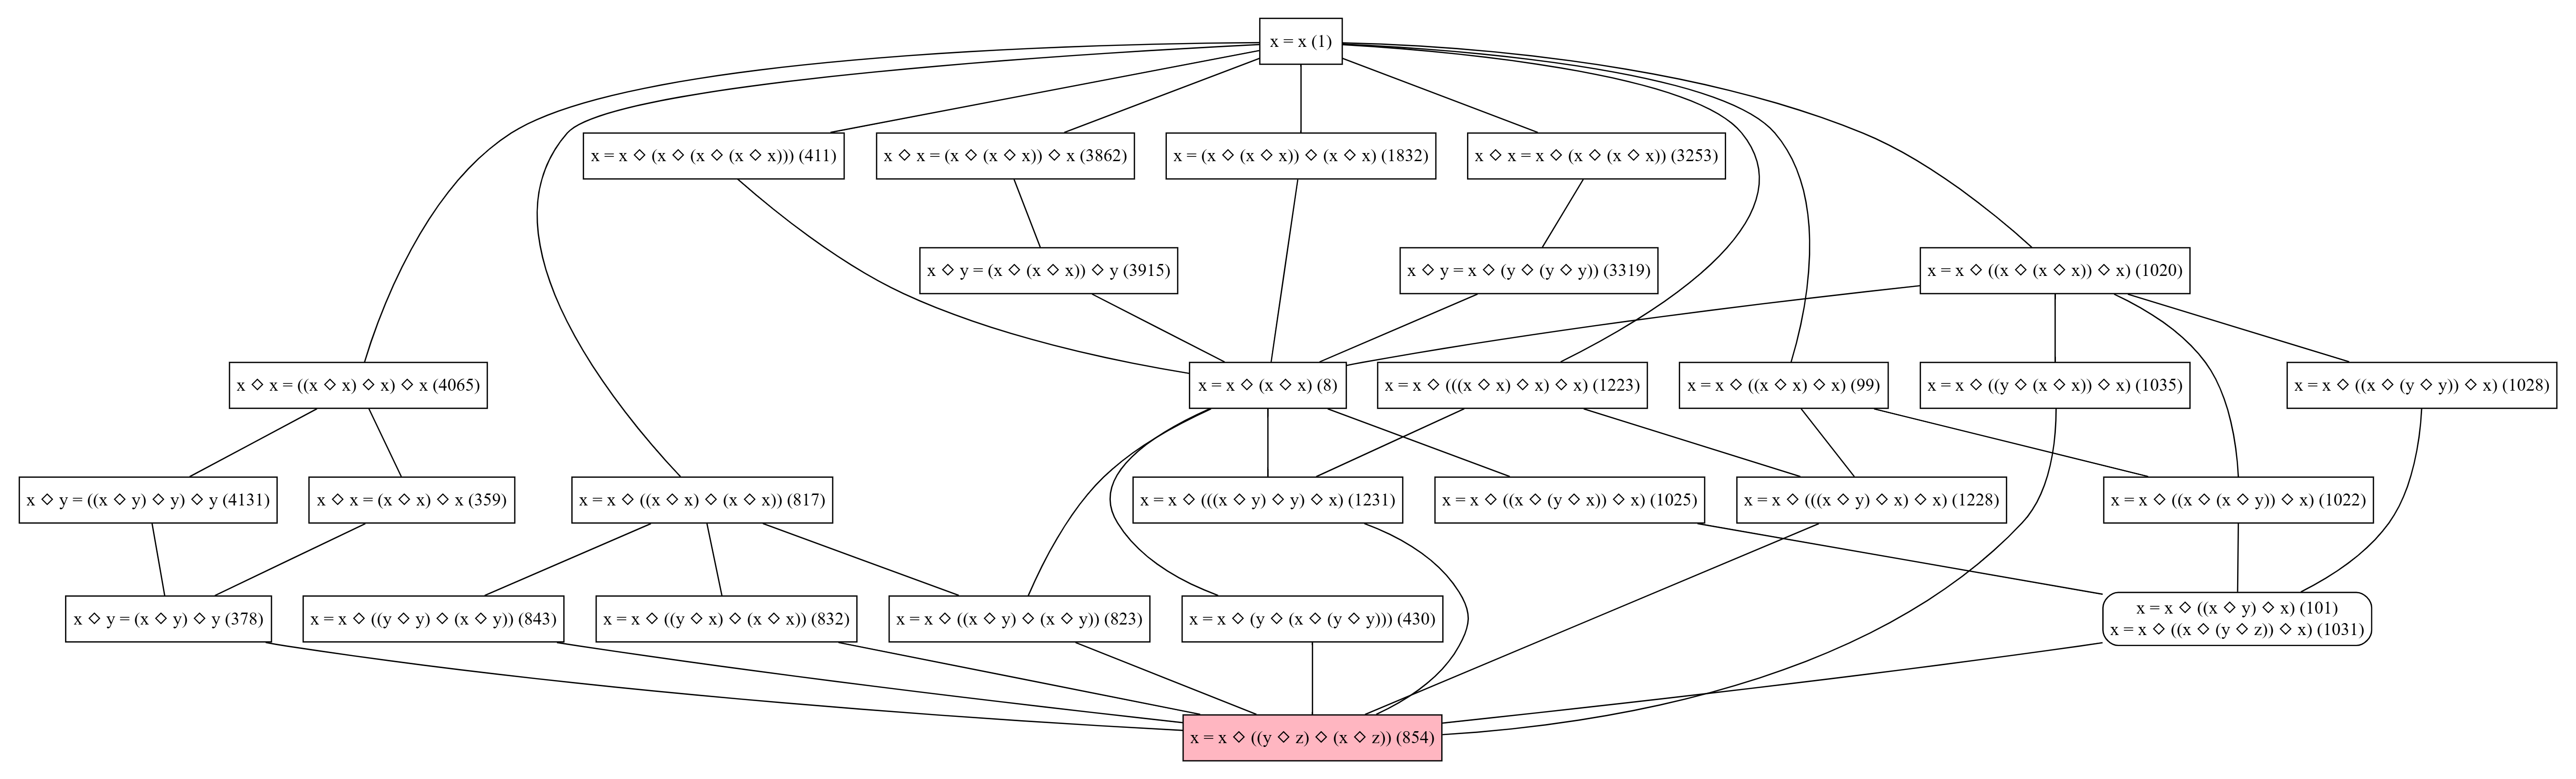
\includegraphics[width=0.85\textwidth]{854.png}
\caption{A Hasse diagram of all the equational laws implied by \Cref{eq854}.  An edge in this diagram indicates that the lower equation implies the higher one. Rounded rectangles indicate groups of equivalent laws.  This graph was produced by the visualization tool \emph{Graphiti}, which was developed for this project.}
\label{fig:854}
\end{figure}


Of the $22033636$ possible implications $E \vdash E'$, $8178279$ (or $37.12\%$) would end up being true. To establish such positive implications $E \vdash E'$, the main techniques used were as follows:

\begin{itemize}
    \item A very small number of positive implications were established and formalized by hand, mostly through direct rewriting of the laws; but this approach would not scale to the full project.
    \item Simple rewriting rules, for instance based on the observation that any law of the form $\x \formaleq f(\y,\z,\dots)$ was necessarily equivalent to the trivial law \Cref{eq2}, could already reduce the size of potential equivalence classes by a significant fraction. We discuss this method in \Cref{rewrite-sec}.
    \item The preorder axioms for $\vdash$, as well as the ``duality'' symmetry of the preorder with respect to replacing a magma operation $x \op y$ with its opposite $x \op^{\mathrm{op}} y \coloneqq y \op x$, can be used to significantly cut down on the number of implications that need to be proven explicitly; ultimately, only $10657$ ($0.05\%$) of the positive implications needed a direct proof.
    \item Automated Theorem Provers (ATP) could be deployed at extremely fast speeds to establish a complete generating set of positive implications; see \Cref{automated-sec}.
\end{itemize}

More challenging were the $13855357$ ($62.88\%$) implications that were false, $E \not \vdash E'$. Here, the range of techniques needed to refute such implications were quite varied.
\begin{itemize}
        \item Syntactic methods, such as observing an ``matching invariant'' of the law $E$ that was not shared by the law $E'$, could be used to obtain some refutations.  For instance, if both sides of $E$ had the same order, but both sides of $E'$ did not, this could be used to syntactically refute $E \vdash E'$.  Similarly, if the law $E$ was confluent, enjoyed a complete rewriting system, or otherwise permitted some understanding of the free magma associated to that law, one could decide the assertions $E \vdash E'$ for all possible laws $E'$, or at least a significant fraction of such laws.  We discuss these methods, and the extent to which they can be automated in \Cref{syntactic-sec}.
        \item Small finite magmas, which can be described explicitly by multiplication tables, could be tested by brute force computations to provide a large number of counterexamples to implications, or by ATP-assisted methods. See \Cref{finite-sec}.
        \item Linear models, in which the magma operation took the form $x \op y = ax + by$ for some (commuting or non-commuting) coefficients $a,b$, allowed for another large class of counterexamples to implications, which could be automatically scanned for either by brute force or by Grobner basis type calculations. See \Cref{linear-sec}.
        \item Translation invariant models, in which the magma operation took the form $x \op y = x + f(y-x)$ on an additive group, or $x \op y = x f(x^{-1} y)$ on a non-commutative group, reduce matters to analyzing certain functional equations; see \Cref{translation-sec}.
        \item Greedy methods, in which either the multiplication table $(x,y) \mapsto x \op y$ or the function $f$ determining a translation-invariant model are iteratively constructed by a greedy algorithm subject to a well-chosen ruleset, were effective in resolving many implications not easily disposed of by preceding methods. See \Cref{greedy-sec}.
        \item Starting with a simple base magma $M$ obeying both $E$ and $E'$, and either enlarging it to a larger magma $M' \supset M$, extending it to a magma $N$ with a projection homomorphism $\pi: N \to M$, or modifying the multiplication table on a small number of values, also proved effective when combined with greedy methods. See \Cref{modify-base}.
        \item To each equation $E$ one can associate a ``twisting semigroup'' $S_E$.  If $S_E$ is larger than $S_{E'}$, then this can often be used to disprove the implication $E \vdash E'$; see \Cref{twisting-sec}.
        \item Some \emph{ad hoc} models based on existing mathematical objects, such as infinite trees, rings of polynomials, or ``Kisielewicz models'' utilizing the prime factorization of the natural numbers, could also handle some otherwise difficult cases.  In some cases, the magma law induced some relevant and familiar structures, such as a directed graph or a partial order, which also helped guide counterexample constructions. See \Cref{adhoc-sec}.
        \item Automated theorem provers were helpful in identifying which simplifying axioms could be added to the magma without jeopardizing the ability to refute the desired implication $E \vdash E'$.
\end{itemize}

\subsection{Extensions}

While the primary objective of the ETP was being completed, some additional related results were generated as spinoffs.  Specifically:
\begin{itemize}
\item In \Cref{finite-sec} we report on a variant of the implication graph of the original set of 4692 equations, in which the magma is required to be finite.
\item In \Cref{order-5} we report on classifying which of the $57882$ distinct laws of order $5$ are equivalent to the singleton law \Cref{eq2}, either with or without the requirement that the magma be finite.
\item In \Cref{higman-neumann} we report on classifying the laws of order $8$ that are equivalent to the Higman-Neumann law \Cref{eq42323216}.
\end{itemize}

\note{Also mention ML stuff, GUI}

\chapter{Selected laws}\label{subgraph-eq}

In this project we study the 4694 laws (up to symmetry and relabeling) of total order at most $4$.

Selected laws of interest are listed below, as well as in \href{https://github.com/teorth/equational_theories/blob/main/equational_theories/Equations/Basic.lean}{this file}.

\begin{definition}[Equation 1]\label{eq1}\lean{Equation1}\leanok\uses{magma-def}  Equation 1 is the law $0 \formaleq 0$ (or the equation $x=x$).
\end{definition}

This is the trivial law, satisfied by all magmas. It is self-dual.


\begin{definition}[Equation 2]\label{eq2}\lean{Equation2}\leanok\uses{magma-def}  Equation 2 is the law $0 \formaleq 1$ (or the equation $x=y$).
\end{definition}

This is the singleton law, satisfied only by the empty and singleton magmas.  It is self-dual.

\begin{definition}[Equation 3]\label{eq3}\lean{Equation3}\leanok\uses{magma-def}  Equation 3 is the law $0 \formaleq 0 \op 0$ (or the equation $x = x \op x$).
\end{definition}

This is the idempotence law.  It is self-dual.

\begin{definition}[Equation 4]\label{eq4}\lean{Equation4}\leanok\uses{magma-def}  Equation 4 is the law $0 \formaleq 0 \op 1$ (or the equation $x = x \op y$).
\end{definition}

This is the left absorption law.

\begin{definition}[Equation 5]\label{eq5}\lean{Equation5}\leanok\uses{magma-def}  Equation 5 is the law $0 \formaleq 1 \op 0$ (or the equation $x = y \op x$).
\end{definition}

This is the right absorption law (the dual of \Cref{eq4}).

\begin{definition}[Equation 6]\label{eq6}\lean{Equation6}\leanok\uses{magma-def}  Equation 6 is the law $0 \formaleq 1 \op 1$ (or the equation $x = y \op y$).
\end{definition}

This law is equivalent to the singleton law.

\begin{definition}[Equation 7]\label{eq7}\lean{Equation7}\leanok\uses{magma-def}  Equation 7 is the law $0 \formaleq 1 \op 2$ (or the equation $x = y \op z$).
\end{definition}

This law is equivalent to the singleton law.

\begin{definition}[Equation 8]\label{eq8}\lean{Equation8}\leanok\uses{magma-def}  Equation 8 is the law $0 \formaleq 0 \op (0 \op 0)$ (or the equation $x = x \op (x \op x)$).
\end{definition}

\begin{definition}[Equation 14]\label{eq14}\lean{Equation14}\leanok\uses{magma-def}  Equation 14 is the law $0 \formaleq  1 \op (0 \op 1)$ (or the equation $x = y \op (x \op y))$.
\end{definition}

Appears in Problem A1 from Putnam 2001.  See \Cref{29_equiv_14}.

\begin{definition}[Equation 16]\label{eq16}\lean{Equation16}\leanok\uses{magma-def}  Equation 16 is the law $0 \formaleq  1 \op (1 \op 0)$ (or the equation $x = y \op (y \op x))$.
\end{definition}

\begin{definition}[Equation 23]\label{eq23}\lean{Equation23}\leanok\uses{magma-def}  Equation 23 is the law $0 \formaleq  (0 \op 0) \op 0$ (or the equation $x = (x \op x) \op x$).
\end{definition}

This is the dual of \Cref{eq8}.

\begin{definition}[Equation 29]\label{eq29}\lean{Equation29}\leanok\uses{magma-def}  Equation 29 is the law $0 \formaleq  (1 \op 0) \op 1$ (or the equation $x = (y \op x) \op y)$.
\end{definition}

Appears in Problem A1 from Putnam 2001.  Dual to \Cref{eq14}.  See \Cref{29_equiv_14}.

\begin{definition}[Equation 38]\label{eq38}\lean{Equation38}\leanok\uses{magma-def}  Equation 38 is the law $0 \op 0  \formaleq  0 \op 1$ (or the equation $x \op x = x \op y$).
\end{definition}

This law asserts that the magma operation is independent of the second argument.

\begin{definition}[Equation 39]\label{eq39}\lean{Equation39}\leanok\uses{magma-def}  Equation 39 is the law $0 \op 0  \formaleq  1 \op 0$ (or the equation $x \op x = y \op x$).
\end{definition}

This law asserts that the magma operation is independent of the first argument (the dual of \Cref{eq38}).

\begin{definition}[Equation 40]\label{eq40}\lean{Equation40}\leanok\uses{magma-def}  Equation 40 is the law $0 \op 0  \formaleq  1 \op 1$ (or the equation $x \op x = y \op y$).
\end{definition}

This law asserts that all squares are constant. It is self-dual.

\begin{definition}[Equation 41]\label{eq41}\lean{Equation41}\leanok\uses{magma-def}  Equation 41 is the law $0 \op 0  \formaleq  1 \op 2$ (or the equation $x \op x = y \op z$).
\end{definition}

This law is equivalent to the constant law, \Cref{eq46}.

\begin{definition}[Equation 42]\label{eq42}\lean{Equation42}\leanok\uses{magma-def}  Equation 42 is the law $0 \op 1  \formaleq  0 \op 2$ (or the equation $x \op y = x \op z$).
\end{definition}

Equivalent to \Cref{eq38}.

\begin{definition}[Equation 43]\label{eq43}\lean{Equation43}\leanok\uses{magma-def}  Equation 43 is the law $0 \op 1  \formaleq  1 \op 0$ (or the equation $x \op y = y \op x$).
\end{definition}

The commutative law. It is self-dual.

\begin{definition}[Equation 45]\label{eq45}\lean{Equation45}\leanok\uses{magma-def}  Equation 45 is the law $0 \op 1  \formaleq  2 \op 1$ (or the equation $x \op y = z \op y$).
\end{definition}

This is the dual of \Cref{eq42}.

\begin{definition}[Equation 46]\label{eq46}\lean{Equation46}\leanok\uses{magma-def}  Equation 46 is the law $0 \op 1  \formaleq  2 \op 3$ (or the equation $x \op y = z \op w$).
\end{definition}

The constant law: all products are constant. It is self-dual.

\begin{definition}[Equation 63]\label{eq63}\lean{Equation63}\leanok\uses{magma-def}  Equation 63 is the law $0 \formaleq 1 \op (0 \op (0 \op 1))$ (or the equation $x = y \op (x \op (x \op y))$).
\end{definition}

The ``Dupont'' law, studied further in Section~\ref{dupont-section}.

\begin{definition}[Equation 65]\label{eq65}\lean{Equation65}\leanok\uses{magma-def}  Equation 65 is the law $0 \formaleq 1 \op (0 \op (1 \op 0))$ (or the equation $x = y \op (x \op (y \op x))$).
\end{definition}

The ``Asterix'' law, studied further in Section~\ref{asterix-section}.

\begin{definition}[Equation 168]\label{eq168}\lean{Equation168}\leanok\uses{magma-def}  Equation 168 is the law $0  \formaleq  (1 \op 0) \op (0 \op 2)$ (or the equation $x = (y \op x) \op (x \op z)$).
\end{definition}

The law of a central groupoid. It is self-dual.

\begin{definition}[Equation 206]\label{eq206}\lean{Equation206}\leanok\uses{magma-def}  Equation 206 is the law $0  \formaleq  (0 \op (0 \op 1)) \op 1$ (or the equation $x = (x \op (x \op y)) \op y$).
\end{definition}

Our project located this law as one member of an ``Austin pair''; see Chapter \ref{infinite-model-chapter}. The infinite counterexample is constructed using the infinite 3-regular tree.

\begin{definition}[Equation 381]\label{eq381}\lean{Equation381}\leanok\uses{magma-def}  Equation 381 is the law $0 \op 1  \formaleq  (0 \op 2) \op 1$ (or the equation $x \op y = (x \op z) \op y$).
\end{definition}

Appears in Putnam 1978, Problem A4, part (b).

\begin{definition}[Equation 387]\label{eq387}\lean{Equation387}\leanok\uses{magma-def}  Equation 387 is the law $0 \op 1  \formaleq  (1 \op 1) \op 0$ (or the equation $x \op y = (y \op y) \op x$).
\end{definition}

Introduced in \href{https://mathoverflow.net/a/450905/766}{MathOverflow}. See \Cref{387_implies_43}

\begin{definition}[Equation 477]\label{eq477}\lean{Equation477}\leanok\uses{magma-def}  Equation 477 is the law $0 \formaleq 1 \op (0 \op (1 \op (1 \op 1)))$ (or the equation $x = y \op (x \op (y \op (y \op y)))$).
\end{definition}

An example of a confluent law; see \Cref{477-confl}.

\begin{definition}[Equation 854]\label{eq854}\lean{Equation953}\leanok\uses{magma-def}  Equation 854 is the law $0 = 0 \op ((1 \op 2) \op (0 \op 2))$ (or the equation $x = x \op ((y \op z) \op (x \op z))$).
\end{definition}

Studied in \Cref{854-chapter}


\begin{definition}[Equation 953]\label{eq953}\lean{Equation953}\leanok\uses{magma-def}  Equation 953 is the law $0 = 1 \op ((2 \op 0) \op (2 \op 2))$ (or the equation $x = y \op ((z \op x) \op (z \op z))$).
\end{definition}

An example of a trivial law; see \Cref{953_equiv_2}.

\begin{definition}[Equation 1485]\label{eq1485}\lean{Equation1491}\leanok\uses{magma-def}  Equation 1485 is the law $0 \formaleq  (1 \op 0) \op (0 \op (2 \op 1))$ (or the equation $x = (y \op x) \op (x \op (z \op y))$).
\end{definition}

The ``Obelix'' law, studied further in Section~\ref{asterix-section}.

\begin{definition}[Equation 1491]\label{eq1491}\lean{Equation1491}\leanok\uses{magma-def}  Equation 1491 is the law $0 \formaleq  (1 \op 0) \op (1 \op (1 \op 0))$ (or the equation $x = (y \op x) \op (y \op (y \op x))$).
\end{definition}

The ``Obelix'' law, studied further in Section~\ref{asterix-section}.

\begin{definition}[Equation 1571]\label{eq1571}\lean{Equation1571}\leanok\uses{magma-def}  Equation 1571 is the law $0 \formaleq  (1 \op 2) \op (1 \op (0 \op 2))$ (or the equation $x = (y \op z) \op (y \op (x \op z))$).
\end{definition}

Introduced in \cite{mendelsohn-padmanabhan}.  As shown in \Cref{1571_impl}, this law characterizes abelian groups of exponent two.

\begin{definition}[Equation 1648]\label{eq1648}\lean{Equation1648}\leanok\uses{magma-def}  Equation 1648 is the law $0 \formaleq  (0 \op 1) \op ((0 \op 1) \op 1)$ (or the equation $x = (x \op y) \op ((x \op y) \op y)$).
\end{definition}

The golden ratio is a coefficient of the linearization of this law.

\begin{definition}[Equation 1657]\label{eq1657}\lean{Equation1657}\leanok\uses{magma-def}  Equation 1657 is the law $0 \formaleq  (0 \op 1) \op ((1 \op 1) \op 0)$ (or the equation $x = (x \op y) \op ((y \op y) \op x)$).
\end{definition}

\begin{definition}[Equation 1659]\label{eq1659}\lean{Equation1659}\leanok\uses{magma-def}  Equation 1659 is the law $0 \formaleq  (0 \op 1) \op ((1 \op 1) \op 2)$ (or the equation $x = (x \op y) \op ((y \op y) \op z)$).
\end{definition}

\begin{definition}[Equation 1661]\label{eq1661}\lean{Equation1661}\leanok\uses{magma-def}  Equation 1661 is the law $0 \formaleq  (0 \op 1) \op ((1 \op 2) \op 1)$ (or the equation $x = (x \op y) \op ((y \op z) \op y)$).
\end{definition}

These two laws admit infinite models on the natural numbers arising from the modified base model construction. See Section~\ref{infinite-examples-section}.

\begin{definition}[Equation 1689]\label{eq1689}\lean{Equation1689}\leanok\uses{magma-def}  Equation 1689 is the law $0 \formaleq  (1 \op 0) \op ((0 \op 2) \op 2)$ (or the equation $x = (y \op x) \op ((x \op z) \op z)$).
\end{definition}

Mentioned in \cite{Kisielewicz2}.  See \Cref{1689_equiv_2}.

\begin{definition}[Equation 1701]\label{eq1701}\lean{Equation1701}\leanok\uses{magma-def}  Equation 1701 is the law $0 \formaleq  (1 \op x) \op ((2 \op 0) \op 0)$ (or the equation $x = (y \op x) \op ((z \op x) \op x)$).
\end{definition}

This law admits infinite models on the natural numbers arising from the modified base model construction. See Section~\ref{infinite-examples-section}.

\begin{definition}[Equation 2662]\label{eq2662}\lean{Equation2662}\leanok\uses{magma-def}  Equation 2662 is the law $0 \formaleq  ((0 \op 1) \op (0 \op 1)) \op 0$ (or the equation $x = ((x \op y) \op (x \op y)) \op x$).
\end{definition}

Appears in \cite{mendelsohn-padmanabhan}.

\begin{definition}[Equation 3167]\label{eq3167}\lean{Equation3167}\leanok\uses{magma-def}  Equation 3167 is the law $0 \formaleq  (((1 \op 1) \op 2) \op 2) \op 0$ (or the equation $x = (((y \op y) \op z) \op z) \op x$).
\end{definition}


\begin{definition}[Equation 3588]
  \label{eq3588}\lean{Equation3588}\leanok\uses{magma-def}
  Equation 3588 is the law $0 \op 1 \formaleq 2 \op ((0 \op 1) \op 2)$ (or the equation $x \op y = z \op ((x \op y) \op z)$).
\end{definition}

Our project located this law as one member of an ``Austin pair''; see Chapter \ref{infinite-model-chapter}.

\begin{definition}[Equation 3722]\label{eq3722}\lean{Equation3722}\leanok\uses{magma-def}  Equation 3722 is the law $0 \op 1  \formaleq  (0 \op 1) \op (0 \op 1)$ (or the equation $x \op y = (x \op y) \op (x \op y)$).
\end{definition}

Appears in Putnam 1978, Problem A4, part (a).  It is self-dual.

\begin{definition}[Equation 3744]\label{eq3744}\lean{Equation3744}\leanok\uses{magma-def}  Equation 3744 is the law $0 \op 1  \formaleq  (0 \op 2) \op (3 \op 1)$ (or the equation $x \op y = (x \op z) \op (w \op y)$).
\end{definition}

This law is called a ``bypass operation'' in Putnam 1978, Problem A4. It is self-dual.  See \Cref{3744_implies_3722_381}.

\begin{definition}[Equation 3994]
  \label{eq3994}\uses{magma-def}
  Equation 3994 is the law $0 \op 1 \formaleq (2 \op (0 \op 1)) \op 2$ (or the equation $x \op y = (z \op (x \op y)) \op z$).
\end{definition}

Our project located this law as one member of an ``Austin pair''; see Chapter \ref{infinite-model-chapter}.

\begin{definition}[Equation 4315]\label{eq4315}\lean{Equation4315}\leanok\uses{magma-def}  Equation 4315 is the law $0 \op (1 \op 0)  \formaleq  0 \op (1 \op 2)$ (or the equation $x \op (y \op x) = x \op (y \op z)$).
\end{definition}

\begin{definition}[Equation 4512]\label{eq4512}\lean{Equation4512}\leanok\uses{magma-def}  Equation 4512 is the law $0 \op (1 \op 2)  \formaleq  (0 \op 1) \op 2$ (or the equation $x \op (y \op z) = (x \op y) \op z$).
\end{definition}

The associative law. It is self-dual.

\begin{definition}[Equation 4513]\label{eq4513}\lean{Equation4513}\leanok\uses{magma-def}  Equation 4513 is the law $0 \op (1 \op 2)  \formaleq  (0 \op 1) \op 3$ (or the equation $x \op (y \op z) = (x \op y) \op w$).
\end{definition}

\begin{definition}[Equation 4522]\label{eq4522}\lean{Equation4522}\leanok\uses{magma-def}  Equation 4522 is the law $0 \op (1 \op 2)  \formaleq  (0 \op 3) \op 4$ (or the equation $x \op (y \op z) = (x \op w) \op u$).
\end{definition}

Dual to \Cref{eq4579}.

\begin{definition}[Equation 4564]\label{eq4564}\lean{Equation4564}\leanok\uses{magma-def}  Equation 4564 is the law $0 \op (1 \op 2)  \formaleq  (3 \op 1) \op 2$ (or the equation $x \op (y \op z) = (w \op y) \op z$).
\end{definition}

Dual to \Cref{eq4513}.

\begin{definition}[Equation 4579]\label{eq4579}\lean{Equation4579}\leanok\uses{magma-def}  Equation 4579 is the law $0 \op (1 \op 2)  \formaleq  (3 \op 4) \op 2$ (or the equation $x \op (y \op z) = (w \op u) \op z$).
\end{definition}

Dual to \Cref{eq4522}.

\begin{definition}[Equation 4582]\label{eq4582}\lean{Equation4582}\leanok\uses{magma-def}  Equation 4582 is the law $0 \op (1 \op 2)  \formaleq  (3 \op 4) \op 5$ (or the equation $x \op (y \op z) = (w \op u) \op v$).
\end{definition}

This law asserts that all triple constants (regardless of bracketing) are constant.

\section{Equations of order greater than \texorpdfstring{$4$}{4}}

We note some selected laws of order more than $5$, which are used in some later chapters of the blueprint.

\begin{definition}[Equation 5093]
  \label{eq5093}\uses{magma-def}\lean{Equation5093}\leanok
  Equation 5093 is the law $0  \formaleq 1 \op (1 \op (1 \op (0 \op (2 \op 1))))$ (or the equation $x = y \op (y \op (y \op (x \op (z \op y))))$).
\end{definition}

This law of order $5$ was mentioned in \cite{Kisielewicz2}.  See \Cref{5093-nontrivial}.

\begin{definition}[Equation 26302]
  \label{eq26302}\uses{magma-def}
  Equation 26302 is the law $0  \formaleq (1 \op ((2 \op 0) \op 3)) \op (0 \op 3)$ (or the equation $x = (y \op ((z \op x) \op w)) \op (x \op w)$).
\end{definition}

A law that characterizes natural central groupoids; see \Cref{natural-central-groupoid}.

\begin{definition}[Equation 28770]
  \label{eq28770}\uses{magma-def}\lean{Equation28770}\leanok
  Equation 28770 is the law $0  \formaleq  (((1 \op 1) \op 1) \op 0) \op (1 \op 2)$ (or the equation $x = (((y \op y) \op y) \op x) \op (y \op z)$).
\end{definition}

This law of order $5$ was introduced by Kisielewicz \cite{Kisielewicz}. See \Cref{kis-thm2}.

\begin{definition}[Equation 345169]
  \label{eq345169}\uses{magma-def}
  Equation 345169 is the law $0  \formaleq  (1 \op ((0 \op 1) \op 1)) \op (0 \op (2 \op 1))$ (or the equation $x = (y \op ((x \op y) \op y)) \op (x \op (z \op y))$).
\end{definition}

This law of order $6$ was shown in \cite{mccune_et_al} to characterize the Sheffer stroke in a boolean algebra; see \Cref{sheffer}.

\begin{definition}[Equation 374794]
  \lean{Equation374794}\leanok
  \label{eq374794}\uses{magma-def}
  Equation 374794 is the law $0  \formaleq  (((1 \op 1) \op 1) \op 0) \op ((1 \op 1) \op 2)$ (or the equation $x = (((y \op y) \op y) \op x) \op ((y \op y) \op z)$).
\end{definition}

This law of order $6$ was introduced by Kisielewicz \cite{Kisielewicz}; see \Cref{kis-thm}.

\chapter{Infinite models}\label{infinite-model-chapter}

In this chapter we consider non-implications which are refuted only on infinite models, as those are
more challenging to prove---they can't be proved by directly giving an operation table and checking
which laws it satisfies.

The singleton or empty magma obeys all equational laws.  One can ask whether an equational law admits nontrivial finite or infinite models.  An \emph{Austin law} is a law which admits infinite models, but no nontrivial finite models.  Austin \cite{austin} established the first such law, namely the order $9$ law
$$ (((1 \op 1) \op 1) \op 0) \op (((1 \op 1) \op ((1 \op 1) \op 1)) \op 2) \formaleq 0.$$
A shorter Austin law of order $6$ was established in \cite{Kisielewicz}:

\begin{theorem}[Kisielewicz's first Austin law]
  \lean{InfModel.Finite.Equation374794_implies_Equation2,InfModel.Equation374794_not_implies_Equation2}\leanok
  \label{kis-thm}\uses{eq374794,eq2}
  \Cref{eq374794} is an Austin law.
\end{theorem}

\begin{proof} \leanok  First we show that every finite model of \Cref{eq374794} is trivial.  Write $y^2 := y \op y$ and $y^3 := y^2 \op y$.  For any $y,z$, introduce the functions ${f_y: x \mapsto y^3 \op x}$ and ${g_{yz}: x \mapsto x \op (y^2 \op z)}$.  \Cref{eq374794} says that $g_{yz}(f_y(x))=x$, hence by finiteness $g_{yz}=f_y^{-1}$, showing that $g_{yz}$ does not depend on the value of $z$.  Since
$$ f_y(y^2 \op z) = g_{yz}(y^3),$$
it follows that $f_y(y^2 \op z)=f_y(y^3)$ which by injectivity of $f_y$ implies that $z\mapsto y^2 \op z$ is a constant function (with $y$ fixed).  Substituting $y^2$ for $y$ shows that the same is true for $z\mapsto (y^2 \op y^2) \op z$, and since
$$ f_y(z) = (y^2 \op y) \op z = (y^2 \op y^2) \op z$$
we conclude that $f_y$ is also a constant function.  But this function is already known to be injective, thus there do not exist distinct elements in its domain, showing that the model must be trivial.

To construct an infinite model, consider the magma of positive integers $\Z^+$ with the operation $x \op y$ defined by
$$
x \op y =
\begin{cases}
2^y, & x=  y            \\
3^y, & x=  1,\ y \neq 1 \\
  z, & x=3^z,\ y \neq x \\
  1, & else
\end{cases}.
$$
Then $y \op y = 2^y$ and $(y \op y) \op y = 1$ for all $y$.  If $x\neq 1$ we have that
$$ ((y \op y) \op y) \op x = 3^x, $$
and since $(y \op y) \op z$ is a power of two for all $y, z$ it follows that
$$ 3^x \op ((y \op y) \op z) = x. $$
The case $x=1$ requires a further argument: observe that $w = (y \op y) \op z$ evaluates to one unless $z = 2^y$, in which case it evaluates to $2^{2^y}$ (which is greater than or equal to four).  In particular, $w$ never takes the value two.  Thus
$$ (((y \op y) \op y) \op 1) \op ((y \op y) \op z) = 2 \op w = 1, $$
concluding our proof that this magma is a model of \Cref{eq374794}
\end{proof}

An even shorter law (order $5$) was obtained by the same author in a follow-up paper \cite{Kisielewicz2}:

\begin{theorem}[Kisielewicz's second Austin law]\label{kis-thm2}\uses{eq2, eq28770}\lean{InfModel.Finite.Equation28770_implies_Equation2}\lean{InfModel.Equation28770_not_implies_Equation2}\leanok \Cref{eq28770} is an Austin law.
\end{theorem}

\begin{proof} \leanok Using the $y^2$ and $y^3$ notation as before, the law reads
\begin{equation}\label{kis2-law}
   x = (y^3 \op x) \op (y \op z).
  \end{equation}
In particular, for any $y$, the map $T_y \colon x \mapsto y^3 \op x$ is injective, hence bijective in a finite model $G$.  In particular we can find a function $f : G \to G$ such that $T_y f(y) = y^3$ for all $y$  Applying \Cref{kis2-law} with $x = f(y)$, we conclude
$$ T_y(y \op z) = y^3 \op (y \op z) = f(y) $$
and thus $y \op z$ is independent of $z$ by injectivity of $T_y$.  Thus, the left-hand side of \Cref{kis2-law} does not depend on $x$, and so the model is trivial.  This shows there are no non-trivial finite models.

To establish an infinite model, use $\N$ with $x \op y$ defined by requiring
$$ y \op y = 2^y; \quad 2^y \op y = 3^y$$
and
$$ 3^y \op x = 3^y 5^x$$
for $x \neq 3^y$, and
$$ (3^y 5^x) \op z = x$$
for $z \neq 3^y 5^x$.  Finally set
$$ 2^{3^y} \op z = 3^y$$
for $z \neq 3^y, 2^{3^y}$.  All other assignments of $\op$ may be made arbitrarily. It is then a routine matter to establish \Cref{kis2-law}.
\end{proof}

In that paper a computer search was also used to show that no law of order four or less is an Austin law.

An open question is whether \Cref{eq5093} is an Austin law.  We have the following partial result from \cite{Kisielewicz2}:

\begin{theorem}[Equation 5093 has no non-trivial finite models]\lean{InfModel.Finite.Equation5093_implies_Equation2}\leanok\label{5093-nontrivial}\uses{eq5093, models-def} \Cref{eq5093} has no non-trivial finite models.
\end{theorem}

\begin{proof} \leanok From \Cref{eq5093} we see that the map $w \mapsto y \op w$ is onto, hence injective in a finite model.  Using this injectivity four times in \Cref{eq5093}, we see that $z \op y$ does not depend on $z$, hence the expression
$x \op (z \op y)$ does not depend on $x$.  By \Cref{eq5093} again, this means that $x$ does not depend on $x$, which is absurd in a non-trivial model.
\end{proof}

We also have such a non-implication involving two laws of order $4$:

\begin{theorem}[3994 implies 3588 for finite models]\label{finite_imp_3994_3588_thm}\uses{eq3994,eq3588,models-def}
  \lean{InfModel.Finite.Equation3994_implies_Equation3588}\leanok
  All finite magmas which satisfy \Cref{eq3994} also satisfy \Cref{eq3588}.
\end{theorem}

\begin{proof}\label{finite_imp_3994_3588} \leanok
  For a finite magma $M$, consider the set $S = \{x \op y | x, y \in M\}$.
  Now $f_z : x \mapsto z \op x$ and $g_z : x \mapsto x \op z$.
  They both map $S$ to $S$, and due to the hypothesis $g_z \op f_z$ is the identity on $S$,
  so because $S$ is finite $f_z$ and $g_z$ must be inverse bijections on it, and therefore
  they commute.
\end{proof}

\begin{theorem}[3994 does not imply 3588 for infinite models]\label{non_imp_3994_3588_thm}\uses{eq3994,eq3588,models-def}
  \lean{InfModel.Equation3994_not_implies_Equation3588}\leanok
  There exists a magma which satisfies \Cref{eq3994} and not \Cref{eq3588}.
\end{theorem}

\begin{proof} \leanok
  Consider $\mathbb{N}$, with $x \op y$ defined as $x \oplus y$ (bitwise XOR) if $x$ and $y$ are even,
  $y+2$ if only $y$ is even, $x \dot - 2$ if only $x$ is even, and $0$ if both are odd.
  Note that the range of the operation is the set of even naturals.
  \Cref{eq3994} is satisfied, because for even $z$ we get $z \oplus (x \op y) \oplus z = x \op y$
  and for odd $z$ we get $(x \op y) + 2 \dot - 2 = x \op y$.
  Setting $x = y = z = 1$, \Cref{eq3588} isn't satisfied.
\end{proof}

The following result was established in \cite{austin_finite}:

\begin{theorem}[Austin's finite model theorem]\label{austin-two}\uses{models-def}\lean{InfModel.Finite.two_variable_laws}\leanok Any law with at most two variables has a non-trivial finite model.
\end{theorem}

\begin{proof} \leanok  If neither side of the law is a single variable then the zero law $x \op y = 0$ will work, so one can assume the law takes the form $x = f(x,y)$.  Consider a finite field $F$ with the operation $x \op y := ax+by$ for some coefficients $a,b \in F$.  Then the law becomes a pair of equations $P(a,b)=0$, $Q(a,b)=1$ in the coefficients for some polynomials $P,Q$ with integer coefficients, which one can verify to not divide each other (they have the same degree, and do not have the same set of non-zero monomials).  From Bezout's theorem, this equation has a solution in some field, and hence by the Lefschetz principle it has a solution in a finite field.
\end{proof}

Many implications for finite magmas rely on the fact that if $f, g:X \to X$ are functions on a finite set $X$, then $f \circ g = I$ if and only if $g \circ f = I$.  Two more complicated variants of this are as follows.

\begin{lemma}\label{ffg} \lean{FiniteModel.Finite.f_ffg_implies_f_fgf} \leanok Let $X$ be finite, and let $f, g: X \to X$ be such that $f = f \circ f \circ g$.  Then $f = f \circ g \circ f$.
\end{lemma}

\begin{proof} \leanok Call a point $x \in X$ \emph{periodic} if $f^n(x) = x$ for some $n>0$.  Because the forward orbit $x, f(x), f^2(x), \dots$ in a finite space $X$ must repeat, we see that for each $x$ there exists an $n$ such that $f^n(x)$ is periodic.  Let $n_x$ be the first $n$ for which this occurs.  If $n_x > 1$, then $g(x), f(g(x)), f(f(g(x))$ cannot be periodic (as this would imply $f(x)$ periodic), and then we can see that $n_{g(x)} = n_x + 1$.  Hence the maximal value of $n_x$ is at most $1$, which implies that $f(x)$ is periodic for every $x$.  Thus there is an $n > 1$ such that $f^n = f$.  Since $f = f^2 \circ g$, we have $f^n = f^{n-2} \circ f \circ f = f^{n-2} \circ (f^2 \circ g) \circ f = f^n \circ g \circ f = f \circ g \circ f$, as desired.
\end{proof}

\begin{lemma}\label{gff} \lean{FiniteModel.Finite.f_gff_implies_f_fgf} \leanok Let $X$ be finite, and let $f, g: X \to X$ be such that $f = g \circ f \circ f$.  Then $f = f \circ g \circ f$.
\end{lemma}

\begin{proof} \leanok By hypothesis, $f^2(x)$ uniquely determines $f(x)$.  This prevents $n_x = 2$ for any $x$ (because if $n>2$ is such that $f^{n+2}(x) = f^2(x)$, then $f^{n+1}(x) \neq f(x)$), and hence also prevents $n_x > 2$ for any $x$.   So again we have $f(x)$ periodic for all $x$, so $f^n = f$ for some $n>1$.  Then $f = f^n = f \circ (g \circ f^2) \circ f^{n-2} = f \circ g \circ f^n = f \circ g \circ f$ as required.
\end{proof}

This can be used to obtain a few positive finite magma implications, for instance by setting $f,g$ to be left and right multiplication operators.  Another useful lemma is

\begin{lemma}[Eventual period]\label{period} \lean{FiniteModel.Finite.fn_periodic} \leanok  Let $X$ be finite and $f: X \to X$.  Then there exists $n \geq 1$ such that $f^{2n} = f^n$.
\end{lemma}

\begin{proof} \leanok By the pigeonhole principle, there exists $n \geq 1$, $m \geq 0$ such that $f^{m+n} = f^m$, which implies on iteration that $f^{m+mn} = f^m$ and hence $f^{2mn} = f^{mn}$, giving the claim.
\end{proof}

As a sample application, we have

\begin{corollary}[3342]\label{3342} \lean{Eq3342.Finite.Equation3342_implies_Equation3522,Eq3342.Finite.Equation3342_implies_Equation4118} \leanok  On a finite magma $M$, equation 3342, $x \op y= y \op (x \op (x \op x))$, implies
  equation 3522, $x \op y = x \op ((y \op y) \op y)$, as well as equation 4118, $x \op y = ((x \op x) \op x) \op y$.
\end{corollary}

\begin{proof}\uses{period} \leanok Write $Sx := x \op$, $fx := x \op Sx$ and $Cx = Sx \op x$, then we have $x \op y= y \op fx$, and our task is to show $x \op y = Cx \op y$ and $x \op y = x \op Cy$ for finite magmas, giving the four open implications.

Note that $x \op y= y \op fx = fx \op fy$, hence $f$ is a homomorphism.  By \Cref{period}, there is $n \geq 1$ with $f^n = f^{2n}$.  From 3342 we have $Sx = S fx$ and $Cx = Sx \op x = f^n Sx \op f^n x = f^n Sx \op f^{2n} x = f^{2n-1} x \op f^n Sx = f^{n-1} x \op S x = f(f^{n-1} x) = f^n x$.  Then
$$ Cx \op y = f^n x \op y = f^{2n} x \op f^n y = f^n x \op f^n y = x \op y$$
and a similar argument gives $x \op Cy = x \op y$.
\end{proof}

\begin{proposition}[1167 implies 1096]\label{1167-1096}
  For finite magmas, Equation 1167,
  $$ x = y \op ((z \op (y \op y)) \op x)$$
implies Equation 1096,
$$ x = y \op ((x \op (z \op y)) \op x).$$
\end{proposition}

\begin{proof} We write 1167 as
  $$ L_y L_{z \op Sy} = I,$$
hence $L_y$ is invertible and $L_{z \op Sy} L_y = I$.  In particular $L_{z \op Sy} Sy = y$, hence squaring is injective, hence surjective.  So 1167 can be rewritten as $L_{S^{-1} y} L_{z \op y} = I$, hence $L_{z \op y}$ is independent of $z$.  In particular
$$ L_{x \op (z \op y)} = L_{S^{-2} z \op (z \op y)} = L_{L_{S^{-2} z} L_{S^{-1} z \op S S^{-2} z} y} = L_y$$
by 1167, hence the right-hand side of 1096 is independent of $z$.  Replacing $z$ with $y$, the claim now follows from 1167.
\end{proof}

\begin{proposition}[1113 implies 1167]\label{1113-1167}
  For finite magmas, Equation 1113,
$$ x = y \op ((y \op (z \op y)) \op x)$$
implies Equation 1167,
  $$ x = y \op ((z \op (y \op y)) \op x).$$
\end{proposition}

\begin{proof}
1113 asserts that $L_y L_{y \op (z \op y)} = I$, hence $L_y$ is invertible and $L_{y \op (z \op y)} = L_y^{-1}$ does not depend on $z$.  Setting $z = y \op Sy$ we see from 1113 that $y \op (z \op y) = y$ and hence we have left-involution: $L_y = L_y^{-1}$. Replacing $y$ with $L_z y$ in 1113 we now get $L_{L_z y} L_{L_z y \op y} = I$, which since $L_{L_z y}$ is its own inverse gives
\begin{equation}\label{intermediate}
  L_{L_z y \op y} = L_{L_z y}.
\end{equation}
In particular
$$ R_y^3 z = L_{L_z y \op y} y = L_{L_z y} y = R_y^2 z$$
hence as $L_{R_y^2 z}$ is its own inverse
$$ y =L_{R_y^2 z} L_{R_y^2 z} y = L_{R_y^2 z} R_y^3 z =
L_{R_y^2 z} R_y^3 z = S( R_y^2 z).$$
Thus squaring is surjective, hence invertible.

Next, by \eqref{intermediate} we have $L_{z \op Sy} = L_w$ where $w = R_{Sy}^2 z$.  By \eqref{intermediate} and the fact that $L_w$ is its own inverse, we have
$$ L_w^2 w = w = L_{z \op Sy} Sy =L_w Sy,$$
hence $Sw = L_w w = Sy$.  As $S$ is injective, we have $L_w = L_y$, and then $L_y L_{z \op Sy} = L_y^2 = I$, giving 1167.
\end{proof}

\begin{proposition}[1441 implies 4067, 1443 implies 3055]\label{1441-4067-1443-3055}
  For finite magmas, Equation 1441,
$$ x = (x \op y) \op (x \op (x \op x))$$
implies Equation 4067,
$$ x \op x = ((x \op x) \op y) \op x,$$
and equation 1443,
$$ x = (x \op y) \op (x \op (x \op z))$$
implies Equation 3055,
$$ x = (((x \op x) \op y) \op x) \op x.$$
\end{proposition}

\begin{proof}
  Write $\tilde C x = x \op Sx$, then 1441 asserts that $R_{\tilde Cx} R_y x = x$.  Setting $$y=Sx$$ we get $x = S\tilde Cx$, so by finiteness $\tilde C Sx = x$.  Replacing $x$ with $Sx$ in 1441 we conclude $R_x R_y Sx = Sx$ which is 4067.

  Clearly 1443 implies 1441, hence 4067 by the previous implication, so that 3055 simplifies to $x = Sx \op x$.  Meanwhile, 1443 also implies $x = S(x \op (x \op z))$.  On taking square roots and using $S \tilde C = x$, we obtain $x \op (x \op z) = \tilde Cx$.  Appying this with $z = Sx$ we conclude $L_x \tilde Cx = \tilde Cx$, hence on replacing $x$ with $Sx$ we get $L_{Sx} x = x$ as required.
\end{proof}

\begin{proposition}[1681 implies 3877, 1701 implies 1035]\label{1681-3877-1701-1035}
  For finite magmas, Equation 1681,
$$ x = (y \op x) \op ((x \op x) \op x)$$
implies Equation 3877,
$$ x \op x = (y \op (x \op x)) \op x,$$
and Equation 1701,
$$ x = (y \op x) \op ((z \op x) \op x)$$
implies Equation 1035,
$$ x = x \op ((y \op (x \op x)) \op x).$$
\end{proposition}

\begin{proof} This is very similar to the previous proof.
  Write $Cx = Sx \op x$, then 1681 asserts $R_{Cx} L_y x = x$.  Again setting $y=Sx$ yields $x=SCx$ hence $x = CSx$, and on replacing $x$ with $Sx$ in 1681 one obtains 3877.

For the second part, we simplify to $x = x \op Sx$, while 1701 gives $x = S((z \op x) \op x)$ hence $(z \op x) \op x = Cx$, so $R_x Cx = Cx$, so $R_{Sx} x = x$ as required.
\end{proof}

\chapter{General implications}

We will be interested in seeing which laws imply which other laws, in the sense that magmas obeying the former law automatically obey the latter.  We will also be interested in \emph{anti-implications} showing that one law does \emph{not} imply another, by producing examples of magmas that obey the former law but not the latter. Here is a formal definition.

\begin{definition}[Implication]\label{impl}\uses{models-def}  A law $E$ is said to \emph{imply} another law $E'$ if $\{E\} \models E'$, or equivalently:
  $$ G \models w  \formaleq  w' \implies G \models w''  \formaleq  w''' \hbox{ for all magmas } G$$
Two laws are said to be \emph{equivalent} if they imply each other.
\end{definition}

\begin{lemma}[Pre-order]\leanok\label{pre-order}\uses{impl}  If we define $E \leq E'$ if $E$ implies $E'$, then this is a pre-order on the set of laws, and equivalence is an equivalence relation.
\end{lemma}

Note that we view the stronger law as less than or equal to the weaker law.  This is because the class of magmas that obey the stronger law is a subset of the class of magmas that obey the weaker law.  It is also consistent with the conventions of Lean's Mathlib.

\begin{proof}\leanok Trivial.
\end{proof}

Implications between the laws from Chapter \ref{subgraph-eq} are depicted in Figure \ref{fig:implications}.

\begin{figure}
  \centering
  \includegraphics[width=0.5\linewidth]{../../images/implications.png}
  \caption{Implications between the above equations, displayed as a Hasse diagram.}
  \label{fig:implications}
\end{figure}


\begin{lemma}[Maximal element]\label{maximal}\uses{pre-order}  The law $0  \formaleq  0$ is the maximal element in this pre-order.
\end{lemma}

\begin{proof} Trivial.
\end{proof}

\begin{lemma}[Minimal element]\label{minimal}\uses{pre-order}  The law $0  \formaleq  1$ is the minimal element in this pre-order.
\end{lemma}

\begin{proof} Trivial.
\end{proof}

Every magma $G$ has a \emph{reversal} $G^{\mathrm{op}}$, formed by by replacing the magma operation $\circ$ with its opposite $\circ^{\mathrm{op}}:(x,y) \mapsto y \circ x$. There is a natural isomorphism between these magmas, which induces an involution $w \mapsto w^{\mathrm{op}}$ on words $w \in M_X$.  Every law $w  \formaleq  w'$ then has a \emph{dual} $w^{\mathrm{op}}  \formaleq  (w')^{\mathrm{op}}$.

For instance, the dual of the law $0 \circ 1 = 0 \circ 2$ is $1 \circ 0 = 2 \circ 0$, which after relabeling is $0 \circ 1 = 2 \circ 1$.  A list of equations and their duals can be found \href{https://github.com/teorth/equational_theories/blob/main/data/dual_equations.md}{here}.  Of the 4694 equations under consideration, 84 are self-dual, leaving 2305 pairs of dual equations.

The pre-ordering on laws has a duality symmetry:

\begin{lemma}[Duality of laws]\label{duality}\uses{pre-order}  If $w  \formaleq  w'$ implies $w''  \formaleq  w'''$, then $w^{\mathrm{op}}  \formaleq  (w')^{\mathrm{op}}$ implies $w''^{\mathrm{op}}  \formaleq  (w''')^{\mathrm{op}}$.
\end{lemma}

\begin{proof} This follows from the fact that a magma $G$ satisfies a law $w  \formaleq  w'$ if and only if $G^{\mathrm{op}}$ satisfies $w^{\mathrm{op}}  \formaleq  (w')^{\mathrm{op}}$.
\end{proof}

Some equational laws can be ``diagonalized'':

\begin{theorem}[Diagonalization]\label{diag}  An equational law of the form
  \begin{equation}\label{prediag} F(x_1,\dots,x_n) = G(y_1,\dots,y_m),
  \end{equation}
  where $x_1,\dots,x_n$ and $y_1,\dots,y_m$ are distinct elements of the alphabet, implies the diagonalized law
$$ F(x_1,\dots,x_n) = F(x'_1,\dots,x'_n).$$
where $x'_1,\dots,x'_n$ are distinct from $x_1,\dots,x_n$
In particular, if $G(y_1,\dots,y_m)$ can be viewed as a specialization of $F(x'_1,\dots,x'_n)$, then these two laws are equivalent.
\end{theorem}

\begin{proof}  From two applications of \eqref{prediag} one has
$$ F(x_1,\dots,x_n) = G(y_1,\dots,y_m)$$
and
$$ F(x'_1,\dots,x'_n) = G(y_1,\dots,y_m)$$
whence the claim.
\end{proof}

Thus for instance, Definition \ref{eq7} is equivalent to Definition \ref{eq2}.

\begin{theorem}[Laws implied by the constant law]\label{constant-impl}\uses{impl,eq46}  If $w, w'$ each have order at least one, then the law $w \formaleq w'$ is implied by the constant law (Definition \ref{eq46}).  If exactly one of $w, w'$ has order zero, and the law $w \formaleq w'$ is not implied by the constant law.
\end{theorem}

\begin{proof} Routine.
\end{proof}

\begin{theorem}[Criterion for implication]\label{variable-impl}\uses{impl}\lean{Law.MagmaLaw.SameCount.derive}\leanok  If $w \formaleq w'$ is such that every variable appears the same number of times in both $w$ and $w'$, and $w \formaleq w'$ implies another law $w'' \formaleq w'''$, then every variable appears the same number of times in both $w''$ and $w'''$.
\end{theorem}

\begin{proof} Consider the magma $\mathrm{MS}$ of multisets over an arbitrary set $A$ (which can be seen as finitely suported maps $A\rightarrow \N$), with the multiset addition law $+$.  By hypothesis, this magma obeys $w \formaleq w'$, and hence $w'' \formaleq w'''$, giving the claim by comparing the orders of the elements of $A$ appearing in $w''$ and $w'''$ in this magma.
\end{proof}

\chapter{Implications between selected laws}\label{implications-chapter}

We collect here some notable implications between the the selected laws in \Cref{subgraph-eq}.   By \Cref{sound-complete}, every implication can basically be established by a finite number of rewrites.  In most cases, the sequence of rewrites is quite straightforward, and the implication is very easy, but we record some less obvious examples.

\begin{theorem}[387 implies 43]\label{387_implies_43}\uses{eq387,eq43}\lean{Subgraph.Equation387_implies_Equation43}\leanok  \Cref{eq387} implies \Cref{eq43}.
\end{theorem}

\begin{proof}\leanok (From \href{https://mathoverflow.net/a/450905/766}{MathOverflow}).
  By \Cref{eq387}, one has the law
\begin{equation}\label{387-again}
  (x \op x) \op y = y \op x.
\end{equation}
Specializing to $y=x \op x$, we conclude
$$(x \op x) \op (x \op x) = (x \op x) \op x$$
and hence by another application of \Cref{eq387} we see that $x \op x$ is idempotent:
\begin{equation}\label{idem}
  (x \op x) \op (x \op x) = x \op x.
\end{equation}
Now, replacing $x$ by $x \op x$ in \Cref{387-again} and then using \Cref{idem} we see that
$$ (x \op x) \op y = y \op (x \op x)$$
so in particular $x \op x$ commutes with $y \op y$:
\begin{equation}\label{op-idem} (x \op x) \op (y \op y) = (y \op y) \op (x \op x).
\end{equation}
Also, from two applications of \Cref{387-again} one has
$$(x \op x) \op (y \op y) = (y \op y) \op x = x \op y.$$
Thus \Cref{op-idem} simplifies to $x \op y = y \op x$, which is \Cref{eq43}.
\end{proof}

\begin{theorem}[29 equivalent to 14]\label{29_equiv_14} \uses{eq29,eq14}\lean{Subgraph.Equation29_implies_Equation14}\leanok  \Cref{eq29} is equivalent to \Cref{eq14}.
\end{theorem}

This result was posed as Problem A1 from Putnam 2001.

\begin{proof}\leanok\uses{duality} By \Cref{duality} it suffices to show that \Cref{eq29} implies \Cref{eq14}.  From \Cref{eq29} one has
  $$ x = ((x \op y) \op x) \op (x \op y)$$
  and also
  $$ y = (x \op y) \op x$$
  giving $x = y \op (x \op y)$, which is \Cref{eq14}.
\end{proof}

\begin{theorem}[14 implies 29]\label{14_implies_29} \uses{eq29,eq14}\lean{Subgraph.Equation14_implies_Equation29}\leanok  \Cref{eq14} implies \Cref{eq29}.
\end{theorem}

This result was posed as Problem A1 from Putnam 2001.

\begin{proof}\leanok
\end{proof}

The following result was Problem A4 on Putnam 1978.

\begin{theorem}[3744 implies 3722, 381]\label{3744_implies_3722_381}\uses{eq3744, eq3722, eq381}\lean{Subgraph.Equation3744_implies_Equation3722, Subgraph.Equation3744_implies_Equation381}\leanok \Cref{eq3744} implies \Cref{eq3722} and \Cref{eq381}.
\end{theorem}

\begin{proof}\leanok By hypothesis, one has
$$x \op y = (x \op z) \op (w \op y)
  $$
for all $x,y,z,w$.  Various specializations of this give
\begin{align}
 x \op y &= (x \op z) \op (y \op y) \label{381-1} \\
 x \op z &= (x \op z) \op (x \op z) \label{381-2} \\
(x \op z) \op y &= ((x \op z) \op (x \op z)) \op (y \op y) \label{381-3}.
\end{align}
\Cref{381-2} gives \Cref{eq3722}, while \Cref{381-1}, \Cref{381-2}, \Cref{381-3} gives
$$ x \op y = (x\op z) \op y$$
which is \Cref{eq381}.
\end{proof}

\begin{theorem}[1689 is equivalent to 2]\label{1689_equiv_2}\uses{eq1689, eq2}\lean{Subgraph.Equation1689_implies_Equation2, Subgraph.Equation2_implies_Equation1689}\leanok \Cref{eq1689} is equivalent to \Cref{eq2}.
\end{theorem}


\begin{proof}\leanok  The implication of \Cref{eq1689} from \Cref{eq2} is trivial.  The converse is a surprisingly long chain of implications; see pages 326--327 of \cite{Kisielewicz2}.  The initial law
$$ x = (y \op x) \op ((x \op z) \op z)$$
is used to obtain, in turn,
$$ x \op ((((x \op y) \op y) \op z) \op z) = (x \op y) \op y,$$
$$(x \op (y \op z)) \op (z \op ((z \op w) \op w)) = y \op z,$$
$$x \op (y \op ((y \op z) \op z)) = (x \op y) \op y,$$
$$((x \op (y \op z)) \op z) \op z = y \op z,$$
$$(x \op (y \op (z \op w))) \op (z \op w) = y \op (z \op w),$$
$$(x \op (y \op z)) \op (y \op z) = x \op (y \op z),$$
$$((x \op y) \op ((y \op z) \op z)) \op ((y \op z) \op z) = y,$$
$$((x \op y) \op ((y \op z) \op z)) \op ((y \op z) \op z) = ((x \op ((x \op y) \op ((y \op z) \op z))) \op ((y \op z) \op z)) \op ((y \op z) \op z),$$
$$ x \op ((x \op y) \op y) = x,$$
$$ x \op (x \op (y \op z)) = x,$$
$$ (x \op y) \op y = x \op y,$$
$$ (x \op x) \op x = x,$$
$$ (x \op y) \op y = y,$$
$$ x \op y = y.$$
\end{proof}

The following result was established in \cite{mendelsohn-padmanabhan}.

\begin{theorem}[Consequences of 1571]\label{1571_impl}\uses{eq1571, eq2662, eq40, eq23, eq8, eq16, eq14, eq43, eq4512}\lean{Subgraph.Equation1571_implies_Equation2662, Subgraph.Equation1571_implies_Equation40, Subgraph.Equation1571_implies_Equation23,Subgraph.Equation1571_implies_Equation8, Subgraph.Equation1571_implies_Equation16, Subgraph.Equation1571_implies_Equation43, Subgraph.Equation1571_implies_Equation4512}\leanok  Magmas obeying \Cref{eq1571} also obey \Cref{eq2662}, \Cref{eq40}, \Cref{eq23}, \Cref{eq8}, \Cref{eq16}, \Cref{eq14}, \Cref{eq43}, and \Cref{eq4512}, and are in fact abelian groups of exponent two.  Conversely, all abelian groups of exponent two obey \Cref{eq1571}.
\end{theorem}

\begin{proof}\leanok  Suppose that a magma $G$ obeys \Cref{eq1571}, thus
\begin{equation}\label{1571-again}
 x = (y \op z) \op (y \op (x \op z)).
\end{equation}
$$ x = ((x \op y) \op (x \op y)) \op ((x \op y) \op (x \op (x \op y)))$$
and
$$ x = (x \op y) \op (x \op (x \op y))$$
whence
$$x = ((x \op y) \op (x \op y)) \op x$$
which is \Cref{eq2662}.  This gives
$$y = ((y \op z) \op (y \op z)) \op y$$
while from \Cref{1571-again} one has
$$ (y \op z) \op (y \op z) = (x \op y) \op (x \op ((y \op z) \op (y \op z) \op y))$$
whence
$$ (x \op y) \op (x \op y) = (y \op z) \op (y \op z).$$
This implies that $(x \op y) \op (x \op y)$ does not depend on $x$, or on $y$, hence is equal to some constant $e$:
$$ (x \op y) \op (x \op y) = e.$$
From \Cref{1571-again} the magma operation is surjective, hence
\begin{equation}\label{xxe} x \op x = e
\end{equation}
which gives \Cref{eq40}.  Applying \Cref{1571-again} with $x=y=z$ we conclude
$$ x = e \op (x \op e)$$
while if we instead take $y=z=e$ we have
$$ x = e \op (e \op (x \op e))$$
hence
$$ x = e \op x$$
and then also
$$ x = x \op e$$
from which we readily conclude \Cref{eq23}, \Cref{eq8}; thus $e$ is an identity element.  From \Cref{1571-again} with $z=e$ we now have
\begin{equation}\label{16-again}
 x = y \op (y \op x)
\end{equation}
which is \Cref{eq16}. If instead we take $y=e$ we have
\begin{equation}\label{14-again}
  x = z \op (x \op z)
\end{equation}
which is \Cref{eq14}.  So if we substitute $z = x \op y$ and use \Cref{16-again} we obtain
$$ x = (x \op y) \op y$$
and hence
$$ y \op x = y \op ((x \op y) \op y) = x \op y$$
thanks to \Cref{14-again}.  This gives \Cref{eq43}, thus $G$ is now commutative.  From \Cref{1571-again} once more one has
$$x \op (y \op z) = (y \op x) \op (z \op ((x \op (y \op z)) \op x))$$
which one can simplify using commutativity and \Cref{16-again} (or \Cref{14-again}) to eventually obtain
$$x \op (y \op z) = (x \op y) \op z$$
which is \Cref{eq4512}.  $G$ is now commutative and associative, and every element is its own inverse and of exponent $2$, hence is an abelian group thanks to \Cref{xxe}, so $G$ is an abelian group of exponent $2$ as claimed.  The converse is easily verified.
\end{proof}

\begin{theorem}[953 is equivalent to 2]\label{953_equiv_2}\uses{eq953, eq2}\lean{Subgraph.Equation953_implies_Equation2}\leanok  \Cref{eq953} is equivalent to \Cref{eq2}.
\end{theorem}

\begin{proof}\leanok  It suffices to show that \Cref{eq953} implies \Cref{eq2}.  Pick an element $0$ of $G$ and define $1 = 0 \op 0$ and $2 = 1 \op 1$ (we do not require $0,1,2$ to be distinct).
From \Cref{eq953} with $x=z=0$ we have
$$ 0 = y \op 2.$$
If we then apply \Cref{eq953} with $z=1$ we conclude that
$$ x = y \op 0$$
for all $x,y$, from which one concludes $x=x'$ for any $x,x' \in G$, giving \Cref{eq2}.
\end{proof}


\begin{theorem}[Sheffer stroke axiom]\label{sheffer}\uses{eq345169}\lean{Sheffer.Equation345169_is_Boolean}\leanok  Definition \Cref{eq345169}
axiomatizes the Sheffer stroke operation $x \op y = \overline{xy}$ in a Boolean algebra.
\end{theorem}

\begin{proof}\leanok
See \cite{mccune_et_al}.  In fact this is the shortest law with this property.

A sketch of proof follows.  One can easily verify that the Sheffer stroke operation obeys this law.  Conversely, if this law holds, then automated theorem provers can show that the three Sheffer axioms
$$ (x \op x) \op (x \op x)  = x$$
$$ x \op (y \op (y \op y)) = x \op x$$
$$ (x \op (y \op z)) \op (x \op (y \op z)) = ((y \op y) \op x) \op ((z \op z) \op x)$$
are satisfied.  A classical result of Sheffer \cite{sheffer} then allows one to conclude.
\end{proof}

A \emph{natural central groupoid} is, up to isomorphism, a magma with carrier $S \times S$ for some set $S$ and operation
$$ (a,b) \op (c,d) = (b,c).$$
These are examples of central groupoids (\Cref{eq168}).

\begin{theorem}[Natural central groupoid axiom]\label{natural-central-groupoid}\uses{eq26302} \Cref{eq26302} characterizes natural central groupoids.
\end{theorem}

\begin{proof}
  See \cite[Theorem 5]{knuth}.  The proof is quite lengthy; a sketch is as follows. It is easy to see that natural central groupoids obey \Cref{eq26302}.  Conversely, if this law holds, then
\begin{align*}
  (y \op z) \op (z \op w) &= (( x \op ((w \op (y \op z)) \op w)) \op ((y \op z) \op w)) \op (z \op w)\\
  &= z
\end{align*}
so we have a central groupoid.  Setting $y = (t \op t) \op t$, $z = t \op (t \op t)$, $w = t \op t$ in \Cref{eq26302} we also obtain
$$ (x \op t) \op t = (t \op t) \op t.$$
Using the notation
$$ x^{(1)} := (x \op x) \op x, \quad x^{(2)} := x \op (x \op x)$$
we then have
\begin{align*}
  x \op t &= ((x \op x) \op (x \op t)) \op ((x \op t) \op t) \\
  &= x \op t^{(1)}.
\end{align*}
A lengthy computer-assisted argument then gave the dual identity
$$ t^{(2)} \op x = t \op x$$
Together, these give
$$ x^{(2)} \op y^{(1)} = x \op y.$$
Multiplying on the left by $x = x^{(1)}\op x^{(2)}$, one can conclude that
$$ x^{(2)} = x \op (x \op y).$$
One then has
\begin{align*}
  (x \op y)^{(1)} &= ((y \op x) \op (x \op y)) \op (x \op y) \\
&= x \op (x \op y) \\
&= x^{(2)}
\end{align*}
and a similar argument gives
$$ (x \op y)^{(2)} = y^{(1)}.$$
Since $(x \op x)^{(1)} = x^{(2)}$ and $(x \op x)^{(2)} = x^{(1)}$, we conclude that $x^{(1)}$ and $x^{(2)}$ are idempotent.  Since $x = x^{(1)} \op x^{(2)}$, we see that every $x$ is the product of two idempotents.  One can show that this representation is unique, and gives a canonical identification with a natural central groupoid.
\end{proof}

\chapter{Selected magmas}

Each magma can be used to establish anti-implications: if $\Gamma$ is the set of all laws obeyed by a magma $G$, then we have $\not E \leq E'$ whenever $E \in \Gamma$ and $E' \not \in \Gamma$.  Large numbers of implications can already be obtained from

\begin{itemize}
  \item All magmas of order at most $4$, up to isomorphism (of which there are $178,985,294$);
  \item All commutative magmas of order $5$, up to isomorphism {\bf determine their count};
  \item Cyclic groups $\Z/N\Z$ with $2 \leq N \leq 12$ and $x \circ y = ax^2+bxy+cy^2+dx+ey$ for randomly chosen $a,b,c,d,e$.
\end{itemize}


Some other magmas have been used to establish counterexamples:
\begin{itemize}
  \item The cyclic group $\Z/6\Z$ with the addition law.
  \item The natural numbers with law $x \circ y = x+1$.
  \item The natural numbers with law $x \circ y = xy+1$.
  \item The reals with $x \circ y = (x+y)/2$.
  \item The natural numbers with $x \circ x$ equal to $x$ when $x=y$ and $x+1$ otherwise.
\end{itemize}

\chapter{Infinite magma constructions}\label{infinite-magma-constructions-chapter}

The need to construct infinite magmas primarily arises in the context of \emph{Austin laws} and \emph{Austin pairs}.
An Austin law admits infinite models but no nontrivial finite ones, while an Austin pair consists of
laws $P$ and $Q$ such that every finite model obeying the law $P$ also obeys $Q$, but some
infinite magma obeys $P$ without also obeying $Q$. Examples are given in Chapter~\ref{infinite-model-chapter}.

Here we survey techniques for constructing infinite magmas that serve as counterexamples for implications
between laws. Many of the techniques presented trace their origins to the first analysis of the Asterix equation
(\Cref{eq65}), reviewed in Section~\ref{asterix-section}.

\section{Translation-invariant magmas}

A \emph{translation-invariant magma} is a magma whose carrier $G$ is an Abelian group $G = (G,+)$, and whose magma operation takes the form
$$ y \op x = x + f(x-y)$$
for some function $f: G \to G$.  Thus the translations on $G$ become magma isomorphisms.

\begin{example}
  A magma $G$ satisfying the left (\Cref{eq4}) or right (\Cref{eq5}) absorption laws is translation-invariant.
  Equip the carrier $G$ with an Abelian group structure $(G,+,-,0)$ and define $f: G \to G$ as either $f(x) = -x$ or $f(x) = 0$.
\end{example}

\begin{example}
  Linear magmas $x\op y = ax+by$ on a field $(\mathbb{F},+,-,\cdot,0,1)$ are translation-invariant if $a + b = 1$,
  since $(\mathbb{F},+,-,0)$ forms an Abelian group, and one can set $f(x) = -ax$.
\end{example}

Note that if an example of the latter sort suffices to refute the implication between $P$ and $Q$ then
by the Lefschetz principle one can construct a counterexample where the field $\mathbb{F}$ is finite.
Consequently, $P$ and $Q$ cannot constitute an Austin pair. However, these linear magmas can still serve
as starting points for the \emph{modified translation-invariant} models studied in Section~\ref{infinite-examples-section}.

\section{The Asterix equation}\label{asterix-section}

Over translation-invariant magmas, equational laws simplify to univariate functional equations.

For instance, writing $x = y+h$, we have
$$ y \op x = x + f(h)$$
$$ x \op (y \op x) = x + f(h) + f^2(h)$$
$$ y \op (x \op (y \op x)) = x + f(h) + f^2(h) + f( h + f(h) + f^2(h) )$$
where $f^2 = f \circ f$, so the Asterix equation for such magmas simplifies to the univariant functional equation
\begin{equation}\label{fh}
   f(h) + f^2(h) + f( h + f(h) + f^2(h) ) = 0
\end{equation}
for $h \in G$.

This equation has some degenerate solutions, for instance we can take $f(h) = c$ for any constant $c$ of order $3$ in $G$.  It is challenging to construct more interesting solutions to this equation; however, we can do this if $G=\Z$ by a greedy algorithm.  We need the following technical definition.

\begin{definition}\label{partial-solution}  A \emph{partial solution} $(E_0, E_1, E_2, f)$ to \eqref{fh} consists of nested finite sets
$$ E_0 \subset E_1 \subset E_2 \subset \Z$$ together with a function $f: E_1 \to E_2$ with the following properties:
\begin{description}
  \item[(a)] If $h \in E_0$, then $f(h) \in E_1$, so that $f^2(h)$ is well-defined as an element of $E_2$; furthermore, $h + f(h) + f^2(h)$ lies in $E_1$, so that the left-hand side of \eqref{fh} makes sense; and \eqref{fh} holds.
  \item[(b)] The function $f$ is a bijection from $E_1 \backslash E_0$ to $E_2 \backslash E_1$.
\end{description}

We partially order the space of partial solutions to \eqref{fh} by writing $(E_0, E_1, E_2, f) \leq (E'_0, E'_1, E'_2, f')$ if the following properties hold:
\begin{itemize}
  \item $E_i \subset E'_i$ for $i=0,1,2$.
  \item $f$ agrees with $f'$ on $E_0$.
\end{itemize}
When this occurs we say that the partial solution $(E'_0, E'_1, E'_2, f')$ \emph{extends} the partial solution $(E_0, E_1, E_2, f)$.

We define the \emph{empty partial solution} $(E_0,E_1,E_2,f)$ by setting $E_0=E_1=E_2$ to be the empty set, and $f$ to be the empty function; it is the minimal element of the above partial order.
\end{definition}


We have the following iterative construction, that lets us add arbitrary elements to the core domain $E_0$:

\begin{lemma}[Enlarging a partial solution]\label{iteration}\uses{partial-solution} Let $(E_0, E_1, E_2, f)$ be a partial solution to \eqref{fh}, and let $h$ be an element of $\Z$ that does not lie in $E_0$.  Then there exists a partial solution $(E'_0, E'_1, E'_2, f')$ to \eqref{fh} that extends $(E_0, E_1, E_2, f)$, such that $h \in E_0'$.
\end{lemma}

\begin{proof}  Because $f$ maps $E_1 \backslash E_0$ bijectively to $E_2 \backslash E_1$, there are three cases:
\begin{itemize}
  \item $h$ is equal to an element $h_0$ of $G \backslash E_2$.
  \item $h$ is equal to an element $h_0$ of $E_1 \backslash E_0$.
  \item $h$ is equal to $h_1 = f(h_0)$ for some $h_0 \in E_1 \backslash E_0$, so that $h_1 \in E_2 \backslash E_1$.
\end{itemize}

We deal with these three cases in turn.

First suppose that $h = h_0\in G \backslash E_2$.  We perform the following construction.

\begin{itemize}
  \item Choose an element $h_1 \in \Z$ that does not lie in $E_2 \cup \{h_0\}$; this is possible because $E_2$ is finite.
  \item Choose an element $h_2 \in \Z$ such that $h_2, h_0+h_1+h_2$, and $-h_1-h_2$ are all distinct from each other and lie outside of $E_2 \cup \{h_0, h_1\}$; this is possible because $E_2$ is finite.
  \item Promote $h_0$ to $E_0$, promote $h_1, h_0+h_1+h_2$ to $E_1$, and promote $h_2, -h_1-h_2$ to $E_2$, creating new sets
  \begin{align*}
    E'_0 &:= E_0 \cup \{h_0\} \\
    E'_1 &:= E_1 \cup \{h_0, h_1, h_0+h_1+h_2\} \\
    E'_2 &:= E_2 \cup \{h_0, h_1, h_0+h_1+h_2, h_2, -h_1-h_2\}.
  \end{align*}
  Clearly we still have nested finite sets $E'_0 \subset E'_1 \subset E'_2$.
  \item Extend $f : E_1 \to E_0$ to a function $f': E'_1 \to E'_0$ by defining
  \begin{align*}
    f'(h_0) &:= h_1 \\
    f'(h_1) &:= h_2 \\
    f'(h_0+h_1+h_2) &:= -h_1-h_2
  \end{align*}
  while keeping $f'(h)=f(h)$ for all $h \in E_1$.
\end{itemize}
It is then a routine matter to verify that $(E'_0,E'_1,E'_2,f')$ is a partial solution to \eqref{fh} extending $(E_0,E_1,E_2,f)$ and that $E'_0$ contains $h_0$, as required.

Now suppose that $h = h_0 \in E_1 \backslash E_0$, then the quantity $h_1 := f(h_0)$ lies in $E_2 \backslash E_1$.  We perform the following variant of the above construction:
\begin{itemize}
\item Choose an element $h_2 \in \Z$ such that $h_2, h_0+h_1+h_2$, and $-h_1-h_2$ are all distinct and lie outside of $E_2$.  This is possible because $E_2$ is finite.
\item Promote $h_0$ to $E_0$, promote $h_1$ and $h_0+h_1+h_2$ to $E_1$, and promote $h_2, -h_1-h_2$ to $E_2$, thus creating new sets
\begin{align*}
  E'_0 &:= E_0 \cup \{h_0\} \\
  E'_1 &:= E_1 \cup \{h_1, h_0+h_1+h_2\} \\
  E'_2 &:= E_2 \cup \{h_0+h_1+h_2, h_2, -h_1-h_2\}.
\end{align*}
Clearly we still have nested finite sets $E'_0 \subset E'_1 \subset E'_2$.
\item Extend $f : E_1 \to E_0$ to a function $f': E'_1 \to E'_0$ by defining
\begin{align*}
  f'(h_1) &:= h_2 \\
  f'(h_0+h_1+h_2) &:= -h_1-h_2
\end{align*}
while keeping $f'(h)=f(h)$ for all $h \in E_1$.
\end{itemize}
It is then a routine matter to verify that $(E'_0,E'_1,E'_2,f')$ is a partial solution to \eqref{fh} extending $(E_0,E_1,E_2,f)$ and that $E'_0$ contains $h_0$, as required.

Finally, suppose that $h = h_1 = f(h_0)$ for some $h_0 \in E_1 \backslash E_0$, so that $h_1 \in E_2 \backslash E_1$.  Then we perform the following algorithm.
\begin{itemize}
  \item Choose an element $h_2 \in \Z$ such that $h_2, h_0+h_1+h_2$, and $-h_1-h_2$ are all distinct and lie outside of $E_2$.  This is possible because $E_2$ is finite.
  \item Choose an element $h_3 \in \Z$ such that $h_3, h_1+h_2+h_3$, and $-h_2-h_3$ are all distinct and lie outside of $E_2 \cup \{h_2, h_0+h_1+h_2,-h_1-h_2\}$.  This is possible because $E_2$ is finite.
  \item Promote $h_0, h_1$ to $E_0$, promote $h_2, h_0+h_1+h_2, h_1+h_2+h_3$ to $E_1$, and promote $h_3, -h_1-h_2,-h_2-h_3$ to $E_2$, creating new sets
\begin{align*}
  E'_0 &:= E_0 \cup \{h_0, h_1 \}\\
  E'_1 &:= E_1 \cup \{h_1, h_2, h_0+h_1+h_2, h_1+h_2+h_3 \}\\
  E'_2 &:= E_2 \cup \{h_2, h_3, h_0+h_1+h_2, h_1+h_2+h_3, -h_1-h_2, -h_2-h_3\}.
\end{align*}
Clearly we still have nested finite sets $E'_0 \subset E'_1 \subset E'_2$.
\item Extend $f : E_1 \to E_0$ to a function $f': E'_1 \to E'_0$ by defining
\begin{align*}
  f'(h_1) &:= h_2 \\
  f'(h_0+h_1+h_2) &:= -h_1-h_2
  f'(h_2) &:= h_3 \\
  f'(h_1+h_2+h_3) &:= -h_2-h_3
\end{align*}
while keeping $f'(h)=f(h)$ for all $h \in E_1$.
\end{itemize}
It is then a routine matter to verify that $(E'_0,E'_1,E'_2,f')$ is a partial solution to \eqref{fh} extending $(E_0,E_1,E_2,f)$ and that $E'_0$ contains $h_0$, as required.
\end{proof}

\begin{corollary} \label{extend}\uses{partial-solution} Every partial solution $(E_0,E_1,E_2,f)$ to \eqref{fh} can be extended to a full solution $\tilde f: \Z \to \Z$.
\end{corollary}

\begin{proof}\uses{iteration}
  If we arbitrarily well-order the integers, and iterate \Cref{iteration} to add the least element of $\Z \backslash E_0$ in this well-ordering to $E_0$, we obtain an increasing sequence $(E^{(n)}_0, E^{(n)}_1, E^{(n)}_2, f^{(n)})$ of partial solutions to \eqref{fh}, where the $E^{(n)}_0$ exhaust $\Z$: $\bigcup_{n=1}^\infty E^{(n)}_0 = \Z$.  Taking limits, we obtain a full solution $\tilde f$.
\end{proof}

\begin{corollary}\label{no-inject}  There exists a solution $f:\Z \to \Z$ to \eqref{fh} such that the map $h \mapsto h + f(h)$ is not injective.
\end{corollary}

\begin{proof}  Select integers $h_0,h_1,h_2,h'_0,h'_1,h'_2$ such that the quantities
  $$ h_0, h_1, h_2, h_0+h_1+h_2, -h_1-h_2, h'_0, h'_1, h'_2, h'_0+h'_1+h'_2, -h'_1-h'_2$$
  are all distinct, but such that
  $$ h_0 + h_1 = h'_0 + h'_1$$
  (there are many assignments of variables that accomplish this).  Then set
\begin{align*}
  E_0 &:= \{h_0, h'_0\}\\
  E_1 &:= E_0 \cup \{ h_1, h'_1, h_0+h_1+h_2, h'_0+h'_1+h'_2\}\\
  E_2 &:= E_2 \cup \{ -h_1-h_2, -h'_1-h'_2\}
\end{align*}
and define $f: E_1 \to E_2$ by the formulae
\begin{align*}
  f(h_0) &:= h_1 \\
  f(h_1) &:= h_2 \\
  f(h_0+h_1+h_2) &:= -h_1-h_2 \\
  f(h'_0) &:= h'_1 \\
  f(h'_1) &:= h'_2 \\
  f(h'_0+h'_1+h'_2) &:= -h'_1-h'_2.
\end{align*}
One can then check that $(E_0, E_1, E_2, f)$ is a partial solution to \eqref{fh}, and by construction $h \mapsto h + f(h)$ is not injective on $E_1$.  Using \Cref{iteration} to extend this partial solution to a full solution, we obtain the claim.
\end{proof}

\begin{corollary}[Asterix does not imply Obelix]\label{asterix-obelix}\uses{eq65,eq1491}  There exists a magma obeying the Asterix law (\Cref{eq65}) with carrier $\Z$ such that the left-multiplication maps $L_y: x \mapsto y \op x$ are not injective for any $y \in \Z$.  In particular, it does not obey the Obelix law (\Cref{eq1491}).
\end{corollary}

\begin{proof}\uses{no-inject} Note that $L_y (y+h) = y + h + f(h)$, so the injectivity of the left-multiplication maps is equivalent to the injectivity of the map $h \mapsto h + f(h)$.  The non-injectivity then follows from \Cref{no-inject}. Note that the Obelix law clearly expresses $x$ as a function of $y$ and $L_y x = y \op x$, forcing injectivity of left-multiplication, so the Obelix law fails.
\end{proof}

On the other hand, for finite magmas the situation is different:

\begin{proposition}[Asterix implies Obelix for finite magmas]\label{asterix-obelix-finite}\uses{eq65,eq1491}  Any finite magma obeying the Asterix law (\Cref{eq65}) also is left-cancellative and obeys the Obelix law (\Cref{eq1491}).
\end{proposition}

\begin{proof}  From \Cref{eq65} we see the map $z \mapsto y \op z$ is surjective, hence injective on a finite magma; thus the magma is left-cancellative.  Replacing $x$ by $y \op x$ in this law, we see that
$$ y \op x = y \op ((y\op x) \op (y \op (y \op x)));$$
using injectivity, we conclude
$$ x = (y\op x) \op (y \op (y \op x))$$
which is \Cref{eq1491}.
\end{proof}

A very similar argument shows that a finite magma that obeys the Obelix law has $z \mapsto y \op z$ injective, hence surjective, and then obeys the Asterix law.

\section{Obelix}
Obelix magmas are those obeying equation 1491, \Cref{eq1491}:
$$x = (y \op x) \op (y \op (y \op x))$$
Obelix is not particularly {\em structurally} similar to an Asterix, besides their shared resistance
to small counterexamples. A related set of ideas can be used to construct an Obelix that does not
obey some given other equations. The common idea is to define the magma operation
$$ x \op y = x + f(y-x) = x + f(h)$$
on some underlying Abelan group. For the case of Obelix, the resulting functional equation is
\begin{equation}\label{fh2}
  f(f^{2}(h) - f(h)) = h - f(h)
\end{equation}
What differs is how we must proceed in order to satisfy this equation. We again start with a partial function $f$,
picking some initial support that will suffice to invalidate the other equation we want to show a nonimplication for.
We will progressively add more elements to the support (assuming our group is countable) until the function
is total, and we will maintain some invariants:
\begin{definition}\label{partial-solution2}  A \emph{partial solution} for an Obelix is a partial function $f : G \to G$
with the properties:
\begin{itemize}
  \item $f$ has finite domain.
  \item $f$ is injective.
  \item $f$ maps the identity (of $G$, so, 0) to the identity.
  \item If $x$ is in the domain of $f$, and $f(x)$ is in the domain, then so is $f^2(x) - f(x)$.
  \item If $x$ is in the domain of $f$, and $f(x)$ is in the domain, then $f(f^2(x) - f(x)) = f(x) - x$. This is well-defined by property (4).
  \item The function $x - f(x)$, which is defined on the same domain as $f$, is injective.
  \item If $x$ is in the domain of $f$ but $f(x)$ isn't in the domain, then $x - f(x)$ isn't in the domain or image of $f$.
\end{itemize}
\end{definition}
It's easiest to work over the group of finitely supported functions from $\mathbb{N}$ (or any other
countable set) to $\mathbb{Z}$. When picking fresh elements, it's important not only to take something
outside of the group closure of the elements already in $f$, but actually out of their $\mathbb{Q}$-span,
because we need guarantees that the fresh element $g$ doesn't obey relations like $2g = x$ as well.

Any partial solution can be extended to a complete solution.
\begin{lemma}\label{obelix-extend}\uses{partial-solution2}
For any $E\in \mathscr{E}$ and any $a\in G$, there is an extension $E\subseteq E'\in \mathscr{E}$ where the functional equation holds for $a$.
\end{lemma}
\begin{proof}
{\bf Case 1}: Assume $(a,b)\in E$ for some $b\in G$.

If $b\in {\rm dom}(E)$, then by condition (4) we are already done.  So reduce to the case when $b\notin {\rm dom}(E)$.  In particular, by (2) and (3) we know $a,b\neq 1$, and also by (6) we know that $ab^{-1}\notin {\rm dom}(E)\cup{\rm im}(E)$ (and is not $1$).

Take $c$ to be a generator of $G$ not appearing in the reduced form of any entry in $E$, and set $E':=E\cup\{(b,c),(cb^{-1},ab^{-1}\}$.  Conditions (1), (3), and (5) are immediate.  Condition (2) is also clear, where injectivity needs $ab^{-1}\notin {\rm im}(E)$.   Condition (4) is also easy to check, using the fact that $E$ is injective, $cb^{-1}\neq c$, and $ab^{-1}\notin {\rm dom}(E)$.

Finally, for condition (6), a finite check works.  The main case is checking that $ca^{-1}\notin {\rm dom}(E')\cup {\rm im}(E')$.  This is clear since $a\neq 1$ and $a\neq b$ (by condition (5) for $E$).  One should also note that by condition (5) (and the fact that $E$ is a function), there is no pair $(x,y)\in E$ with $(x,y)\neq (a,b)$ and  $xy^{-1}=ab^{-1}$, so we don't ruin condition (6) for pairs already in $E$.

{\bf Case 2}: Assume $a\notin {\rm dom}(E)$.  If $(x,a)\in E$ for some (unique by (2)) $x\in G$, then applying Case 1 to $x$, we reduce to the case when $a\in {\rm dom}(E)$.

Thus, we may consider the case when $a\notin {\rm dom}(E)\cup {\rm im}(E)$.  If $(x,y)\in E$ with $xy^{-1}=a$, then by applying Case 1 to $x$, we get $a\in {\rm im}(E)$, and reduce to a previously considered case.  So, we may assume there is no such pair $(x,y)$.  Fixing $b$ to be a generator of $G$ not appearing in the reduced forms for the entries in $E$, nor in $a$, then after passing to $E\cup\{(a,b)\}\in \mathscr{E}$ we again reduce to Case 1.
\end{proof}
The actual mechanical proof requires checking roughly a few dozen statements of the form "the fresh
element is not related linearly to the existing elements". Each is individually obvious, and easily
discharged.

By picking an appropriate partial solution, we can then show that there are Obelix magmas that are not Asterix.
\begin{corollary}\uses{eq65,eq1491,obelix-extend}
There is an Obelix magma that is not Asterix (equation 65).
\end{corollary}
\begin{proof}
This requires picking an initial set that still obeys the correct initial closure properties. Letting
$x_1$, $x_2$, $x_3$ and $x_4$ be independent elements, then taking the function
$$\{(0,0), (x_1,x_2), (x_2-x_1, x_3), (x_1+x_3, x_4)\}$$
already has elements that contradict the Asterix equation, and it's a valid partial solution. By extending
it, we can get an Obelix that does not obey the Asterix equation.
\end{proof}

\section{Greedy algorithm constructions}\label{greedy-section}

In Section~\ref{asterix-section} a magma obeying one law and refuting another was obtained by using the
fact that over translation-invariant magmas, equational laws simplify to univariate functional equations,
and solving the resulting equation using a greedy algorithm.

One way to construct infinite magmas obeying specific laws is via a greedy algorithm construction not on a
one-variable functional equation, but on the operation table of the magma itself.

Here, it is best to work with \emph{partially defined magma operations} on some carrier $G$.  These can be interpreted as ternary relations $R(x,y,z)$ in three variables $x,y,z \in G$ which pass the following ``vertical line test'':

\begin{description}
  \item[(VLT)] If $R(x,y,z)$ and $R(x,y,z')$ both hold for some $x,y,z,z' \in G$, then $z=z'$.
\end{description}

Such an operation is then associated (via a one-to-one correspondence) to a partially defined operation $\op : S \to G$ for some $S \subset G \times G$, with $R(x,y,z)$ holding if and only if $x \op y$ is well-defined (i.e., $(x,y) \in S$) and equal to $z$.  By abuse of notation, we shall also refer to $R$ as a partially defined magma operation.  Genuine magmas then correspond to the special case where $S = G \times G$, that is to say $x \op y$ is well-defined for all $x,y \in G$.

Given a word $w(x_1,\dots,x_n)$ in variables $x_1,\dots,x_n$ (so $w$ is an element of the free magma on $n$ generators), we can say that $w(x_1,\dots,x_n)$ is \emph{well-defined} with respect to a partially defined magma operation $R$ if it can be fully evaluated using $R$.  For instance, the word $(x \op y) \op z$ is well-defined if there exists $w,u \in G$ such that $R(x,y,w)$ and $R(w,z,u)$ both hold, in which case $(x \op y) \op z$ evaluates to $u$.  Note from the axiom (VLT) that this evaluation is unique, if it exists.  Of course, in a genuine magma, all expressions are well-defined.  We say that an expression $w(x_1,\dots,x_n)$ is \emph{almost well-defined} if all strict subexpressions of $w$ are well-defined.  For instance, $(x \op y) \op z$ is almost well-defined if there exists $w \in G$ such that $R(x,y,w)$ holds.

An equational law $w_1 \formaleq w_2$ involving some variables $x_1,\dots,x_n$ is said to be \emph{locally obeyed} by $R$ if,  whenever $w_1(x_1,\dots,x_n)$, $w_2(x_1,\dots,x_n)$ are almost well-defined, and one of the two expressions is well-defined and evaluates to some output $y$, then the other expression is also well-defined and evaluates to the same output $y$.  For instance, in order for $R$ to locally obey the associative law $(x \op y) \op z = x \op (y \op z)$ (\Cref{eq4512}), we require the following two axioms:
\begin{description}
  \item[(4512-1)] If $R(x,y,w)$, $R(w,z,u)$, and $R(y,z,v)$, then $R(x,v,u)$.
  \item[(4512-2)] If $R(y,z,w)$, $R(x,w,u)$, and $R(x,y,v)$, then $R(v,z,u)$.
\end{description}
If a law involves a single variable on one side, then we only need one axiom.  For instance, the Asterix law (\Cref{eq65}) is locally obeyed by $R$ if and only if the following axiom holds:
\begin{description}
  \item[(65)] If $R(y,x,z)$ and $R(x,z,u)$, then $R(y,u,x)$.
\end{description}
Note that if the relation $R$ is associated to a genuine magma operation $\op$, then it locally obeys a law $w_1 \formaleq w_2$ if and only if the magma operation $\op$ obeys the law $w_1 \formaleq w_2$.  For instance, the relation $R$ associated to a globally defined magma operation $\op$ obeys (4512-1) and (4512-2) if and only if the magma is associative.

More generally, one can ask for a ternary relation $R$ to obey some theory $\Gamma$ of universal laws, using the language of one ternary relation $R$, the equality symbol $=$, and possibly some constants (we will shortly introduce three constants $a,b,c$ for this purpose).

Suppose we have a relation $R$ obeying some theory $\Gamma$ (for instance, (VLT) together with (65)), but which is only finitely supported (there are only finitely many triples $(x,y,z)$ for which $R(x,y,z)$ holds).  Then one can find $a,b \in G$ such that $a \op b$ is currently undefined.  If the carrier $G$ is infinite (e.g., if $G = \N$), one can then find another element $c$ which is \emph{novel}: it is not equal to $a, b$, or any of the $x,y,z$ for which $R(x,y,z)$ hold. In other words, the relation $R$ and the constants $a,b,c$ obey the following additional axioms:
\begin{description}
  \item[(novel-1)] $c \neq a$ and $c \neq b$.
  \item[(novel-2)] If $R(x,y,z)$, then $c \neq x$, $c \neq y$, and $c \neq z$.
  \item[(undefined)]  $R(a,b,x)$ does not hold for any $x$.
\end{description}

Let us say that a theory $\Gamma$ is \emph{greedily extensible} if, whenever $R$ is a finitely supported ternary relation obeying $\Gamma$, and $a,b,c$ are constants obeying (novel-1), (novel-2), (undefined), then there exists an extension $R'$ of $R$, thus
\begin{description}
  \item[(extend)] $R(x,y,z) \implies R'(x,y,z)$ for all $x,y,z$,
\end{description}
which is also finitely supported and obeys $\Gamma$, and which also obeys the additional axiom
\begin{description}
  \item[(define)] $R'(a,b,c)$.
\end{description}
Informally, $R'$ is formed from $R$ by ``forcing'' $a \op b = c$ and then adding other axioms as needed. (Indeed, our construction here can be viewed as a simple analogue of the forcing construction in set theory.)

Observe that if a theory $\Gamma$ containing (VLT) is greedily extensible, then any finitely supported ternary relation $R$ obeying $\Gamma$ on a countably infinite carrier $G$ can be extended to a globally defined relation obeying $\Gamma$, by iteratively selecting the first $(a,b)$ (in some fixed enumeration of $G \times G$) for which $a \op b$ is undefined, and then selecting a novel element $c$ to define as $a \op b$, and applying the greedily extensible property, and then taking a direct limit of the countable sequence of relations thus produced.  This gives a flexible way to construct magmas that obey a given theory $\Gamma$, but which violate some other law $w_1 \formaleq w_2$, as the task then reduces to just finding a partial solution $R$ to $\Gamma$ and some constants $x_1,\dots,x_n$ for which the expressions $w_1(x_1,\dots,x_n), w_2(x_1,\dots,x_n)$ are already well-defined, but not equal to each other.

Unfortunately, most theories are not greedily extensible without further modification.  Consider for instance the theory $\Gamma$ consisting of (VLT) and the Asterix law (65).  Given $a,b,c$ and a finitely supported $R$ obeying $\Gamma$ as well as (novel-1), (novel-2), (undefined), we would like to construct a finitely supported  $R'$ obeying $\Gamma$, (extend), (define).  The naive guess would just be to take the minimal construction
$$ R'(x,y,z) \hbox{ iff } R(x,y,z) \hbox{ or } (x,y,z) = (a,b,c).$$
This can work, but there is an obstruction: if $R(w,a,b)$ for some $w$, then (65) forces $R'(w,c,a)$.  So one would have to enlarge the definition of $R'(x,y,z)$, to hold true if one of the following statements holds:
\begin{itemize}
  \item $R(x,y,z)$ holds.
  \item $(x,y,z) = (a,b,c)$.
  \item $(x,y,z) = (w,c,a)$ for some $w$ with $R(w,a,b)$.
\end{itemize}
This works more often, but there is then a second obstruction: if $R(b,a,b)$, then we now have $R'(b,c,a)$, and (65) then forces $R'(a,a,b)$.  So we need to add a fourth item to the above list defining $R'$:
\begin{itemize}
  \item $(x,y,z) = (a,a,b)$, assuming $R(b,a,b)$ holds.
\end{itemize}
But now if we had $R(a,a,z)$ for some $z \neq b$, this would then create a violation of (VLT).  To fix this, we need to extend $\Gamma$ by adding an additional axiom:
\begin{itemize}
  \item (65') If $R(y,x,y)$, then $R(x,x,y)$.
\end{itemize}
With this modification to $\Gamma$, if we run the above analysis, we now see that if $R(b,a,b)$ hold (so that $R(a,a,b)$ also holds), then (65) will force $R'(a,c,a)$, $R'(b,c,a)$, and $R'(c,c,a)$.  So now the modified definition of $R'$ is that $R'(x,y,z)$ holds if one of the following statements holds:
\begin{itemize}
  \item $R(x,y,z)$ holds.
  \item $(x,y,z) = (a,b,c)$.
  \item $(x,y,z) = (w,c,a)$ for some $w$ with $R(w,a,b)$.
  \item $(x,y,z) = (a,c,a)$, $(b,c,a)$, or $(c,c,a)$, assuming $R(b,a,b)$ holds.
\end{itemize}
One can then finally (for instance, with the assistance of a automated theorem prover) verify that if $R$ is finitely supported and obeys $\Gamma = (VLT) + (65) + (65')$ and $a,b,c$ obey (novel-1), (novel-2), (undefined), then the $R'$ defined above is also finitely supported and obeys $\Gamma$, (extend), (define).  This shows that the theory $\Gamma$ is greedily extensible.

Using this, one can for instance find a magma obeying \Cref{eq65} that fails the left-cancellative property
$$ y \op x = y \op x' \implies x=x'$$
or in terms of ternary relations
\begin{equation}\label{left-inject}
   R(y,x,z) \hbox{ and } R(y,x',z) \implies x=x'
\end{equation}
simply by starting with a partial solution, say on the natural numbers in which (e.g.) $R(1,2,0)$, $R(1,3,0)$ are the only situations in which $R$ holds.  One can easily verify that this obeys (VLT) and (65), (65'), but not \eqref{left-inject}, and so any magma constructed by the above greedy construction will not be left-cancellative.  Since the Obelix law \Cref{eq1491} forces left-cancellativity, this gives an alternate proof of \Cref{asterix-obelix}


\section{A survey of examples}\label{infinite-examples-section}

\subsection{Translation-invariant models}

The implication between the laws \Cref{eq1648} and \Cref{eq206} can be refuted by a translation-invariant
magma on the integers. Define the function $f: \mathbb{Z} \to \mathbb{Z}$ by
$$f(x) =
\begin{cases}
  -1  & \text{if } x > 0, \\
   0  & \text{if } x = 0, \\
   1  & \text{if } x < 0,
\end{cases}$$
and consider the translation-invariant magma on $\mathbb{Z}$ given by the operation $x \op y = x + f(y-x)$.

The resulting magma satisfies Equation 1648: one can show this by a case analysis on $f(y-x)$. If $f(y-x)=1$ we have $x \op y = x + f(y-x) = x + 1$, so
$$(x \op y) \op ((x \op y) \op y) = (x + 1) \op ((x + 1) \op y) = (x + 1) \op (x + 2) = (x + 1) - 1 = x.$$
Similar computations verify the other two cases.

However, setting $x=0$ and $y=-1$ in Equation 206, we get
$$(x \op (x \op y)) \op y = (x \op 1) \op y = (-1) \op y = -1 \neq x$$
so the magma does not obey \Cref{eq206}. We can conclude

\begin{theorem}[1648 does not imply 206]\label{non_imp_1648_206_thm}\uses{eq1648,eq206,models-def}
  \lean{Equation1648_not_implies_Equation206}\leanok
  There exists a magma which satisfies \Cref{eq1648} and not \Cref{eq206}.
\end{theorem}

There are variation of the translation-invariant constructions refuting implications: e.g. in some cases,
similar constructions are carried out starting with a non-Abelian group. Translation-invariant models
are also useful building blocks for the \emph{modified base model} constructions explained below.

\subsection{Modified base models}

For some pairs of laws $P$ and $Q$, it is possible to start with an infinite model $(M,\op)$ obeying both $P$ and $Q$,
then modify the operation $\op$ in a limited way, resulting in a model $(M,\op')$ of $P$ that does not obey $Q$.

This works especially well when this \emph{base model} $(M,\op)$ is a translation-invariant magma in which
the function $f$ takes finitely many different values. This is common: e.g. the translation-invariant model
refuting the implication above is of the required sort!

The strategy is to first modify the magma operation in a naive way, by introducing a counterexample to the
consequent $Q$. This generally yields one or more counterexamples to the antecedent $P$, but one can
\emph{trace} the effects of this initial modification and make further adjustments which restore the
antecedent.

A model refuting the implication between the laws \Cref{eq1659} and \Cref{eq4315} can be constructed using
the modified base model technique. Start with the infinite model $(\mathbb{Z},\op)$ of \Cref{eq1659} given by the following operation:
$$ x\op y = \begin{cases} x+1 & \text{if } x,y \text{ have the same parity} \\ x -1 & \text{otherwise} \end{cases} $$
A case analysis shows that the magma $(\mathbb{Z},\op)$  satisfies both \Cref{eq1659} and \Cref{eq4315}.
We will eventually \emph{modify} it by setting
$$x \op' y = \begin{cases} 0 & \text{if } x=0,\: x,y \text{ do not have the same parity} \\  x+1 & \text{if } x,y \text{ have the same parity} \\ x -1 & \text{otherwise} \end{cases}$$
and checking that $(\mathbb{N}, \op' )$ satisfies \Cref{eq1659} but refutes \Cref{eq4315}.

One finds these modifications using the following strategy:

First, choose some element (tuple) of the carrier $M$ that will constitute a counterexample to the
consequent in the modified model. In this specific case, the consequent, \Cref{eq4315}, can be written as
$$ x \op (y \op x) = x \op (y \op z)$$
in equational form, which always holds when $x = z$. So let's choose the tuple $(0,0,1)$
to constitute the required counterexample. Computing $0 \op (0 \op 0) = 0 \op 1 = -1$ and similarly
$0 \op (0 \op 1) = -1$ suggest that we could force this tuple to be a counterexample by defining a new
operation $\op''$ and setting
$0 \op'' 1$ to something other than $-1$. One seemingly has many choices here: should we take
$0 \op'' 1 =0$, $0 \op'' 1 = 1$, $0 \op'' 1 = 2$, or perhaps even $0 \op'' 1 = -1$?

It's easy to rule out some of the possibilities. For instance, setting $0 \op'' 1 = 1$ would
yield $0 \op'' (0 \op'' 0) = 0 \op'' 1 = 0 \op'' (0 \op'' 1)$ again. The simplest possibility which results in
a counterexample to \Cref{eq4315} sets $0 \op'' 1 = 0$ and $x \op'' y = x \op y$ for any $x \neq 0, y \neq 1$.

Unfortunately, the resulting $(M,\op'')$ would not then obey \Cref{eq1659}. For any $z \in M$, one would have
$$ (0 \op'' 1) \op'' ((1 \op'' 1) \op'' z) = 0 \op'' (2 \op'' z)$$
which equals $0 \op'' 1 = 0$ as desired for even $z$, but equals $0 \op'' 3 = -1 \neq 0$ for odd $z$.

However, since $f$ takes finitely many values in the base model, the breakage is tightly controlled:
by considering what happens if $x \neq 0$ and $y \neq 1$, we see that all new counterexamples to \Cref{eq4315}
have this form. The calculation now suggests defining yet another $\op'''$, where setting
$0 \op''' 3 = 0$ would eliminate
this counterexample. But doing that just moves the issue one level higher: one then has
$$ (0 \op''' 3) \op''' ((3 \op''' 3) \op''' z) = 0 \op''' (4 \op''' z)$$ which equals $0 \op''' 3 = 0$ as desired for even $z$, but equals $0 \op''' 5 = -1 \neq 0$ for odd $z$.

Instead, the infinitely many counterexamples arising from the iterated redefinition can be eliminated
all at once by setting:

$$x \op' y = \begin{cases} 0 & \text{if } x=0,\: x,y \text{ do not have the same parity} \\  x+1 & \text{if } x,y \text{ have the same parity} \\ x -1 & \text{otherwise} \end{cases}$$

At this point one might as well truncate the model to $\mathbb{N}$ since the result of the $\op'$
operation is nonnegative whenever the operands are nonnegative. This finishes the construction and proves

\begin{theorem}[1659 does not imply 4315]\label{non_imp_1659_4315_thm}\uses{eq1659,eq4315,models-def}
  \lean{Equation1659_facts}\leanok
  There exists a magma which satisfies \Cref{eq1659} and not \Cref{eq4315}.
\end{theorem}

The result of a modified base model construction can be a finite modification (when $\op$ and $\op'$
differ in finitely many inputs) or one in which they differ in infinitely many coefficients. Note that if the base
model $(M,\op)$ was obtained by a greedy construction, and $(M,\op')$ is a finite modification, then the
modified model could also have been obtained using the same greedy construction. It is not surprising that
more difficult refutations using this construction tend to require the latter sort of modification.


\subsection{Greedy constructions}

{\bf add a description of the greedy counterexample for 1703,3 here once issue 506 is resolved}


\section{The Dupont equation}\label{dupont-section}

Now we consider the Dupont equation, \Cref{eq63}, which can be treated by a greedy translation invariant construction that is more complicated than the one considered for the Asterix law in \Cref{asterix-section}.

If we adopt a translation-invariant model
$$ x \op y = x + f(y-x)$$
on some abelian group $G$, then with $y = x+h$, we have
$$ x \op y = x + f(h)$$
$$ x \op (x \op y) = x + f^2(h)$$
$$ y \op (x \op (x \op y)) = y + f(f^2(h)-h)$$
and so the Dupont law $x = y \op (x \op (x \op y))$ becomes the functional equation
\begin{equation}\label{dupont-eq}
  f(f^2(h)-h) = -h.
\end{equation}
One way to solve this equation is to have an automorphism $T: G \to G$ that obeys the identity
$$ T^3 - T = -I,$$
then one can just take $f(h) = T(h)$.  For instance, if $G = \Z^3$, one can take the automorphism $T: \Z^3 \to \Z^3$ defined by
$$ T(x,y,z) := (-z,x+z,y).$$

We now extend this greedily to $\Z^3 \times \Z$ as follows.  Define a \emph{partial solution} $(E_1,E_2,f)$ to be a pair $\Z^3 \subset E_1 \subset E_2 \subset \Z^3 \times \Z$, and a function $f: E_2 \to E_1$ obeying the following axioms.
\begin{description}
  \item[(a)] The set $E_2 \backslash \Z^3$ is finite.
  \item[(b)] For $h \in \Z^3$, $f(h) = Th$; in particular, $f$ is a bijection on $\Z^3$.
  \item[(c)] For $h \in E_1 \backslash \Z^3$, $f(h) \in E_1$.  Also, $-h + f^2(h) \in E_1$ and $f(-h + f^2(h)) = -h$. Note that this (and (b)) implies that $-h \in E_1$, thus $E_1$ is symmetric around the origin.
  \item[(d)] For $h \in E_2 \backslash E_1$, $f(h) \in E_1$.
  \item[(e)] The elements $-h$, $h - f^2(h)$, and $f^2(h) - h$ for $h \in E_2 \backslash E_1$ are all distinct from each other, and all lie outside of $E_2$.  In particular this forces $f^2(h) \neq 0$, hence $f(h) \neq 0$. It also forces $f^2(h) \neq h$, hence $f(h) \neq h$.
\end{description}
Thus for instance one can take $(\Z^3,\Z^3,T)$ as a partial solution.  We say that a partial solution $(E'_1, E'_2, f')$ is an \emph{extension} of $(E_1,E_2,f)$ if $E_1 \subset E'_1$, $E'_2 \subset E_2$, and $f'$ agrees with $f$ on $E_2$.

Informally, $E_1$ represents the portion of $\Z^3 \times \Z$ where we have completely resolved the Dupont equation; the set $E_2 \backslash E_1$ represents the portion for which $f$ (and all forward iterates of $f$) have been defined, but the Dupont equation has not yet been verified; and the elements $-h$, $h - f^2(h)$, and $f^2(h) - h$ for $h \in E_2 \backslash E_1$ are the portion where $f$ is not yet defined, but for which one is ready to ``promote'' these elements to $E_2$ or $E_1$ by defining $f$ appropriately.

The key lemmas are then

\begin{lemma}[Promoting to $E_1$]\label{add-E1}  If $(E_1,E_2,f)$ is a partial solution and $h \in E_2 \backslash E_1$, then there exists an extension $(E'_1,E'_2,f')$ of $(E_1,E_2,f)$ such that $h \in E'_1$.
\end{lemma}

\begin{proof} This will be a greedy construction, but we have to introduce a rather large number of additional elements to ensure that certain non-degeneracy conditions are maintained (in particular, the new elements $h'$ introduced have to be such that $f^2(h') - h'$ avoids $E_2$ and hence $\Z^3$, which requires a certain amount of complexity in the construction).

  Let $\tilde E_2$ denote the set $E_2$ together with all the elements of the form $-h'$, $h' - f^2(h')$, and $f^2(h') - h'$ for $h' \in E_2 \backslash E_1$; this is $\Z^3$ with a finite number of additional elements.

Let $a$ be an element of $\Z^3$ such that the quantities
$$ \pm Ta, \pm(Ta + a)$$
are distinct from each other and from
$$0, \pm h, \pm (h - f(h)), \pm (f^2(h)-h);$$
this is possible since $T, T+1$ are invertible.

Next, we pick an $x \in \Z^3 \times \Z$ such that the quantities
$$ \pm x, \pm x + Ta, \pm x - Ta, \pm 2 x + Ta, \pm x + Ta + a, \pm (h + x), \pm (h - f(h) + x), \pm (f^2(h)-h + x + Ta)$$
are all distinct from each other and from $\tilde E_2$; indeed, from the choice of $a$ (and the non-zero nature of $h$, $f(h)$, $h-f(h)$, and $f^2(h)-h$) there are only finitely many $x$ for which a collision can occur between any pair of these expressions.

We now promote $\pm h, \pm x, \pm x + Ta, \pm x - Ta$ to $E_1$, and also promote $h+x$, $h - f^2(h)$, $\pm 2x + Ta$, $\pm x + Ta + a$ to $E_2$.  That is to say, we define
$$ E'_1 := E_1 \cup \{\pm h, \pm x, \pm x + Ta, \pm x - Ta\}$$
and
$$ E'_2 := E_2 \cup \{ -h, \pm x, \pm x + Ta, \pm x - Ta, h + x, h - f^2(h), \pm 2x + Ta \}.$$
We then define an extension $f'$ of $f$ to $E'_2$ by setting
\begin{align*}
 f'(\pm x) &:= a \\
 f'(\pm x + Ta) &:= \pm x \\
 f'(\pm x - Ta) &:= \mp x + Ta \\
 f'(\pm x + Ta + a) &:= \pm x - Ta \\
 f'(\pm 2x + Ta) &:= \pm x + Ta \\
 f'(\pm x + Ta + a) &:= \pm x - Ta \\
 f'(-h) &:= x + Ta \\
 f'(h+x) &:= h \\
 f'(h - f^2(h)) &:= -h.
\end{align*}
It is easy to see that $(E'_1,E'_2,f')$ obeys properties (a), (b), (d).  By construction, we have
$$ f'( (f')^2(h') - h') = -h'$$
for
$$ h' = \pm h, \pm x, \pm x+Ta, \pm x-Ta$$
giving property (c).  By construction, the quantities
$$ -h', h' - f^2(h'), f^2(h') - h'$$
are distinct from each other and lie outside of $\tilde E_2 \cup E'_2$ for
$$ h' = h+x, h - f^2(h), \pm 2x + Ta, \pm x + Ta + a$$
while these quantities are distinct from each other and lie in $\tilde E_2 \backslash E'_2$ for $h' \in E_2 \backslash E'_1$ (note that this forces $h' \neq \pm h$).  This gives property (e).
\end{proof}


\begin{lemma}[Promoting to $E_2$]\label{add-E2}  If $(E_1,E_2,f)$ is a partial solution and $h \in (\Z^3 \times \Z) \backslash E_2$, then there exists an extension $(E'_1,E'_2,f')$ of $(E_1,E_2,f)$ such that $h \in E'_2$.
\end{lemma}

\begin{proof}  Let $\tilde E_2$ denote the set $E_2$ together with all elements of the form
\begin{equation}\label{hp-form}
 -h', h' - f^2(h'), f^2(h') - h'
\end{equation}
for some $h' \in E_2 \backslash E_1$; this is $\Z^3$ with a finite number of elements attached, and is symmetric around the origin.

First suppose that $h$ lies outside of $\tilde E_2$.  Then we can find $a \in \Z^3$ such that the quantities
$$ -h, \pm (h - Ta)$$
are distinct from each other, and lie outside of $\tilde E_2$.  We now promote $h$ to $E_2$, thus setting
$$ E'_1 := E_1$$
and
$$ E'_2 := E_2 \cup \{h\}$$
and define an extension $f'$ of $f$ to $E'_2$ by setting
$$ f'(h) := a.$$
It is then a routine matter to check that $(E'_1,E'_2,f')$ is an extension of $(E_1,E_2,f)$.

Now suppose that $h$ lies in $\tilde E_2$.  Then $h$ is of one of the forms \eqref{hp-form} for some $h' \in E_2 \backslash E_1$.  Suppose it is of the form $-h'$ or $f^2(h') - h'$.  We invoke \Cref{add-E1} to promote $h'$ to $E_1$ by using a suitable extension $(E'_1,E'_2,f')$; and now $h$ will lie in $E'_2$, giving the claim.  If instead $h$ is of the form $h'-f^2(h')$, then this procedure might not place $h$ in $E'_2$; but if it does not, it will be of the form $-h''$ for $h'' = f^2(h')-h' \in E'_2 \backslash E'_1$.  Applying \Cref{add-E1} one more time to now promote $h''$ to $E_1$, we will obtain a larger extension $(E''_1,E''_2,f'')$ with $h \in E''_2$, giving the claim.
\end{proof}

Iterating these lemmas in the usual fashion, we can conclude that any partial solution can be completed to a global model of \Cref{eq63}.

Among other things, this permits one to generate models in which the function $f$ is not injective.  To see this, let $a$ be a non-zero element of $\Z^3$, let $x$ be an element of $\Z^3 \times \Z$ outside of $\Z^3$, and consider the partial solution $(\Z^3, \Z^3 \cup \{x\}, f)$ where $f(h) = Th$ for $h \in \Z^3$ and $f(x) = a$.  One can check that this is a partial solution and is not injective, since $f(x) = f(T^{-1} a)$.  This non-injectivity implies in particular that the model is not left-cancellative, and hence does not obey the law
$$ x = (y \op x) \op ((y \op x) \op y)$$
(equation 1692).

\subsection{Second construction}

We now give a second construction, with works on the integers $G = \Z$.

We first define a seed solution $f_0: E_0 \to \Z$ defined on the set $E_0 := \{-7, -3, -2, -1, 0, 1, 3, 4, 6 \}$ with
$$ f(-7)=-4, f(-3) = 4, f(-2)=-3, f(-1)=-1, f(0) = 1, f(1) = 3, f(3)=0, f(4) = -2, f(6) = 2.$$

In this construction, we define a partial solution to be a function $f: E \to \Z$ defined on a finite subset of $E$ obeying the following axioms:
\begin{itemize}
\item[(i)] $E$ contains $E_0$, and $f$ agrees with $f_0$ on $E_0$.
\item[(ii)] If $h \in E$ and $f(h) \in E$, then $f^2(h)-h$ is also in $E$, and $f(f^2(h)-h) = -h$.
\item[(iii)] If $h \in E$ and $h \neq 3$, then $f(h) \neq 0$.
\item[(iv)]  If $a \neq a'$ are distinct elements of $E$ with $f(a)=f(a')$, and $-a \in E$, then $a' \neq a + f(-a)$.
\item[(v)]  If $a \neq a'$ are distinct elements of $E$ with $f(a)=f(a')$, and $-a, -a' \in E$, then $a' + f(-a') \neq a + f(-a)$.
\end{itemize}
We say that a partial solution $f': E' \to \Z$ \emph{extends} another $f: E \to \Z$ if $E'$ contains $E$ and $f'$ agrees with $f$ on $E$.

\begin{lemma}[Seed solution]\label{finite-check} $f_0: E_0 \to \Z$ is a partial solution.
\end{lemma}

\begin{proof} Finite check.
\end{proof}

\begin{lemma}[Extension]\label{extension-lemma} If $f: E \to \Z$ is a partial solution and $h_0 \in \Z$, then there exists an extension $f': E' \to \Z$ for which axiom (ii) applies, i.e., $h_0 \in E'$, $f'(h_0) \in E'$, $(f')^2(h_0)-h_0 \in E'$, and $f'((f')^2(h_0)-h_0) = -h_0$.
\end{lemma}

\begin{proof}  We divide into cases.

  {\bf Case 1:} $h_0 \in E$ and $f(h_0) \in E$.  In this case we are already done thanks to axiom (ii).

  {\bf Case 2:} $h_0 \in E$ but $f(h_0) \not \in E$.  This is the main case.  Let $H$ be the set of all $h \in E$ such that $f(h) = f(h_0)$; this is a finite set containing $h_0$.  Let $H' \subset H$ be the set of all $h' \in H$ such that $-h' \in E$.  We make the following observations:
  \begin{itemize}
  \item[(a)] All elements $h$ of $H$ are non-zero.  For if $h=0$ then $f(h_0)=f(h)=1 \in E$, contradicting the hypothesis $f(h_0) \not \in E$.
  \item[(b)]  If $h' \in H'$ then $h' \neq h'+f(-h')$.  Otherwise we would have $f(-h')=0$, then by axiom (iii) we have $h' = -3$, hence $f(h_0) = f(h') = 4 \in E$ by axiom (i).  But this again contradicts the hypothesis $f(h_0) \not \in E$. (This is the main reason we take $E_0$ to be so large.)
  \item[(c)]  If $h_1 \in H$ and $h_2 \in H'$ are distinct then $h_1 \neq h_2+f(-h_2)$.  This follows from axiom (iv).
  \item[(d)]  If $h_1, h_2\in H'$ are distinct then $h_1+f(-h_1) \neq h_2+f(-h_2)$. This follows from axiom (v).
  \end{itemize}

  From these observations, we see that if we take $c$ to be a sufficiently large integer, the following claims hold:
  \begin{itemize}
  \item[1.]  The expressions $\pm c$, $\pm(c - h)$ for $h \in H$, and $\pm(c-h'-f(-h'))$ for $h \in H'$ are all distinct from each other.
  \item[2.]  $c$ is not expressible as the sum of four or fewer elements of $\pm (E \cup f(E))$.
  \end{itemize}

  We select such a $c$.  We then promote $f(h_0)$, $c - h$ for $h \in H$, and $-c+h'+f(-h')$ for $h' \in H'$, thus setting
  $$ E' := E \cup \{f(h_0)\} \cup \{ c-h: h \in H\} \cup \{ -c+h'+f(-h'): h' \in H'\}.$$
We then extend $f$ to $f': E' \to \Z$ by setting
\begin{align*}
  f(f(h_0)) &:= c \\
  f(c-h) &:= -h \\
  f(-c+h'+f(-h')) &:= h' - c
\end{align*}
for all $h \in H$ and $h' \in H'$.  Axiom (i) is then obvious.  Axiom (ii) needs to be verified for the new elements $h_0$ and $c-h'$, $h' \in H'$ of $E'$ (the other elements will not obey the hypotheses of this axiom), but this is routine.  In particular $h_0$ obeys the required conclusion of this lemma.

We need to verify (iii) for the new elements of $E'$, but this is clear from property (a) and claim 2.

Now we need to verify (iv).  It suffices to do so when at least one of $a,a',-a$ are new elements of $E'$.  If neither of $a$, $-a$ are new, then the only new elements $a'$ for which $f(a')$ could equal $f(a)$ take the form $c-h$ (thanks to claim 2), but then $a'$ cannot equal $a+f(-a)$, again thanks to claim 2.  If instead one of $a, -a$ is new, then from claim 1 the new element must be $f(h_0)$.  There is no old element $a'$ with $f(a') = c = f(f(h_0))$, so we must have $a = -f(h_0)$, but then $a + f(-a) = -f(h_0)+c$ will not equal $a'$, again thanks to claim 2.

Finally, we need verify to (v).  We may assume that at least one of $a,a',-a,-a'$ are new elements of $E'$.  As before, this forces the new element to be $f(h_0)$, and this cannot be $a$ or $a'$, so without loss of generality we have $a = -f(h_0)$ and $a' \in E$.  But then $a + f(-a) = -f(h_0)+c$ will not equal $a' + f(-a')$, again thanks to claim 2.

{\bf Case 3:} $h_0 \not \in E$ but $h_0 \in f(E)$.  Here we can write $h_0 = f(h_1)$ where $h_1$ is of the form in Case 2.  Applying the Case 2 construction, we can pass to an extension in which $f(h_1) = h_0$ lies in $E$, and so we are now in either Case 1 or Case 2, and so we can again conclude.

{\bf Case 4:} $h_0 \not \in E$ and $h_0 \not \in f(E)$.  We let $c$ be an integer so large that it is not expressible as the sum of four or fewer elements of $\pm (E \cup f(E))$.  We then promote $h_0$ to $E$ by setting
$$E' := E \cup \{h_0\}$$
and define an extension $f': E' \to \Z$ by setting $f'(h_0) := c$.  Axioms (i)-(iii) are obvious.  For axiom (iv), since $f'(h_0)$ is not equal to any other value of $f'$, the only new case introduced is if $-a = h_0$, but then $a+f(-a) = -h_0+c$ is distinct from $a'$ by choice of $c$.  A similar argument yields axiom (v).  With this extension, we are now in Case 2, and so we repeat the previous analysis to conclude.
\end{proof}

Iterating this lemma, we conclude

\begin{corollary}[Greedy completion of Dupont]\label{dupont-iter} Every partial solution $f: E \to \Z$ can be extended to a global solution $f': \Z \to\Z$ of \eqref{dupont-eq}.
\end{corollary}

\begin{corollary}[Non-injective Dupont solution]\label{non-inject} The Dupont equation admits non-injective solutions, and hence can violate Equation 1692.
\end{corollary}

\begin{proof} It suffices to find a partial solution that violates injectivity.  This can be done for instance by adjoining $\{-13, 10\}$ to $E_0$ and defining $f(10)=-2 = f(4)$, $f(-13)=-10$, and performing a finite check to verify that this is still a partial solution.
\end{proof}

\section{An ad hoc model}\label{adhoc-model}

\begin{theorem}  There exists a magma which satisfies Equation 3342,
$$ x \op y = y \op (x \op (x \op x)),$$
but such that none of the laws
\begin{align*}
  x \op x &= x \op ((x \op x) \op x) \\
  x \op y &= x \op ((y \op y) \op y) \\
  x \op x &= ((x \op x) \op x) \op x \\
  x \op y &= ((x \op x) \op x) \op y.
\end{align*}
hold.
\end{theorem}

\begin{proof}
We begin with some informal motivation. Writing
\begin{equation}\label{fdef}
  f(x) := x \op (x \op x),
\end{equation}
we conclude that
\begin{equation}\label{xop}
   x \op y = y \op f(x)
\end{equation}
and hence on iteration
$$ x \op y = f(x) \op f(y).$$
In particular, $x \op x = f(x) \op f(x)$, and
$$ f(x) = x \op (x \op x) = (x \op x) \op f(x) = (f(x) \op f(x)) \op f(x).$$
If $f$ is surjective, this would imply
$$ x = (x \op x) \op x$$
and hence the four laws stated above would hold in this case.

This motivates the use of a non-surjective $f$.  We will take $G$ to be the space of polynomials $\Z[t]$ of one variable with integer coefficients, and let $f: G \to G$ be the multiplication by $t$ map:
$$ f(P) := tP.$$
This is of course non-surjective. The magma operation will be constructed as follows:
\begin{itemize}
  \item If $P$ is a polynomial with $P(0) \neq 0$, then $t^n P \op t^n P = t^n P \op t^{n+1} P = 2P$ for all $n \geq 0$, and $t^{n+m} P \op 2t^n P = 2t^n P \op t^{n+m+1} P = t^{m+1} P$ for all $n, m \geq 0$.  (This is well-defined since the $t^n P$, $2t^n P$ are all distinct polynomials.)
  \item We define $P \op Q = 0$ if not covered by the above laws.
\end{itemize}

It is a routine matter to verify \eqref{fdef} and \eqref{xop}, so that equation 3342 holds.  However, one can check that the four laws in the conclusion fail with $x=y=1$.
\end{proof}

%\begin{theorem}[3475 construction]\label{3475-construct}
%There exists a magma that obeys equation 3475,
%$$ x \op x = y \op ((x \op y) \op y),$$
%but does not obey equation 3659,
%$$x \op x = (x \op x) \op (x \op x)$$
%\end{theorem}
%
%\begin{proof} We will give a construction where $x \op x$ takes on only two values (and depends on the ``sign'' of $x$), while $x \op y$ depends primarily on $y$ and the sign of $x$.
%
%We can rewrite 3475 as
%$$ x^2 = L_y R_y^2 x$$
%where $x^2 = x \op x$, $L_y x = y \op x$, and $R_y x = x \op y$. Similarly, 3659 can be rewritten as $x^2 \op x^2 = x^2$.
%
%For our model, we take $G$ to be the non-zero integers $\Z^\times$.  The operation $R_y x = x \op y$ is defined to equal
%\begin{itemize}
%\item $2y$ if $x$ has the opposite sign to $y$,
%\item $\mathrm{sgn}(x)$ if $y = 3x$,
%\item $-\mathrm{sgn}(x)$ if $y = x, 2x, 5x$,
%\item $3y$ if $x=2y$,
%\item $5y$ otherwise.
%\end{itemize}
%One can then see that $x^2$ is equal to $-\mathrm{sgn}(x)$ %for all $x$.  In particular,
%$$ x^2 \op x^2 = -\mathrm{sgn}(x^2) = \mathrm{sgn}(x) \neq %- \mathrm{sgn}(x) = x^2$$
%so that equation 3659, $x^2 = x^2 \op x^2$, fails.

%Now we verify 3475.  A routine case check shows that when $x$ has the opposite sign to $y$, $R_y^2 x = 3y$; and when $x$ has the same sign to $y$, $R_y^2 x$ is equal to $2y$ or $5y$.  But then $L_y R_y^2 x$ is equal to $\mathrm{sgn}(y)$ if $x$ has the opposite sign to $y$, and $-\mathrm{sgn}(y)$ if $x$ has the same sign to $y$, giving 3475.
%\end{proof}


\begin{theorem}[1437 example]\label{1437-thm}  There exists a magma that obeys Equation 1437,
  $$ x = (x \op x) \op (y \op (z \op x)),$$
but does not obey equation 4269,
$$ x \op (x \op x) = x \op (y \op x).$$
\end{theorem}

\begin{proof} A first attempt would be the operation $i \op j := j+1$ on $\Z/3\Z$; this obeys 1437, but unfortunately also obeys 4269.  However, an "extension" of this operation will work. Namely, we take the carrier $G = \N \times \Z/3\Z$ and define $(a,i) \op (b,j)$ to equal
  \begin{itemize}
    \item $(a-1,j+1)$ if $i=j+2$ and $a>0$;
    \item $(b,j+1)$ if $i=j+2$ and $a=0$;
    \item $(a+1,j+1)$ otherwise.
  \end{itemize}
Note that $(a,i) \op (a,i) = (a+1,i+1)$, and that $(b,j) \op ((c,k) \op (a,i))$ will be of the form $(d,i+2)$ for some $d$.  Hence
$$ ((a,i) \op (a,i)) \op ((b,j) \op ((c,k) \op (a,i))) = (a+1-1, i+3) = (a,i),$$
giving 1437.  On the other hand,
$$ (0,i) \op ((b,i) \op (0,i)) = (0,i) \op (b+1,i+1) = (b+1,i+2)$$
and so equation 4269 fails.
\end{proof}

\input{chapter/constant.tex}
\chapter{Metatheorems from Invariants}\label{metatheory-chapter}

For the purposes of this chapter, a \emph{theorem} is a (true) statement about particular equations, for example `(387 implies 43)' is a theorem. A \emph{metatheorem} is a general statement about implications; one can usually get many theorems from a single metatheorem. This chapter is all about generating many interesting metatheorems using a \emph{meta-metatheorem}, called the fundamental property of invariants. If all this is making your head spin, don't worry. Look at the sections below for examples of metatheorems you can probably agree are both concrete and interesting. Once you have done that, come back here and we will show you how to prove these and other metatheorems using \emph{invariants}.

\section{Invariants}
Let $E, E_1$, and $E_2$ be equations. If $E \Rightarrow E_1$ and $E_1 \Rightarrow E_2$, then $E \Rightarrow E_2$. Very trivial. Rephrasing this, we see that if $E \Rightarrow E_1$ and $E \nRightarrow E_2$, then $E_1\nRightarrow E_2$.

Extending this idea, suppose we compute the set of all equations which are implied by $E$; we will call this set $\mathcal{Y}(E)$ (we use $\mathcal{Y}$ because this is an example of a \href{https://en.wikipedia.org/wiki/Yoneda_lemma#The_Yoneda_embedding}{Yoneda embedding}). Then $\mathcal{Y}(E)$ is upwards closed, or closed under forward implication: no equation in $\mathcal{Y}(E)$ can imply an equation not in $\mathcal{Y}(E)$. If we know $\mathcal{Y}(E)$ well, this already settles a potentially large number of implications in the negative.

While computing $\mathcal{Y}(E)$ for an arbitrary equation $E$ may seem daunting, for some nice equations we can find \emph{invariants}, which makes the task manageable. An \emph{invariant} for $E$ is some sort of data associated with expressions $w$ so that
\[
\mathcal{Y}(E) = \{w = w' \mid \text{Invariant}(w) = \text{Invariant}(w')\}
\]
If we can find an invariant which is computable for each term $w$, then we can easily describe $\mathcal{Y}(E)$. The fact that $\mathcal{Y}(E)$ is upwards closed is rephrased as follows; this is called \textbf{the fundamental property of invariants}. Remember that an invariant is a function taking expressions and outputting some data.

\begin{metametatheorem}[Fundamental property of invariants]
	Let $I$ be an invariant of $E$. If $w = w'$ implies $w'' = w'''$ and $I(w) = I(w')$ (that is, $E$ implies $w = w'$), then $I(w'') = I(w''')$.
\end{metametatheorem}

More succinctly, for an invariant $I$ of $E$ we must have
\[
(w = w' \Rightarrow w'' = w''') \implies (I(w) = I(w') \Rightarrow I(w'') = I(w''')).
\]
When using this result, we commonly take the contrapositive: if $I(w) = I(w')$ and $I(w'') \neq I(w''')$, then $w=w'$ cannot imply $w'' = w'''$. Note that the conclusion is independent of the equation $E$; all we need to know is that $I$ is an invariant.


%I am stealing the proof environment for a note - this is probably bad practice.
\begin{proof}[Note for category theorists]\leanok
	Let $\Pi$ denote the preorder of magma equations ordered by implication. If $I$ is an invariant then define
	\[
	I(w = w')\coloneqq \begin{cases}
		\texttt{true} & \text{ if }I(w) = I(w')\\
		\texttt{false} & \text{ otherwise}
	\end{cases}.
	\]
	(In programming languages we would say $I(w = w') \coloneqq I(w) == I(w')$). Let $\textbf{Bool} = \{ \texttt{true}, \texttt{false}\}$ be the poset where $\texttt{false} \leq \texttt{true}$. Then $I$ becomes a function $\Pi \to \textbf{Bool}$, and the fundamental property of invariants just says that this function is monotone, i.e. functorial. Thus for every invariant $I$ we obtain a functor $\Pi \to \textbf{Bool}$.

	Question 1: Does every functor $\Pi \to \textbf{Bool}$ come from an invariant?

	Question 2: What can we say about the category of functors $\Pi \to \textbf{Bool}$? Give a nice interpretation of natural transformations between invariants.
\end{proof}

The fundamental property of invariants is not a theorem, nor a metatheorem: it is a meta-metatheorem, in the sense that it will allow us to get a metatheorem for every invariant we find.

\subsubsection*{Example: absorption law}
Let $E$ be the equation $x \op y = x$. Intuitively, we must have
\[
\mathcal{Y}(E) = \{w = w' \mid \text{the leftmost variable is the same for $w$ and $w'$}\}.
\]
We will talk about proving statements like this one (say in Lean) later on; take it as given for now. The invariant is clear: we define $I(w)$ to be the leftmost variable of $w$. Instantiating this invariant in the fundamental property of invariants, we get the following metatheorem.
\begin{metatheorem}
	Let $w = w'$ be an equation such that the leftmost variable of $w$ is the same as the leftmost variable of $w'$. Then $w = w'$ cannot imply an equation that does not have the property from the last sentence.
\end{metatheorem}

\subsubsection*{Example: associativity}
For a more complicated example, let $E$ be the associativity equation $x \op (y \op z) = (x \op y) \op z$. Intuitively, we must have
\[
\mathcal{Y}(E) = \{\text{equations that, when we remove all parentheses, are of the form $w = w$}\}.
\]
There is an invariant lurking behind: it is the (ordered) list of variables appearing in an expression, counting repetitions. More formally, we define $I(w)$ to be the tuple of variables appearing in $w$, listed from left to right, say. Again, from the fundamental property of invariants we get the following.
\begin{metatheorem}
	Let $w = w'$ be an equation such that the variables appearing in $w$, taking into account order and repetitions, are the same ones that appear in $w'$. Then $w = w'$ cannot imply an equation that does not have the property from the last sentence.
\end{metatheorem}

If we were coding a computer program that computes $I(w)$ given $w$, one could take the string of symbols that is $w$, ignore all parentheses, replace all symbols $\op$ by commas, and surround with an appropriate delimiter. (I imagine one could easily do this using \href{https://en.wikipedia.org/wiki/Regular_expression}{regular expressions}.)

We can compute other examples, but the invariant can get complicated even for simple equations. Exercise: what is the invariant for commutativity? Answer: To compute $I(w)$ from $w$ replace all parentheses with curly braces and all symbols $\op$ with commas, and interpret the result as nested sets.

\section{Expanding the language}
The method of invariants really shines when we expand our formal language. Right now our language consists of variables, parentheses, the equal sign, and $\op$ (there is also an implicit use of $\forall$ but let's ignore that for now).  Let $\Pi$ denote the preorder of equations (built from the language described) ordered by implication.

We will add the symbol $\wedge$ (`and') to our language. Then we consider a bigger preorder $\Pi' \supseteq \Pi$ which includes equations and also conjunctions of equations. Even if we only care about $\Pi$ it will be apparent that studying invariants in $\Pi'$ gives us useful metatheorems about $\Pi$. Equations and conjunctions of equations are examples of \emph{formulas} (or formulae, according to taste).

If $\varphi$ is a formula, we can define $\mathcal{Y}(\varphi)$ to be the set of all formulae implied by $\varphi$; this agrees with our previous definition. Now define an invariant of $\varphi$ to be a function $I$ on terms such that
\[
\mathcal{Y}(\varphi) \cap \Pi = \{w = w' \mid I(w) = I(w')\}.
\]
Again, this clearly agrees with our previous definition. Although $\mathcal{Y}(\varphi) \cap \Pi$ might not be upwards closed in $\Pi'$, it is upwards closed in $\Pi$, which is enough to get the fundamental property of invariants \emph{verbatim}. This leads to more metatheorems we didn't have access to before.

\subsubsection*{Example: associativity and idempotency}
Let $\varphi$ be the conjunction of the associative law and the idempotency law ($x \op x = x$). Again, we will rely on our intuition, which says that an invariant $I$ defined by taking $I(w)$ to be the set of all variables appearing in $w$, works. The corresponding metatheorem is the following

\begin{metatheorem}
	Let $w = w'$ be an equation such that the set of variables appearing in $w$ is equal to the set of variables appearing on $w'$. Then $w = w'$ cannot imply an equation that does not have the property from the last sentence.
\end{metatheorem}

\subsubsection*{Example: associativity and commutativity}
For a similar example, we can let $\varphi$ be the conjunction of the associative and the commutative laws. Here we can define $I(w)$ to be the \href{https://en.wikipedia.org/wiki/Multiset}{multiset} of variables appearing in $w$. We obtain the following metatheorem.

\begin{metatheorem}
	Let $w = w'$ be an equation such that the variables appearing in $w$, taking into account multiplicity, are the same ones that appear in $w'$. Then $w = w'$ cannot imply an equation that does not have the property from the last sentence.
\end{metatheorem}

Trivia: this was the first example of a metatheorem obtained by use of an invariant.

\subsubsection*{Example: associativity and commutativity with a twist}
We can keep expanding our language if it helps us express more intricate invariants. For instance, we can add the symbol `1' to our language. Let $\varphi$ be the conjunction of associativity, commutativity, the equations $1 \op x = x$, and
\[
\underbrace{x \op x \op \cdots \op x}_{m\text{ times}} = 1,
\]
for some fixed positive integer $m$. Pause to guess the invariant before we move on.

The invariant $I(w)$ is the multiset of variables appearing in $w$ but multiplicities are computed modulo $m$. Thus we have the pretty metatheorem:
\begin{metatheorem}
	Fix some positive integer $m$. Let $w = w'$ be an equation such that every variable appearing in $w$ appears the same number of times in $w'$ modulo $m$. Then $w = w'$ cannot imply an equation that does not have the property from the last sentence.
\end{metatheorem}

\section{Proving metatheorems from invariants in Lean}

For the rest of this chapter we readopt the convention of calling `theorem' an important result, not necessarily pertaining to specific equations.

An invariant is generally a \emph{syntactic} property of an expression. However, invariants can also be described and calculated \emph{semantically} through the notion of a \emph{lifting magma family}, described below. The general idea is that the value of an invariant for an expression can be computed by substituting specific values for the variables in the expression and evaluating the result in a certain magma in the lifting magma family; additional requirements ensure that the fundamental property of invariants is satisfied.

\begin{definition}[Lifting Magma Family]\lean{LiftingMagmaFamily}\leanok\label{lifting-magma-family}
	A \emph{lifting magma family} is a family of magmas $\{G_\alpha\}$, one for each type $\alpha$, satisfying the following properties:
	\begin{itemize}
		\item For each type $\alpha$, there is a function $\iota_\alpha : \alpha \to G_\alpha$.
		\item Given a function $f : \alpha \to G_\alpha$, there is a magma homomorphism $\operatorname{lift}{f} : G_\alpha \to G_\alpha$ such that $\operatorname{lift}{f}(\iota_\alpha(x)) = f(x)$ for all $x$ in $\alpha$.
	\end{itemize}
\end{definition}

\begin{example}
	The free Abelian groups form a lifting magma family. When the underlying set is finite, the groups are isomorphic to $\mathbb{Z}^n$.
\end{example}

\begin{example}
	Lists form a lifting magma family.
\end{example}

The key consequence of the \Cref{lifting-magma-family} is that it is significantly easier to check whether an equation is satisfied in a lifting magma family.

\begin{theorem}[Evaluation theorem for lifting magma families]\lean{MagmaLaw.models_iff_satisfies_ι}\leanok\label{lifting-magma-basis-evaluation}
	Suppose $E$ is an equation involving a set of variables $X$, and let $G$ be a lifting magma family.

	Determining whether $E$ is satisfied by $G_X$ is equivalent to checking that $E$ is true with the specific substitution $\iota_X$.

\end{theorem}
\begin{proof}
	For the forward direction, suppose $E$ is satisfied by $G_X$. Then, by definition, any substitution of the variables in $E$ with elements of $G_X$ will yield a true equation. In particular, substituting according to $\iota_X$ will yield a true equation.

	For the reverse direction, suppose that $E$ is true when evaluated with the substitution $\iota_X$. Now, consider an arbitrary substitution of variables $f : X \to G_X$. By the lifting magma family property, there is a magma homomorphism $\operatorname{lift}{f} : G_X \to G_X$ such that $\operatorname{lift}{f}(\iota_X(x)) = f(x)$ for all $x$ in $X$. In other words, applying the substitution $f$ is equivalent to first applying to substitution $\iota_X$ and then applying the homomorphism $\operatorname{lift}{f}$. Since $E$ is true when evaluated with the substitution $\iota_X$, it is also true after applying the homomorphism $\operatorname{lift}{f}$. Thus, $E$ is satisfied by $G_X$.
\end{proof}

\begin{theorem}[The fundamental property of invariants]\label{fundamental-property-of-invariants}
	Let $E$ and $E'$ be equations involving a set of variables $X$, and let $G$ be a lifting magma family.

	If $E$ is true with the substitution $\iota_X$, and $E$ implies $E'$, then so is $E'$.
\end{theorem}
\begin{proof}
	Applying the evaluation \Cref{lifting-magma-basis-evaluation}, we see that $E$ is satisfied by $G_X$. Since $E$ implies $E'$, $E'$ is also satisfied by $G_X$, and in particular, $E'$ is true with the substitution $\iota_X$.
\end{proof}

\begin{remark}
	The result of evaluating an expression along the function $\iota_X : X \to G_X$ \emph{is} the invariant.

	In the case of Abelian groups, the result of evaluation is the variables in the expression with multiplicity.
	In the case of lists, the result of evaluation is the variables in the expression in the order they appear.

	When the lifting magma family has good computational properties, calculating the invariant becomes easy.
\end{remark}

\begin{remark}
	Given an equation $\phi$ in the language of magmas (possibly involving logical operations other than equality and universal quantification), the initial (i.e., most general) magmas satisfying $\phi$ (provided they exist) form a lifting magma family.

	However, for the purpose of generating invariants, we are interested in lifting magma families with convenient descriptions that are computationally tractable.
\end{remark}

\begin{remark}
	Suppose $S$ is a finite set of equations in the language of magmas that is a confluent term rewriting system under a certain ordering of the terms (in the sense of the Knuth-Bendix algorithm). Then the initial magmas satisfying $S$ form a lifting magma family where equality of elements in the magma is decidable.

	This offers a way of generating examples of lifting magma families with good computational properties for computing invariants of expressions.
\end{remark}

\section{Generating laws from equations}

The invariants defined in this chapter are properties of the \emph{syntax} of the equations being considered. In other words, they are properties of the laws associated with the equations, rather than of the equations themselves. Proving non-implications using invariants requires a way to operate on the syntax of the equations and then translate the reasoning back to results about the original equations.

A magma law can be generated from an equation by accessing the syntax used in its definition and converting it to a declaration representing a magma law through metaprogramming. There is a choice in the variable set of the magma law -- one one hand, it can be a finite set whose size matches the number of variables, and on the other hand, it can be the set of natural numbers. The advantage of the former is that one can generate proofs that the satisfiability of the magma law is equivalent to the satisfiability of the original equation (this only needs to be done for variable sets of size up to six, since that is the maximum size currently being considered in the project; it's convenient to prove individual lemmata for each variable set size establishing this equivalence). The advantage of the latter is that it bypasses the need to cast between various finite sets while constructing a model as a counter-example.

One approach is to generate both forms of the law, using the first to establish the equisatisfiability of the law and the equation and then transporting this result to the second form of the law. The conversion from the first form to the second is summarised in the lemma below.

\begin{lemma}\lean{Law.satisfies_fin_satisfies_nat}\leanok[Compatibility between magma laws over finite sets and the natural numbers]\label{compatibility-between-magma-laws}
	Let $E$ be a magma law defined over $n$ variables and let $\tilde{E}$ be the same equation with variables ranging over the natural numbers (formally, $\tilde{E}$ is the image of $E$ under the canonical map from the finite set with $n$ elements to the natural numbers). Then any magma $M$ satisfies $E$ if and only if it satisfies $\tilde{E}$.
\end{lemma}

\begin{proof}
	In the forward direction, suppose $\phi : \mathbb{N} \to M$ is a substitution. Then the restriction of $\phi$ to the first $n$ natural numbers is a substitution for the variables of $E$, and since $M$ satisfies $E$, the law $E$ is true in $M$ under this substitution. Since $\tilde{E}$ is the same as $E$ under the substitution $\phi$, $M$ satisfies $\tilde{E}$.

	In the reverse direction, suppose $\phi : \{0, 2, \ldots, n-1\} \to M$ is a substitution. Then $\phi$ can be extended to a substitution $\tilde{\phi} : \mathbb{N} \to M$ by setting $\tilde{\phi}(i) = \phi(i)$ for $i \leq n$ and $\tilde{\phi}(i) = 0$ for $i \geq n$. Since $M$ satisfies $\tilde{E}$ under the substitution $\tilde{\phi}$, it satisfies $E$ under the restriction of $\tilde{\phi}$ to the first $n$ natural numbers, which is precisely $\phi$. The special case where $n = 0$ is in fact impossible, since there cannot be an expression with no variables.
\end{proof}

\section{Conclusion: Beyond Invariants}
We are still lacking:
\begin{itemize}
	\item A large collection of invariants.
	\item An estimate for how many implications the resulting metatheorems will settle.
	\item Algorithms (in Lean, Python, or otherwise) to compute known invariants.
	\item General results about lifting magmas.
	\item Formalization of the method of invariants and resulting metatheorems.
	\item Knowledge about the category-theoretic interpretation of invariants (see the questions in the note for category theorists).
\end{itemize}

Related to the last bullet point, we note the following. If all that matters about invariants is the fundamental property, we can apply the old French trick of turning a (meta-meta)theorem into a definition.

Q: If we were to define invariants as any functions satisfying the fundamental property, would anything change? (For those who read the note for category theorists: an equivalent redefinition is to consider invariants as functors $\Pi \to \textbf{Bool}$).

\input{chapter/abstract_nonsense.tex}
\chapter{Weak central groupoids}\label{weak-central-groupoids-chapter}

In this chapter we study weak central groupoids \Cref{eq1485},
\begin{equation}\label{1485}
   x = (y \op x) \op (x \op (z \op y)).
\end{equation}

The first observation is that this law is equivalent to its dual:

\begin{lemma}[1485 equivalent to 2162]\label{1485-dual}  \Cref{eq1485} is equivalent to the dual law
\begin{equation}\label{2162} x = ((y \op z) \op x) \op (x \op y)
\end{equation}
(equation 2162).
\end{lemma}

\begin{proof}  It suffices to prove that \eqref{1485} implies \eqref{2162}.  Write $w = y \op z$, then from \eqref{1485} we can write $z = z_1 \op z_2$ with $z_1 = z \op z$ and $z_2 = z \op (z \op z)$, and then by \eqref{1485}
  $$ y = (z_2 \op y) \op (y \op (z_1 \op z_2)) = (z_2 \op y) \op w.$$
From another application of \eqref{1485} we have
$$ x = (w \op x) \op (x \op ((z_2 \op y) \op w)) = ((y \op z) \op x) \op (x \op y)$$
as required.
\end{proof}

Given a weak central groupoid $G$, define a directed graph with vertices in $G$ by declaring $x \to y$ if and only if $y = x \op z$ for some $z$.  There is an equivalent characterization of this graph:

\begin{lemma}[Equivalent characterization of graph]\label{graph-dual}  One has $x \to y$ if and only if $x = w \op y$ for some $w$.
\end{lemma}

\begin{proof}  If $x \to y$ then $y = x \op z$, then writing $z = z_1 \op z_2$ as before we obtain
$$ x = (z_2 \op x) \op (x \op (z_1 \op z_2)) = (z_2 \op x) \op y$$
giving the forward implication.  The backwards implication follows by duality.
\end{proof}

Define a \emph{good path} in $G$ to be a path of the form $$x \to x \op y \to y$$ for some $x,y \in G$ (we allow loops).  By the above lemma, this is a path in $G$.  The following claims are clear from definition and the above lemma:
\begin{itemize}
\item[Claim 1:]  If $x,y \in G$ then there is exactly one good path $x \to z \to y$ from $x$ to $y$.
\item[Claim 2:] Any edge $x \to y$ in the directed graph is the initial segment of some good path $x \to y \to z$.
\item[Claim 3:] Any edge $x \to y$ in the directed graph is the final segment of some good path $w \to x \to y$.
\end{itemize}
Slightly more non-trivial is

\begin{lemma}[Claim 4]\label{claim-4}  If $a \to b \to c \to d \to e \to a$ is a 5-cycle in the directed graph, and $a \to b \to c$ and $c \to d \to e$ are good paths, then $b \to c \to d$ is also good.
\end{lemma}

\begin{proof}  If $a \to b \to c$ is good then $b = a \op c$; if $c \to d \to e$ is good then $d = c \op e$; and if $e \to a$ then $a = e \op z$ for some $z$ by definition.  By \eqref{2162} we then have
  $$ c = ((e \op z) \op c) \op (c \op e) = b \op d$$
  so $b \to c \to d$ is good.
\end{proof}

Conversely, we have

\begin{lemma}[Reversing the claims]\label{rev-claim} Let $G$ be a directed graph, with some paths of length two in the graph designated as ``good'', in such a way that Claims 1-4 hold.  Then there is a weak central groupoid structure on the vertices of $G$ such that the good paths are precisely the paths of the form $x \to x \op y \to y$.
\end{lemma}

\begin{proof}  Define an operation $\op: G \times G \to G$ by defining $x \op y$ to be the unique vertex $z$ for which one has a good path $x \to z \to y$; this is well-defined by Claim 1, and by Claims 2-3, the property $x \to y$ holds if and only if $y = x \op z$ for some $z$, and also if and only if $x = w \op y$ for some $w$. In particular, for all $x,y,z$, we have a $5$-cycle
$$ y \to y \op x \to x \to x \op (z \op y) \to (z \op y) \to y$$
with $y \to y \op x \to x$ and $x \to x \op (z \op y) \to (z \op y)$ good, hence by Claim 4 we have \eqref{1485} as required.
\end{proof}

This gives us a graph-theoretical route to construct weak central groupoids.  We first introduce a weaker version of Claim 1:

\begin{itemize}
\item[Claim 1':]  If $x,y \in G$ then there is at least one good path $x \to z \to y$ from $x$ to $y$.
\end{itemize}

Let us call a \emph{relaxed weak central groupoid} a directed graph with some paths of length 2 designated as ``good'' that obeys Claims 1', 2, 3, 4.

We also define a \emph{partial weak central groupoid} to be a directed graph with some paths of length 2 that obeys Claim 4 as well as the following opposite weakening of Claim 1:

\begin{itemize}
  \item[Claim 1'':]  If $x,y \in G$ then there is at most one good path $x \to z \to y$ from $x$ to $y$.
\end{itemize}

If we can upgrade Claim 1'' to Claim 1, and we also have Claim 2 and Claim 3, then we call this a \emph{complete weak central groupoid}, and by the previous proposition this is in correspondence with \Cref{1485}.

Let $G_0$ be a relaxed weak central groupoid.  A \emph{partial extension} of $G_0$ is a partial weak central groupoid $G$ with a ``projection map'' $\pi: G \to G_0$, which is a homomorphism in the sense that the image $\pi(x) \to \pi(y)$ of any edge $x \to y$ in $G$ is an edge in $G_0$, the image $\pi(x) \to \pi(y) \to \pi(z)$ of any good path $x \to y \to z$ in $G$ is a good path in $G_0$, and the image $\pi(x) \to \pi(y) \to \pi(z)$ of any bad path $x \to y \to z$ in $G$ is a bad path in $G_0$.  Note that Claim 4 for $G$ is then automatic from Claim 4 of the base $G_0$.  The extension is \emph{complete} if the partial weak central groupoid is complete.

We have the following convenient completion property:

\begin{proposition}[Completion property]\label{greedy-prop}  Let $G_0$ be a directed graph obeying claims 1', 2, 3, 4.  Then any finite partial extension of $G_0$ with carrier $G_0 \times \N$ (and projection map $\pi(a,n) = a$) can be completed to a complete extension.
\end{proposition}

\begin{proof}  By the previous comments, we can ignore Claim 4 as it is automatic, and focus on completing the partial weak central groupoid on $G$ to a complete weak central groupoid by ensuring Claims 1, 2, 3 hold.  By the usual greedy algorithm, it suffices to show that any individual failure of Claim 1, 2 or 3 can be resolved by adding some finite number of edges to the graph.

  Suppose first that Claim 2 fails, that is to say the partial weak central groupoid contains an edge $(a,n) \to (b,m)$ that is not the initial segment of any good path.  Since the base relaxed weak central groupoid $G_0$ obeys Claim 2, we can find a good path $a \to b \to c$ in the base.  We then pick a natural number $l$ not previously occuring in the partial weak central groupoid, and adjoin the edge $(b,m) \to (c,l)$ to that partial weak central groupoid.  All new paths created in this way are declared good or bad depending on whether their images in $G_0$ are good or bad, in particular $(a,n) \to (b,m) \to (c,l)$ is good.  This can be checked to still be a partial extension of $G_0$ (no violation of Claim 1'' is created), and now Claim 2 is resolved at for the edge $(a,n) \to (b,m)$.  A similar argument permits one to resolve any violations of Claim 3.

If Claim 1 is violated, then there is a pair $(a,n), (b,m)$ that currently has no good path of length two in the partial weak central groupoid.  As the base relaxed weak central groupoid $G_0$ obeys Claim 1'', we can find a good path $a \to c \to b$ in $G_0$.  We then pick a natural number $l$ not previously occuring, and adjoin the edges $(a,n) \to (c,l) \to (b,m)$. All new paths created in this way are declared good or bad depending on whether their images in $G_0$ are good or bad, in particular $(a,n) \to (c,l) \to (b,m) \to (c,l)$.  One can check that this is still a partial extension of $G_0$ (no violation of Claim 1'' is created), and now Claim 1 is resolved at the pair $(a,n), (b,m)$.
\end{proof}

Now we can show that 1485 does not imply equation 1483, which is
\begin{equation}\label{1483}
  x = (y \op x) \op (x \op (y \op z)).
\end{equation}
We need an additional axiom to refute this implication:
\begin{itemize}
\item[Claim anti-1483:] There exists a modified 5-cycle $a \to b \to c \to d \to e$, $a \to e$ in the directed graph, with $a \to b \to c$ and $c \to d \to e$ good paths, but $b \to c \to d$ not good.
\end{itemize}

\begin{theorem}[1485 does not imply 1483]\label{1485-not-1483}  \Cref{eq1485} does not imply Equation \eqref{1483}.
\end{theorem}

\begin{proof}  We first claim that there is a relaxed weak central groupoid $G_0$ that does not obey Claim anti-1483.  Computer search reveals that one can take a carrier $G_0=\{0,1,\dots,6\}$ with incidence matrix
$$
\begin{pmatrix}
  0 & 1 & 0 & 1 & 0 & 0 & 1 \\
  0 & 0 & 1 & 0 & 0 & 1 & 1\\
  1 & 0 & 0 & 0 & 1 & 0 & 1\\
  1 & 0 & 0 & 1 & 1 & 0 & 0\\
  0 & 0 & 1 & 0 & 1 & 1 & 0\\
  0 & 1 & 0 & 1 & 0 & 1 & 0\\
  1 & 1 & 1 & 0 & 0 & 0 & 0
\end{pmatrix},
$$
with a path $a \to b \to c$ considered ``bad'' if $a,b,c \in \{0,1,2\}$ and ``good'' otherwise.


In this case, the specific counterexample to Claim anti-1483 comes from the modified 5-cycle $3 \to 0 \to 1 \to 2 \to 4, 3 \to 4$.  Embedding $G_0$ into $G_0 \times \{0\}$, this 5-cycle gives a partial extension of $G_0$ that also obeys Claim anti-1483.  Applying \Cref{greedy-prop}, we can extend this to a complete extension that still obeys Claim anti-1483, thus creating a weak central groupoid $G$ with a modified $5$-cycle $a \to b \to c \to d \to e$, $a \to e$ with $a \to b \to c$ and $c \to d \to e$ good paths, but $b \to c \to d$ not good.  By the relation between the groupoid law and paths, we have $b = a \op c$ and $c = d \op e$, and also
$e = a \op y$ for some $a$.  Since $b \to c \to d$ is not good, we have
$$ c \neq b \op d = (a \op c) \op (c \op (a \op y))$$
thus contradicting \eqref{1483} as required.
\end{proof}

\chapter{Equation 854}\label{854-chapter}

In this chapter we study magmas that obey \Cref{eq854}, thus
\begin{equation}\label{854}
  x = x \op ((y \op z) \op (x \op z))
\end{equation}
for all $x,y,z$.  In particular we have
$$ x = x \op (x \op z)^2;$$
substituting $z  = (x \op x)^2$ we have in particular that
$$ x = x \op x^2.$$
We then have
\begin{align*}
  y &= y \op ((x \op y) \op y^2) \\
  & = (y \op y^2) \op ((x \op y) \op y^2)
\end{align*}
and thus by another application of \eqref{854} we conclude the useful law
\begin{equation}\label{378}
   (x \op y) \op y = x \op y
\end{equation}
(equation 378).  We introduce the notation $y \to x$ to denote the relation that $x = z \op y$ for some $z$, then from \eqref{378} we see that
\begin{equation}\label{yx}
  y \to x \iff x = x \op y.
\end{equation}
From \eqref{854} we have
\begin{equation}\label{854-alt}
  (y \op z) \op (x \op z) \to x
\end{equation}
for all $x,y,z$.

Now let $X$ be an alphabet, and $M_X$ the free magma.  We let $\Gamma$ be the theory consisting just of the law \eqref{854}, then as in \Cref{freemag-exist} we have the equivalence relation $\sim$ on $M_X$ defined by setting $w \sim w'$ iff $\Gamma \models w \formaleq w'$, then $M_X/\sim$ is a free magma for $\Gamma$.  We can then also define a directed graph on $M_X$ by declaring $w \to w'$ if $w \sim w'' \op w'$ for some $w''$, or equivalently (by applying \eqref{yx} to $M_X/\sim$) that $w \sim w \op w'$.

Call a word $w$ \emph{irreducible} if it is not of the form $w = w_1 \op w_2$ with $w_2 \to w_1$, and \emph{reducible} otherwise.  Clearly if a word $w = w_1 \op w_2$ is reducible, then it is equivalent to the shorter word $w_1$.  Iterating, we conclude that every word is equivalent to an irreducible word.  Such a word is either a generator in $X$, or else a product $w_1 \to w_2$ with $w_2 \not \to w_1$.

We can describe the words equivalent to an irreducible word as follows.

\begin{theorem}[Description of equivalence]\label{irred-desc}\uses{eq854}  Let $w$ be an irreducible word, and let $w'$ be a word equivalent to $w$.
  \begin{itemize}
    \item[(i)] If $w$ is a product $w = w_1 \op w_2$, then $w'$ takes the form
$$ w' = (((w'_1 \op w'_2) \op v_1) \op \dots \op v_n)$$
for some $w'_1 \sim w_1$, $w'_2 \sim w_2$, some $n \geq 0$, and some words $v_1, \dots, v_n$ such that for all $0 \leq i < n$, $v_{i+1}$ is of the form
$$ v_{i+1} \sim (y_i \op z_i) \op (x_i \op z_i)$$
for some $x_i, y_i, z_i$ with
$$ x_i \sim (((w'_1 \op w'_2) \op v_1) \op \dots \op v_i).$$
In particular, $v_{i+1} \to x_i$.
    \item[(ii)] Similarly, if $w$ is a generator, then $w'$ takes the form
$$ w' = ((w \op v_1) \op \dots \op v_n)$$
for some $n \geq 0$, and some words $v_1, \dots, v_n$ such that for all $0 \leq i < n$, $v_{i+1}$ is of the form
$$ v_{i+1} \sim (y_i \op z_i) \op (x_i \op z_i)$$
for some $x_i, y_i, z_i$ with
$$ x_i \sim ((w \op v_1) \op \dots \op v_i).$$
In particular, $v_{i+1} \to x_i$.
\end{itemize}
Conversely, any word of the above forms is equivalent to $w$.
\end{theorem}

\begin{proof}  We just verify claim (i), as claim (ii) is similar.  The converse direction is clear from \eqref{854-alt} (after quotienting down to $M_X/\sim$), so it suffices to prove the forward claim. By Theorem \ref{sound-complete}, it suffices to prove that the class of words described by (i) is preserved by any term rewriting operation, in which a term in the word is replaced by an equivalent term using \eqref{854}.  Clearly the term is in $w'_1$ or $w'_2$ then the form of the word is preserved, and similarly if the term is in one of the $v_i$.  The only remaining case is if we are rewriting a term of the form
$$ x_i = (((w'_1 \op w'_2) \op v_1) \op \dots \op v_i).$$
If $i>0$ we can rewrite this term down to $x_{i-1}$, and this still preserves the required form (decrementing $n$ by one).  If $i=0$ then we cannot perform such a rewriting because of the irreducibility of $w_1 \op w_2$ and hence $w'_1 \op w'_2$.  Finally, we can rewrite $x_i$ to $x_i \op v$ where $v$ is of the form
$$ v_i = (y \op z) \op (x_i \op z),$$
and after some relabeling we are again of the required form (now incrementing $n$ by one).
\end{proof}

We have two useful corollaries:

\begin{corollary}[Unique factorization]\label{unique factorization}\leanok\lean{Refutation_854.unique_factorization}  Two irreducible words $w, w'$ are equivalent if and only if they are either the same generator of $X$, or are of the form $w = w_1 \op w_2$, $w' = w'_1 \op w'_2$ with $w_1 \sim w'_1$ and $w_2 \sim w'_2$.
\end{corollary}

\begin{proof}\uses{irred-desc}\leanok  Immediate from \Cref{irred-desc}.
\end{proof}

\begin{corollary}[Description of graph]\label{graph-desc}  If $w,w'$ are words, then $w' \to w$ holds if and only if $w' \sim (Y \op Z) \op (w \op Z)$ for some words $Y,Z$.
\end{corollary}

\begin{proof}\uses{irred-desc}  By replacing $w,w'$ with irreducible equivalents, we may assume without loss of generality that $w,w'$ are irreducible.  By hypothesis, $w$ is equivalent to $w \op w'$.  The claim now follows from \Cref{irred-desc}.
\end{proof}



We can now prove some anti-implications.

\begin{theorem}[854 does not imply 3316, 3925]\label{854-anti}\leanok\lean{Refutation_854.not_3925}  The laws
\begin{equation}\label{3316}
  x \op y = x \op (y \op (x \op y))
\end{equation}
and
\begin{equation}\label{3925}
  x \op y = (x \op (y \op x)) \op y
\end{equation}
are not implied by \Cref{eq854}.
\end{theorem}

\begin{proof}
  We work in the free group $M_X$ on two generators $X = \{x,y\}$.  It suffices to show that
$$  x \op y \not \sim x \op (y \op (x \op y))$$
and
$$
x \op y \sim (x \op (y \op x)) \op y.$$
We begin with the first claim.  Suppose this were not the case, then by \Cref{unique factorization} one of the following statements must hold:
\begin{itemize}
\item[(i)] $$y \to x$$.
\item[(ii)] $$(y \op (x \op y)) \to x$$.
\item[(iii)] $$y \op (x \op y) \sim y.$$
\end{itemize}
If (i) holds, then we have $x \op y = x$ (Equation 4) in $M_X/\sim$, hence in every magma obeying \Cref{eq854}.  But we have examples of such magmas in which this fails.

Similarly, if (iii) holds, then $y \op (x \op y) = y$ (Equation 10) holds in $M_X/\sim$, hence in every magma obeying \Cref{eq854}.  But we have examples of such magmas in which this fails.

Finally, if (ii) holds, then the claim
$$  x \op y \sim x \op (y \op (x \op y))$$
to refute simplifies to
$$  x \op y \sim x$$
and we are back to (i), which we already know not to be the case`'.
\begin{itemize}
  \item[(iv)] $$y \to x$$.
  \item[(v)] $$y \to x \op (y \op x)$$.
  \item[(vi)] $$x \sim x \op (y \op x).$$
  \end{itemize}
(iv) is (i), which was already ruled out, and (vi) is similarly a relabeled version of (iii). In case (v) holds, the claim to refute simplifies to
$$
x \op y \sim x \op (y \op x)$$
and using \Cref{unique factorization} we reduce to either $y \sim y \op x$, $y \to x$, or $y \op x \to x$, and each of these is already known to fail.
\end{proof}

\chapter{Equation 1323}\label{1323-chapter}

In this chapter we study magmas that obey equation 1323,
\begin{equation}\label{1323}
  x = y \op (((y \op y) \op x) \op y)
\end{equation}
for all $x,y$.  Using the squaring operator $Sy := y \op y$ and the left and right multiplication operators $L_y x := y \op x$ and $R_y x = x \op y$, this law can be written as
$$ L_y R_y L_{Sy} x = x$$
and
$$ R_{Sy} L_y R_y x = x$$
respectively.  In particular, this gives a way to construct these magmas:

\begin{lemma}[Construction of 1323 and 1898 magmas]\label{1323-1898-construct}  Suppose that $M$ is a magma such that
  \begin{equation}\label{lr}
    L_{Sy} R_{Sy} = 1
   \end{equation}
and
\begin{equation}\label{lr-simp}
  L_{y} R_{y} = R_{Sy}
\end{equation}
hold.  Then the magma obeys 1323.  If instead \eqref{lr} and
\begin{equation}\label{lr-simp-dual}
  L_{y} R_{y} = L_{Sy}
\end{equation}
hold, then the magma obeys 1898.
\end{lemma}

\begin{proof} Trivial.
\end{proof}

 So now we would like to construct magmas satisfying \Cref{lr} and either \Cref{lr-simp} or \eqref{lr-simp-dual}.  We need some bijections:

 \begin{lemma}[Bijections]\label{bij}
  Let $G$ be a countably infinite abelian group of order $2$.  Then there exists a bijection $\phi_a: G \to \Q^\times$ for each $a \in G \backslash \{0\}$ such that
 $\phi_a(0) = 1$ and $\phi_a(a+b) = -1/\phi_a(b)$ for all $b \in G$, so in particular $\phi_a(a)=-1$.
 \end{lemma}

 \begin{proof}
  Such a bijection can be easily constructed from the axiom of choice and a greedy algorithm, defining $\phi_a$ one pair $\{b,a+b\}$ at a time.
 \end{proof}


 \begin{lemma}[Building a magma]\label{build-magma}  Let $G$ be a countably infinite abelian group of order $2$, and let $\phi_a$ be as in the previous lemma.  Let $N$ be the set of pairs $(x,a)$ with $x \in \Q^\times$ and $a \in G \backslash \{0\}$, and let $M = G \uplus N$ be the disjoint union of $G$ and $N$.  Suppose that we have an operation $\op : M \times M \to M$ obeying the following axioms:
\begin{itemize}
\item (i) We have
\begin{equation}\label{op-0}
  a \op b = a+b
\end{equation}
for $a,b \in G$.
\item (ii) We have
 \begin{equation}\label{op-1}
  (x,a) \op b = (\phi_a(b) x, a)
 \end{equation}
 \begin{equation}\label{op-2}
   b \op (x,a) = (x / \phi_a(b), a)
 \end{equation}
 and
 \begin{equation}\label{op-3}
   (\phi_a(b) x,a) \op (x,a) = a+b
 \end{equation}
 for $x \in \Q^\times$, $b \in G$, and $a \in G \backslash \{0\}$.
\item (iii) If $a,b,0 \in G$ are distinct and
$(x,a) \op (y,b) = (z,c)$ for some $x,y,z \in \Q^\times$ and $c \in G$, then $(y,b) \op (z,c) = (\phi_a(b) x,a)$.
\end{itemize}
Then \Cref{lr}, \Cref{lr-simp} and hence \Cref{1323} holds.
\end{lemma}

\begin{proof}\uses{bij}
  With these rules, $0$ is a unit, and the squaring operator is given by $Sa = 0$ and $S(x,a) = a$, so the set of squares is $G$.  If $a \in G$ is a square number, we have
  $$ L_a b = R_a b = a+b$$
  and
  $$ L_a (x,b) = (x/\phi_b(a), b); \quad R_a (x,b) = (x \phi_b(a), b)$$
  so \Cref{lr} is satisfied.

Now we verify \Cref{lr-simp}.
If $y$ is a square, then the claim already follows from \Cref{lr} since $Sy=0$ is a unit.  Otherwise, for $y \in \Q^\times$ and $b \in G \backslash \{0\}$, we have to show that
$$ L_{(y,b)} R_{(y,b)} a = R_b a = a+b$$
for $a \in G$ and
$$ L_{(y,b)} R_{(y,b)} (x,a) = R_b (x,a) = (\phi_a(b) x, a) $$
for $x \in \Q^\times$ and $a \in G \backslash \{0\}$.  In the first case, we have from \Cref{op-2} that
$$ R_{(y,b)} a = (y/\phi_a(b), b)$$
and then from \Cref{op-3} we have
$$L_{(y,b)} R_{(y,b)} a = a+b$$
as required.  In the second case, if $a=b$, then by the bijective nature of $\phi_a$, we can write $x = \phi_a(c) y$ for some $c \in G$, then from \Cref{op-3} we have
$$ R_{(y,b)} (x,a) = a+c$$
and then by \Cref{op-1}
$$ L_{(y,b)} R_{(y,b)} (x,a) = (\phi_a(a+c) y, a)$$
but from construction we have $\phi_a(a+c)=-1/\phi_a(c) = \phi_a(b)/\phi_a(c)$ and hence $\phi_a(a+c) y = \phi_a(b) x$ as required.

It remains to handle the case when $a,b$ are distinct elements of $G \backslash \{0\}$.  But this follows from (iii).
\end{proof}

To use this, define a \emph{partial solution} to be a finite family ${\mathcal F}$ of tuples $(x,y,z,a,b,c) \in (\Q^\times)^3 \times G^6$ with $a,b,c,0$ distinct, such that one can define a partial operation $\op$ on $M$ that is defined by rules (i) and (ii), as well as requiring that
$$ (\phi_a(b)^n x,a) \op (\phi_b(c)^n y,b) = (\phi_c(a)^n z,c)$$
$$ (\phi_b(c)^n y,b) \op (\phi_c(a)^n z,c) = (\phi_a(b)^{n+1} x, a)$$
$$ (\phi_c(a)^n z,c) \op (\phi_a(b)^{n+1} x, a) = (\phi_b(c)^{n+1} y,b)$$
for all $n \geq 0$ and $(x,y,z,a,b,c) \in {\mathcal F}$, without any collisions. From construction we see that this operation obeys rule (iii) whenever it is defined.


\begin{lemma}[Greedy extension]\label{greedy-1323}  If $\op$ is defined by a partial solution, and $(x,a) \op (y,b)$ is undefined for some $x,y \in \Q^\times$ and distinct $a,b \in G \backslash \{0\}$, then it is possible to extend the partial solution so that $(x,a) \op (y,b)$ is now defined.
\end{lemma}

\begin{proof} We select a $c \in G \backslash \{0\}$ that has not previously been used by the partial solution, let $z \in \Q^\times$ be arbitrary, (e.g., one could take $z=1$ if desired), and add $(x,y,z,a,b,c)$ to ${\mathcal F}$, thus we now also assign
$$ (\phi_a(b)^n x,a) \op (\phi_b(c)^n y,b) = (\phi_c(a)^n z,c)$$
$$ (\phi_b(c)^n y,b) \op (\phi_c(a)^n z,c) = (\phi_a(b)^{n+1} x, a)$$
$$ (\phi_c(a)^n z,c) \op (\phi_a(b)^{n+1} x, a) = (\phi_b(c)^{n+1} y,b)$$
for all natural numbers $n$.  As the $a,b,c$ are distinct, the $\phi_a(b), \phi_b(c), \phi_c(a)$ are not equal to $\pm 1$, and the members of this infinite sequence do not collide with each other.  The second and third equations in this family cannot collide with previous assignments because $c$ is novel.  If we arrange matters so that $\phi_b(c)$ involves primes in the numerator or denominator that do not appear in any previous $\phi_a(b), \phi_b(c), \phi_c(a), x, y, z$ used by the greedy algorithm, or the current $x,y,z$, then we also see that the first infinite sequence does not collide with any previously assigned value of $\op$ either.
\end{proof}

\begin{corollary}[Iterated greedy extension]\label{greedy-iterate}  Every partial solution can be extended to a complete solution that obeys \Cref{lr} and \Cref{lr-simp}, and hence 1323.
\end{corollary}

\begin{proof}\uses{greedy-1323, build-magma} Apply the usual greedy algorithm.
\end{proof}

\begin{corollary}[1323 does not imply 2744]\label{1323-refute-2744}  There exists a 1323 magma which does not obey the 2744 equation $R_y L_{Sy} L_y x = x$.
\end{corollary}

\begin{proof}\uses{greedy-iterate} It suffices to produce a partial solution in which $L_y$ is not injective. Pick distinct $a, b, b', c$ with $\phi_a(b)$, $\phi_a(b')$ having no prime factors in common in the numerator or denominator.  We take the partial solution consisting of $(1,1,1,a,b,c)$ and $(1,1,1,a,b',c)$, that is to say we impose the conditions
$$ (\phi_a(b)^n,a) \op (\phi_b(c)^n,b) = (\phi_c(a)^n,c)$$
$$ (\phi_b(c)^n,b) \op (\phi_c(a)^n,c) = (\phi_a(b)^{n+1}, a)$$
$$ (\phi_c(a)^n,c) \op (\phi_a(b)^{n+1}, a) = (\phi_b(c)^{n+1},b)$$
and
$$ (\phi_a(b)^n,a) \op (\phi_{b'}(c)^n,b') = (\phi_c(a)^n,c)$$
$$ (\phi_{b'}(c)^n,b') \op (\phi_c(a)^n,c) = (\phi_a(b')^{n+1}, a)$$
$$ (\phi_c(a)^n,c) \op (\phi_{a}(b')^{n+1}, a) = (\phi_b(c)^{n+1},b').$$
One can check that no collisions occur; on the other hand, as $L_{(1,a)} (1,b) = L_{(1,a)} (1,b') = (1,c)$, we already have a violation of left injectivity.  Completing this seed to a full magma using \Cref{greedy-iterate}, we obtain the claim.
\end{proof}

\chapter{Equation 1516}\label{1516-chapter}

In this chapter we study magmas that obey equation 1516,
\begin{equation}\label{1516}
  x = (y \op y) \op (x \op (x \op y))
\end{equation}
for all $x,y$.  Using the squaring operator $Sy := y \op y$ and the left and right multiplication operators $L_y x := y \op x$ and $R_y x = x \op y$, this law can be written as
$$ L_{Sy} L_x^2 y = x.$$

We begin by studying a greedily constructed translation invariant model
\begin{equation}\label{xy-1516}
   x \op y = x+f(y-x)
\end{equation}
on the carrier $\Z$ with some function $f:\Z \to \Z$ with $f(0)=0$.  This ensures that $Sx = x$.  If $y = x+h$, then $L_x y = x + f(h)$, $L_x^2 y = x + f^2(h)$, and $L_y L_x^2 y = y + f(f^2(h)-h)$, so the law \eqref{1516} simplifies to
\begin{equation}\label{1516-f}
   f(f^2(h)-h) = -h.
\end{equation}
Thus, if we let $E = \{ (h, f(h))\}$ be the graph of $f$, then we have the following property: if $(a,b), (b,c) \in E$, then $(c-a,-a) \in E$.  This helps motivate the following definition.

\begin{definition}[1516 seed]\label{1516-seed}  A \emph{1516 seed} is a finite collection $E$ of pairs $(a,b)$ with $a,b \in \Z$ obeying the following axioms:
  \begin{itemize}
  \item Axiom 1: $(0,0) \in E$.
  \item Axiom 2: If $(a,b) \in E$ and $a \neq 0$, then $b \neq 0, -a$.
  \item Axiom 3: If $(a,b), (a,b') \in E$, then $b=b'$.
  \item Axiom 4: If $(a,b), (b,c) \in E$, then $(c-a,-a) \in E$.
  \item Axiom 5: If $(b,a), (b',a), (-b, d), (-b',d') \in E$ with $b \neq b'$, then $b+d \neq d', b'+d'$.
  \end{itemize}
An \emph{extension} of a 1516 seed $E$ is a 1516 seed $E'$ that contains $E$.
\end{definition}

This definition has an extension property:

\begin{lemma}[1516 extension]\label{1516-ext}  Let $E$ be a 1516 seed, and let $a_0 \in \Z$.  Then there exists an extension $E'$ of $E$ that contains $(a_0,c_0)$ for some $c_0$.
\end{lemma}

\begin{proof}  We may assume that $E$ does not already contain any pair of the form $(a_0,c)$, since we are done otherwise.  By Axiom 1 implies that $a_0 \neq 0$.  Let $b_1,\dots,b_n$ denote all the integers $b_i$ such that $(b_i,a) \in E$, then $n \geq 0$ is finite, and by Axiom 2 all the $b_i$ are non-zero and not equal to $-a$.  Let $c_0$ be a sufficiently large integer to be chosen later.  We then add the pairs $(a_0,c_0)$ and $(c-b_i,-b_i)$ to $E$ for all $i$.  Furthermore, if $i$ is such that $(-b_i,d_i) \in E$ for some (necessarily unique and non-zero) $d_i$, we also add $(d_i+b+i-c_0, b_i-c_0)$ to $E$.  Let $E'$ be the resulting set of pairs. Axioms 4, 5 for $E$ ensure that (for $c_0$ large enough) the addition of these pairs do not cause a violation of Axioms 2 or 3 for $E'$, and of course Axiom 1 for $E'$ will also be retained.  As for Axiom 4, one can check that the only new pairs of pairs $(',b), (b,c)$ that would trigger these axioms either take the form $(b_i,a_0), (a_0,c_0)$ or $(c_0-b_i,-b_i), (-b_i,d_i)$, and in either case we see from construction that Axiom 4 remains in effect for $E'$.  Finally, the new quadruples of pairs $(b,a), (b',a), (-b, d), (-b',d') \in E'$ only arise when either $(-b,d)$, $(-b',d')$ is equal to $(a_0,c_0)$ and the other three pairs in the quadruple were already in $E$, and for $c_0$ large enough we see that Axiom 5 remains valid.
\end{proof}

For technical reasons (which will be helpful later when we expand the magma) we also give a variant that will ensure a useful ``double surjectivity'' property:

\begin{lemma}[1516 extension variant]\label{1516-ext-var}  Let $E$ be a 1516 seed, and let $h \in \Z$.  Then there exists an extension $E'$ of $E$ that contains $(a,a+h)$, $(a',a'+h)$ for some distinct $a,a'$.
\end{lemma}

\begin{proof}  If we choose $a$ sufficiently large, and set $a' = 2a$ (say), the claim simply follows by adding $(a,a+h)$ and $(a',a'+h)$ to $E$ and verifying that none of the axioms are violated.
\end{proof}


\begin{corollary}[Base magma]\label{1516-base} There exists a 1516 magma with carrier $\Z$ with the property that $Sa=a$ for all $a$, and such that for any $a,b \in \Z$, the equation $R_a c = b$ has at least two solutions $c$.
\end{corollary}

\begin{proof}  By \Cref{1516-ext}, \Cref{1516-ext-var} and the greedy algorithm starting with the seed consisting just of $(0,0)$, we obtain a graph $\{ (a,f(a)): a \in \Z \}$ of a function $f:\Z \to \Z$ with $f(0)=0$ and the property that if $f(a)=b$ and $f(b)=c$, then $f(c-a)=-a$, and also with the property that for every $h$ there are distinct $a_h, a'_h$ with $f(a_h)=a_h+h$ and $f(a'_h) = a'_h+h$.  We then have \eqref{1516-f} holds.  If we then define the magma operation $\op$ by \eqref{xy-1516}, we obtain \eqref{1516}.  Also, from construction we see that $R_d (d - a_h) = R_d (d - a'_h) = d+h$ for any $d,h$, giving the second claim.
\end{proof}

Now we construct a more complex 1516 magma, whose carrier $G$ is $\Z \cup (\Z \times \Z \times \N)$.  The first component $\Z$ will represent the squares, and the second component will represent the non-squares.  The 1516 magma constructed in \Cref{1516-base} will be the restriction of $G$ to $\Z$; thus $a \op b$ is already defined in $G$ for $a,b \in \Z$, but the rest of the multiplication table is not currently defined.  By construction, $S$ is already defined and equal to the identity on $\Z$, and we have the 1516 equation
$$ L_{Sa} L_b L_b a = b$$
for $a,b \in \Z$, with the left multiplication operators $L_b$ currently only defined as maps from $\Z$ to $\Z$.  Among other things, this means that $L_a = L_{Sa}$ is surjective as a map from $\Z$ to $\Z$ for any $a \in \Z$.

We extend the squaring map $S$ to all of $G$ by declaring $S(a,b,n) := a$, thus $S$ maps $G$ to $\Z$.  To create a 1516 magma structure on all of $G$, we need to extend the left multiplication operators $L_b$, $b \in \Z$ as maps from $G$ to $G$, and also introduce additional maps $L_x: G \to G$ for $x \in (\Z \times \Z \times \N)$, obeying the following axioms:
\begin{itemize}
\item Axiom A: For any $x \in \Z \times \Z \times \N$, $L_x x = Sx$.
\item Axiom B: For any $x \in \Z \times \Z \times \N$ and $b \in \Z$, $L_{Sx} L_b L_b x = b$.
\item Axiom C: For any $x \in G$ and $y \in \Z \times \Z \times \N$, $L_{Sx} L_y L_y x = y$.
\end{itemize}

We first address Axiom B, which purely concerns how to extend the $L_b$ operators for $b \in \Z$, and also impose an additional technical ``infinitely surjective'' requirement that will help us satisfy Axiom C later.

\begin{proposition}[Obtaining Axiom B]\label{axiom-b}  There exists a way to extend $L_b: \Z \to \Z$ to $L_b: G \to G$ for all $b \in \Z$, in such a way that Axiom B holds, and furthermore for each $b \in \Z$ and $x \in \Z \times \Z \times \N$, the set $\{ y \in \Z \times \Z \times \N: L_b y = x \}$ is infinite. Also we can ensure that $L_b x \neq x$ for any $b \in \Z$ and $x \in \Z \times \Z \times \N$.
\end{proposition}

\begin{proof}  Let $y = (a,c,n)$ be a ``non-square'' in $G \backslash \Z$.  By \Cref{1516-base}, for each $b \in \Z$, we can find
$c_{y,b} \in \Z$ distinct from $c$ such that $R_a c_{y,b} = b$; clearly the $c_{y,b}$ are distinct as $b$ varies.  We now have $ L_a L_{c_{y,b}} b = L_{Sa} L_{c_{y,b}} L_{c_{y,b}} a = c_{y,b}$.  So if we define $L_{c_{y,b}} y := b$, then we have $L_{Sy} L_{c'} L_{c'} y = c'$ whenever $c'$ is of the form $c' = c_{y,b}$ for some $b \in \Z$.  But we still have $L_{c'} y$ undefined if $c'$ is not of this form, in particular, $L_c y$ is currently not defined.

Now we greedily fill in the rest of the $L_{c'}$ functions.  Suppose at some stage of this process, we have a non-square element $y = (a,c,n)$ for which $L_{c'} y$ is not yet defined for some $c'$, we can use the surjectivity of $L_a: \Z \to \Z$ to write $c' = L_a b$ for some $b \in \Z$, then set $L_{c'} y = b$; then we have $L_{Sy} L_{c'} L_{c'} y = c'$.  Also, if we want to write $y$ as $L_{c'} z$ for some $z$ where $L_{c'}$ is not defined, we can perform the previous construction if necessary to have $L_{c'} y  = b$ for some $b \in SM$, then find $a'$ such that $R_b a' = c'$, and set $z = (a', c', n')$ where $n'$ is large enough that $L_{c'} z$ has not yet been assigned.  Then set $L_{c'} z = y$, then $L_{Sz} L_{c'} L_{c'} z = c'$, and we have created a preimage in $\{ z \in M \backslash SM: L_{c'} z = y\}$.  Iterating these procedures over a well-ordering of $(\Z \times \Z \times \N) \times \Z \times \N$, we can show that for any finite initial segment in this well-ordering, we can create a partially defined extension of all the $L_b$, such that if $(x,c',m)$ is in this initial segment, then $L_{Sx} L_{c'} L_{c'} x$ is well-defined and equal to $x$,  and $\{ y \in \Z \times \Z \times \N: L_b y = x \}$ has at least $m$ elements.  Running this iteration over the entire well-ordering, we obtain the claim.
\end{proof}

Finally, we construct the remaining $L_x$.

\begin{proposition}[Obtaining Axioms A, C]\label{axiom-c} One can find maps $L_x: G \to G$ for each ``non-square'' $x \in \Z \times \Z \times \N$, such that Axioms A, C hold.
\end{proposition}

\begin{proof}  We can work with a single $x \in \Z \times \Z \times \N$.  Our task is to find a function $L_x$ for which
\begin{equation}\label{axioma-again}
   L_x x = Sx
\end{equation}
and
\begin{equation}\label{axiomb-again}
  L_{Sy} L_x L_x y = x
\end{equation}
for all $y \in G$ (note that $L_{Sy}$ is already fully constructed).

Define a \emph{seed} to be an injective partial function $L_x$ defined on finitely many values and obeying \eqref{axioma-again}, as well as \eqref{axiomb-again} whenever $L_x L_x y$ is defined.  If there is a $y \in G$ for which $L_x y$ is currently undefined, then by construction $y$ is equal to $L_x z$ for at most one $z$.  If such a $z$ exists, we set $L_x y$ to be an element of $\{ w: L_{Sz} w = x \}$ that is not already in the domain or range of $L_x$; if no such $z$ exists, we set $L_x y$ to be arbitrary element of $G$ not already in the domain or range.  In either case, we see that the seed property is preserved.  Starting from the seed in which $L_x$ is only defined on $x$ and maps it to $Sx$, we obtain the claim.
\end{proof}

\begin{corollary}\label{1516-no-255}  There exists a 1516 magma that does not obey the 255 equation $$x = ((x \op x) \op x) \op x$$.
\end{corollary}

\begin{proof}  We perform the above construction, but with one refinement.  Pick some $x \in \Z \times \Z \times \N$.  Then after the constructions in \Cref{axiom-b}, $L_{Sx} x$ is defined and equal to some element $y$ distinct from $x$. If $y \in \Z$ then $L_y x \neq x$ by construction and we are done, so suppose $y \in \Z \times \Z \times \N$.  It is then a routine matter to modify the construction in \Cref{axiom-c} to ensure that $L_y x \neq x$, by adding one more element to the seed for $L_y$ to set $L_y x$ to some arbitrary value not equal to $x, y, Sy$.
\end{proof}

\chapter{Rewriting theory}\label{rewriting-chapter}
We briefly recall the basics of rewrite theory necessary to our exposition, following mostly Baader and Nipkow \cite{traat}, and generally omitting proofs when they can be found there.

We first work in the abstract taking an arbitrary set $A$, with a given equivalence relation over it which we denote $\approx$. We consider a relation $R$ over $A$.

\begin{definition}
  We write $a \rightarrow b$ if $a\ R\ b$ holds in $A$, and say that $a$ \emph{rewrites to} (or \emph{reduces to}) $b$. We further define
  \begin{itemize}
    \item $\rightarrow^+$ as the transitive closure of $R$.
    \item $\rightarrow^*$ as the reflexive transitive closure of $R$.
    \item $\leftrightarrow^*$ as the reflexive transitive and symmetric closure of $R$.
  \end{itemize}
  We sometimes write $b\leftarrow a$, (resp. $b\ {}^*\leftarrow a$ etc) to mean $a\rightarrow b$ (resp. $a\rightarrow^*b$ etc), and chain notations, e.g. $b_1\leftarrow a\rightarrow b_2$.
\end{definition}

Note that $\leftrightarrow^*$ is an equivalence relation and the hope is for it to be equal to $\approx$, in order to deduce properties of the latter.

One should first note that if even $R$ is contained in $\approx$, then so are $\rightarrow^+, \rightarrow^*$ and $\leftrightarrow^*$ (as it is an equivalence relation), so we will focus on that case. Generally $a \rightarrow^* b$ can be seen as a way to \emph{compute} the $\approx$ relation, as it is directed, in a way to constrain our search space.

However, in general, we cannot deduce the converse, so it may be the case that $a\approx b$ but neither $a\rightarrow^*b$ nor $b\rightarrow^*a$ nor even is there a single $c$ such that $a\rightarrow^* c\ {}^*\leftarrow b$, as the number of ``left-right alternations'' may be arbitrarily large.

The following properties are going to be very useful to deduce exactly such a converse.

\begin{definition}
  We say that $R$ is \emph{Church-Rosser} if whenever $a\leftrightarrow^* b$, there exists some $c$ such that
  \[a\rightarrow^* c\ {}^*\leftarrow b\]
  We say that $R$ is \emph{confluent} if whenever $b_1\ {}^*\leftarrow a\rightarrow^* b_2$ there exists some $c$ such that $b_1\rightarrow^* c\ {}^*\leftarrow b_2$.

  We say that $R$ is \emph{locally confluent} if whenever $b_1\leftarrow a\rightarrow b_2$ there exists some $c$ such that $b_1\rightarrow^* c\ {}^*\leftarrow b_2$.

  We say that (an arbitrary) $a$ is in \emph{normal form} (or $a$ is a normal form) if there is no $a' \neq a$ such that $a \rightarrow a'$, and that $R$ is \emph{weakly normalizing} if for every $a$, there is some $a'$ such that $a\rightarrow^*a'$ and $a'$ is in normal form.

  We say that $R$ is \emph{strongly normalizing} if there are no infinite rewrite sequences $a_1\rightarrow a_2\rightarrow \ldots$. In particular, a strongly normalizing $R$ is also weakly normalizing.
\end{definition}

It turns out that if $R$ is strongly normalizing and Church-Rosser, and effective (we can ``compute'' with it) then the problem of equivalence is decidable! This is because of the following lemma.

\begin{lemma}
  If $R$ is Church-Rosser, then any normal form is \emph{unique}.
\end{lemma}

This means that, in this situation, $a$ and $b$ reduce to an identical normal form $c$ \emph{if and only if} $a\leftrightarrow^* b$! This means that we have the following algorithm to decide $a\leftrightarrow^* b$ (and therefore $a\approx b$ if these relations coincide):
\begin{enumerate}
  \item Repeatedly apply $R$ to $a$ and $b$ until normal forms $a'$ and $b'$ are found for them (this is possible because $R$ is strongly normalizing).
  \item Compare $a'$ and $b'$ for exact equality (sometimes called ``syntactic equality'').
  \item If $a' = b'$, we can conclude $a\leftrightarrow^* b$.
  \item If $a' \neq b'$ can can conclude that they are \emph{not} equivalent due to the lemma.
\end{enumerate}

Note that weak normalization does not change much here except at step 1, where we need to pick reductions which eventually bring the elements to normal forms.

The strategy is therefore, for a given $\approx$ to find an $R$ which is (strongly) normalizing and Church-Rosser, and such that $\leftrightarrow^*\ =\ \approx$. This is roughly the goal of the entire field of \emph{completion}. We call such an $R$ \emph{complete for} $\approx$.

The task is helped by the following facts, which we state here also without proof.

\begin{theorem}
  \begin{enumerate}
    \item $R$ is Church-Rosser iff it is confluent.
    \item (Newman's lemma) if $R$ is strongly normalizing, then $R$ is confluent iff it is locally confluent.
  \end{enumerate}
\end{theorem}

This can be leveraged by looking at the particulars of the equivalence relation of interest, namely quantified equations over syntactic trees as in \Cref{abstract-nonsense-chapter}, and a theory $\Gamma$, which we will usually take to be finite (usually it will have a single equation!).

We will therefore consider relations over the set of elements of the free magma $M_{X}$, and the aim is to find a rewrite system $R$ is complete for $\formaleq$.

Certainly $\formaleq$ is closed over substitutions, and be a \emph{congruence}: if $a\formaleq a'$ and $b\formaleq b'$ under $\Gamma$, then $a\op b\formaleq a'\op b'$ under $\Gamma$ as well.

We therefore consider $R$ to be both closed under substitutions and a congruence. A convenient way to represent this is via a \emph{rewrite system}: simply a set of pairs of words $(l, r) \in M_{X}$ (we typically write $l\rightarrow r$) which represents the smallest congruence, closed by substitutions that contains those pairs.

Naturally, a set of laws $w \formaleq w'$ can be seen, given a choice of orientation (left-to-right or right-to-left) for each law as such a rewrite system. In this case, it is very clear that the reflexive transitive closure $\leftrightarrow^*$ recovers the original equational theory $\Gamma\models \cdot\formaleq\cdot$. However, it's clear that sometimes these systems will either be not strongly normalizing, or confluent, or both.

For example, it's clear that commutativity (the rule $x\cdot y\formaleq y\cdot x$ cannot possibly be oriented. Here is a non-confluent example:

\[ x \cdot (y \cdot z) \rightarrow y \]
We have $a\cdot (b \cdot (c \cdot d)) \rightarrow^* b$, but also $a\cdot (b\cdot (c\cdot d))\rightarrow^* a\cdot c$ for any $a, b, c, d$ (which are both in normal form).

Knuth and Bendix \cite{knuth-bendix} described a technique by which a theory or set of equations $\Gamma$ could be turned into a complete system. The crucial idea is the observation that the non-local-confluence of a rewrite system can be reduced to a finite (if the system is finite) set of ``worst offenders'' for confluence. If these pairs can be \emph{joined} (reduced to the same term) then the system is confluent. It is possible to compute such pairs.

The high-level idea is therefore to identify such pairs, and add them as an unoriented equation, to be oriented if possible, and repeating until no un-joinable pairs exist. If this procedure succeeds and terminates, the system is successfully completed, and as a result the theory $\Gamma$ is decidable, via the completed system as described above.

We use the intuitive notions of ``position in a word'' and ``word at a position $p$''. We denote by $w[w']_p$ the word $w$ with $w'$ inserted at position $p$.

\begin{definition}
  Given a rewrite system $R$ and two rules $\rho_1: l_1\rightarrow r_1$ and $\rho_2: l_2\rightarrow r_2$ in $R$, we say that $(t, u)$ is a \emph{critical pair} for $\rho_1$ and $\rho_2$ if there is some non-variable position $p$ in $l_1$ such that $l_2$ unifies with the term at that position. We denote by $\sigma$ the most general unifier thus obtained and have $t = r_1\sigma$ and $u = l_1\sigma[r_2\sigma]_p$
\end{definition}

Note that, in the above setting, $t\leftarrow l_1\sigma\rightarrow u$, giving us a candidate for non-local-confluence. The next lemma states that these candidates are the most general ones.

\begin{theorem}
  Given a rewrite system $R$, if for every critical pair $(t, u)$ of $R$, there is a term $v$ such that $t\rightarrow^* v\ {}^*\leftarrow u$, then $R$ is locally confluent.
\end{theorem}

Note that building critical pairs of a finite system is computable. Therefore the only step of the completion process which require genuine creativity is the choice of the orientation of the equations, along with the proof that that orientation is strongly normalizing.

As a capper to this section we can note that even in the event that such an orientation is not found, one can still partially apply the completion procedure, using any well-founded order on terms that is stable by substitution and congruence, to obtain a semi-decision procedure for equality. This process is sometimes called \emph{unfailing completion} and is at the core of the \emph{superposition calculus} used in Vampire.

\input{chapter/simple_rewrites.tex}
\chapter{Trivial auto-generated theorems}

\href{https://github.com/teorth/equational_theories/tree/main/equational_theories/Generated/TrivialBruteforce}{Approximately 4.5m transitive implications were proven by a transitive reduction of about 15k theorems}. Most of these implications were derived from being the first automated run to connect the largest equivalence classes, hence creating a large set of transitively closed implications.

Scripts generated theorems to try simple combinations of equation rewrites to reach the desired goal for every unknown implication. The generated proof scripts were run with lean and the successful theorems were extracted. An example of the types of generated rewrites that were tested:

\begin{verbatim}
  repeat intro
  apply
\end{verbatim}

\begin{verbatim}
  repeat intro
  try { rw [<-h] }
  try { rw [<-h, <-h] }
  try { rw [<-h, <-h, <-h] }
  try { rw [<-h, <-h, <-h, <-h] }
  try { rw [<-h, <-h, <-h, <-h, <-h] }
  repeat rw [h]
\end{verbatim}

\begin{verbatim}
  repeat intro
  try {
    nth_rewrite 1 [h]
    try { rw [h] }
    try { rw [<-h] }
  }
  try {
    nth_rewrite 2 [h]
    try { rw [h] }
    try { rw [<-h] }
  }
  try {
    nth_rewrite 3 [h]
    try { rw [h] }
    try { rw [<-h] }
  }
  try {
    nth_rewrite 4 [h]
    try { rw [h] }
    try { rw [<-h] }
  }
  try {
    nth_rewrite 1 [h]
    nth_rewrite 1 [h]
    try { rw [h] }
    try { rw [<-h] }
  }
  ...
\end{verbatim}

\input{chapter/all_small_magmas.tex}
\chapter{Equation Search}

\href{https://github.com/teorth/equational_theories/tree/main/equational_theories/Generated/EquationSearch}{Approximately ~500k transitive implications were proven by a custom tool leveraging the implication graph}. After previous brute force had derived many implications expressible as a small number of rewrites, this equation search leveraged the implication graph to search further. It began at a hypothesis, and then attempted to perform substitutions by equations it transitively implied. Due to it's naive implementation, it can not perform all forms of substutions, it is limited to substutions that match the exact text of another equation. This search method benefits from being able to start from a hypothesis and can search for any number of goals, rather than having to search the combined space of all possible hypotheses and goals, and can 'reach' farther positions in the search graph than simple rewriting alone.

An example proof illustrates the logic it uses:

\begin{verbatim}
  have eq3315 (x y : G) : x * y = x * (y * (x * x)) := by
    apply Apply.Equation12_implies_Equation11 at h
    apply RewriteHypothesis.Equation11_implies_Equation3323 at h
    apply Apply.Equation3323_implies_Equation3315 at h
    apply h
  have eq52 (x y : G) : x = x * (y * (x * x)) := by
    apply Apply.Equation12_implies_Equation61 at h
    apply Apply.Equation61_implies_Equation54 at h
    apply Apply.Equation54_implies_Equation52 at h
    apply h
  repeat intro
  nth_rewrite 1 [eq3315]
  nth_rewrite 1 [← eq52]
  apply h
  repeat assumption
\end{verbatim}

\input{chapter/egraphs.tex}
\input{chapter/vampire.tex}

\bibliographystyle{plain} % We choose the "plain" reference style
\bibliography{references}
